\documentclass[11pt,a4paper]{ltjsarticle}

\usepackage{luatexja}
\usepackage[a4paper,margin=28mm]{geometry}
\usepackage{setspace}
\onehalfspacing

\usepackage{amsmath,amssymb,amsfonts}
\usepackage{mathtools}
\usepackage{bm}
\usepackage[mathcal]{euscript}

\usepackage{graphicx}
\usepackage{float}
\usepackage{booktabs}
\usepackage{tabularx}
\usepackage{array}
\usepackage{caption}

\usepackage[hidelinks]{hyperref}
\usepackage[nameinlink]{cleveref}
\usepackage[numbers,sort&compress]{natbib}

\newcommand{\Info}{I}
\newcommand{\Potential}{\Phi}
\newcommand{\Flow}{J}
\newcommand{\physTime}{t}
\newcommand{\intTime}{\tau}
\newcommand{\vfast}{v_{\mathrm{f}}}
\newcommand{\vslow}{v_{\mathrm{s}}}
\newcommand{\deltav}{\Delta v}
\newcommand{\Torque}{\mathcal{T}}
\newcommand{\viscosity}{\mu}
\newcommand{\kappaC}{\kappa}

\title{意識の非生成的記述\\{\large ― 時間的非閉包、速度スケール・オーケストレーション、トルクコンバータ・アテンション ―}}
\author{IFGT Project}
\date{\today}

\begin{document}

\maketitle

\begin{abstract}

本稿は、意識を内部で生成される対象としてではなく、異なる時間スケールをもつ処理のあいだに一時的に開かれる状態として定式化する。中心となる主張は、この記述層において意識を特定の脳部位、表象、あるいは出力として扱うのではなく、高速な予測過程と低速な沈殿的記憶過程のあいだで成立するログ参照可能な関係として扱うという点にある。

この関係を記述するために、内部遅延またはバッファリングを $\tau$、有効なトルク様量を $\mathcal{T}$、情報ポテンシャルを $\Phi$ とする。速度差は $\Delta v = v_f - v_s$、結合粘性は $\mu$ と表す。Libet 型実験、分離脳実験、クオリア、測定、非局在性はいずれも、この速度スケール間の変換と閉包不全の観点から再解釈される。

さらに本稿は、ログ参照を意味勾配に沿った非閉包的な情報流として再記述する。その際、IFGT の情報密度 $I$、情報流 $J$、情報ポテンシャル $\Phi$ は、一般情報場そのものと意識を直同一視するためではなく、認知的観測窓に射影された有効変数として用いられる。

\end{abstract}

\setcounter{tocdepth}{1}
\tableofcontents
\clearpage

\section{Introduction}


意識をめぐる議論はしばしば、「どこで生成されるのか」「どの回路が担うのか」「どの表象形式に対応するのか」という問いから始まる。本稿は、この問いの置き方自体を変更する。意識は本稿ではどこかで作られる対象として扱われず、異なる時間スケールの処理が、一定の遅延と結合を保ったまま相互参照可能になるときに開かれる状態としてモデル化される。

この見方では、意識は自己、思考、判断そのものではない。意識は、高速な予測過程が低速な記憶・報告・沈殿の層へ参照可能になる条件である。したがって、本稿の目的は意識の最終定義を与えることではなく、意識を論じるための構造的位置を明確にすることである。

既存の補遺的議論では、クオリア、Libet 実験、分離脳、測定、局在化問題が個別に扱われていた。本稿ではそれらを一つの独立した理論草稿として再編成する。

\subsection{本稿の立場：三つの宣言}

本節では、本稿が既存の意識理論群に対してどのような立場を取るかを、三点に絞って先に示す。詳細な比較は §18 で行う。ここでは読者が論文全体を通じて保持すべき視点の座標を固定することを目的とする。

\textbf{第一：生成モデルではなく開口モデル}

本稿は、意識を「どこかで生成される出力」として扱わない。Global Workspace 型・IIT 型・Higher-Order 型を含む多くのモデルは、意識をある処理の産物、あるいは統合量の到達点として記述する。本稿はその前提を出発点として採用しない。

より正確には、本稿では意識を生成された対象としてモデル化しない。意識は、高速な予測過程と低速な沈殿的記憶過程のあいだに、特定の速度差・結合粘性・内部遅延・意味勾配が成立したときに開かれる状態（ログ参照状態）として扱われる。この違いは定義上の差異ではなく、意識について何を問うべきかという問いの構造そのものに関わる。

\textbf{第二：単一量への還元ではなく時間的レジームとしての記述}

本稿は、意識を単一の物理量・情報量・統合度に帰着させない。意識は、速度差 $\Delta v$、結合粘性 $\mu$、内部遅延 $\tau$、有効トルク様量 $\mathcal{T}_{\Phi}$、意味勾配 $\nabla\Phi$ のいずれか一つに還元されるものではない。意識は、それらの変数が一定の関係に入ったときに成立する時間的非閉包レジームである。

この立場は消去主義ではない。意識を物理量や神経活動の記述に「溶かす」ことを目指していない。また二元論でもない。意識という特別な実体を追加することもしない。意識を、複数の処理層の動的関係として記述する。

\textbf{第三：神経科学の否定ではなく条件の再記述}

本稿は、意識が単一部位に局在しないと主張する。しかしこれは神経科学の否定ではない。ある脳部位・回路・振動・活動パターンが意識状態と相関することは十分にありうる。本稿の立場では、それらはログ参照ループに参加する局所的条件として解釈される。

神経相関（neural correlates of consciousness）は意識そのものではない。それは、意識が開かれるための局所基盤の一部である。「意識の座を探す」問いから「意識が開かれる条件を調べる」問いへの移行が、本稿の神経科学に対するスタンスである。

これら三点を保持した上で、以下の論述を読んでほしい。本稿が主張しているのは、意識を否定することでも神秘化することでもなく、意識について問える構造的位置を固定することである。

なお、本稿で扱う高速層・低速層の二層構造は、IFGT（Information Field Geometry Theory）、Bio-IFGT、および Conceptual Topography における認知的観測窓の射影と接続している。IFGT は情報密度・情報流・情報ポテンシャルの一般語彙を与え、Bio-IFGT はそのような層構造が生物システムに現れうる理由を示し、CT は概念地形が認知的観測窓の中でどのように安定化するかを記述する。なぜこの二層が生物システムに現れるのかという問いへの根拠は §4 で示す。本稿を独立した論考として読む場合も、その接続を知ることで式の意味が深まる。


\section{Intuitive Picture}


直観的には、システム内には少なくとも二つの速度がある。ひとつは、予測、反応、瞬間的更新を担う速い流れである。もうひとつは、記憶、安定化、長期的構造変化を担う遅い流れである。

意識は速い流れそのものではない。また、遅い記憶層そのものでもない。意識は、速い流れが遅い層に完全に沈殿する直前、あるいはその沈殿が可能になる境界で開く。

この境界は静止した場所ではない。高速過程と低速過程の速度差が維持され、かつ結合が切れないときにだけ成立する動的な関係である。速度差が消えれば境界はなくなる。速度差が大きすぎれば参照は破断する。


\section{Notation and Minimal Assumptions}


本稿で用いる記号は、局所的な作業記法であり、既存理論の標準的意味をそのまま引き継ぐものではない。

\begin{itemize}
\item $t$: 外部から測定可能な物理時間。
\item $\tau$: 内部時間遅延、バッファリング、保持。主観的時間そのものではない。
\item $v_f$: 高速な予測的・反応的ダイナミクス。
\item $v_s$: 低速な沈殿的・安定化的ダイナミクス。
\item $\Delta v = v_f - v_s$: 速度差。
\item $\mu$: 速度スケール間の結合粘性。
\item $\mathcal{T}$: 速度差を変換する有効なトルク様量。
\item $\Phi$: 情報ポテンシャル。
\item $I$: 情報密度。
\item $J$: 情報流。
\end{itemize}

ここで重要なのは、$\tau$ をトルクとして使わないことである。$\tau$ は内部遅延であり、トルク様量は一貫して $\mathcal{T}$ と表す。両者はいずれも構造式の中で $\Delta v/\mu$ を含むが、記述している側面は異なる。$\tau$ は参照の時間的厚みであり、$\mathcal{T}$ は速度差の変換負荷である。

これらの構造関係は第7節で整理する。


\section{Minimal Structure: SSO}


\subsection{Why Two Layers Emerge: Grounding in Bio-IFGT}

本節に入る前に、一点を固定しておく。

高速層と低速層という二層構造は、本稿が意識を説明するために便宜的に設けた区別ではない。この構造は、生命アトラクタの成立過程から必然的に現れる。

Bio-IFGT では、生命を「情報流が作る動的準閉包構造」として記述する。生命が環境との差を維持しながら自己を持続させるためには、少なくとも二つの異なる時間スケールの処理が必要になる。

第一は、即時的な環境応答を担う高速処理である。これは外部変化への予測・反応・誤差修正に関わり、揮発的で速い。

第二は、成功した反応条件を次の世代または次の状態へ保持するための低速処理である。これは沈殿的・安定的であり、一度刻まれた構造は簡単には崩れない。

Bio-IFGT のシミュレーション実験では、階層的な創発経路
$M \rightarrow \mathcal{I} \rightarrow N \rightarrow B \rightarrow E$
（morphogen field $\rightarrow$ information density $\rightarrow$ neural commitment $\rightarrow$ boundary stabilization $\rightarrow$ eye-like commitment）を辿る過程で、情報流による構造化が進むにつれて、高速な探索流と低速な安定化構造が自発的に分化することが確認されている。この二種の時間スケールは、完全に同期することも完全に分離することもなく、差を保ったまま共存する。

これは偶然の並存ではない。VED の観点では、完全閉包が通常状態として実現されない差の持続が構造を生み出す駆動力であり、二層の時間差こそがその駆動力の生物的実装である。

したがって、本稿が意識の最小時間構造として SSO を導入するとき、それはこの生命的二層分化の上に立っている。意識は生命アトラクタの外部に突然現れる現象ではなく、生命が高速応答と低速保持の差を維持し続けた結果として、その差が参照関係を開くようになった状態である。

この積み上げを踏まえた上で、以下では SSO を意識が成立するための最小時間構造として形式化する。

SSO は Speed-Scale Orchestration を指す。

これは、複数の時間スケールをもつ処理層が、中央制御なしに調整される構造である。

本稿では、SSO を意識が成立するための最小時間構造として扱う。

ここで重要なのは、SSO が脳の特定部位を指すものではないという点である。

SSO は解剖学的構造ではない。

それは、異なる速度で走る処理が、同期に潰れず、分離にも至らず、相互に干渉し続けるための時間的配置である。

\subsection{Two Minimal Layers}

最小構成として、ここでは少なくとも二つの処理層を考える。

第一に、高速層がある。

高速層は、予測、前方モデル、瞬間的な状態更新、即時反応に関わる。

この層の処理は速く、揮発的であり、多くはそのまま消えていく。

第二に、低速層がある。

低速層は、保存、統合、記憶沈殿、長期的構造変化に関わる。

この層の処理は遅く、安定的であり、一度沈殿したログは再参照可能な構造として残る。

この二つの層は、能力差を表しているのではない。

高速層が高級で、低速層が低級なのではない。

両者の違いは、向いている時間方向にある。

高速層は未来へ先行し、低速層は過去を保持する。

\subsection{Speed Differential}

SSO の最小条件は、二つの層が同じ速度で走っていないことである。

高速層の速度を $v_f$、低速層の速度を $v_s$ とすると、速度差は次のように表される。

\begin{equation}
\Delta v = v_f - v_s
\end{equation}

この速度差は、誤差ではない。

むしろ、SSO が成立するための条件である。

もし $\Delta v = 0$ なら、高速層と低速層は完全に同期し、両者の間に境界は生じない。

境界がなければ、現在処理と過去ログのあいだに参照関係は開かれない。

したがって、意識状態が成立するためには、少なくとも次の条件が必要になる。

\begin{equation}
\Delta v \neq 0
\end{equation}

ただし、速度差が大きければよいわけではない。

速度差が大きすぎれば、両層の対応は失われ、ログ参照は断片化する。

SSO に必要なのは、消えないが破綻もしない有限の速度差である。

\cref{fig:sso-ja} は、SSO の最小構造をまとめたものである。

\begin{figure}[H]
\centering
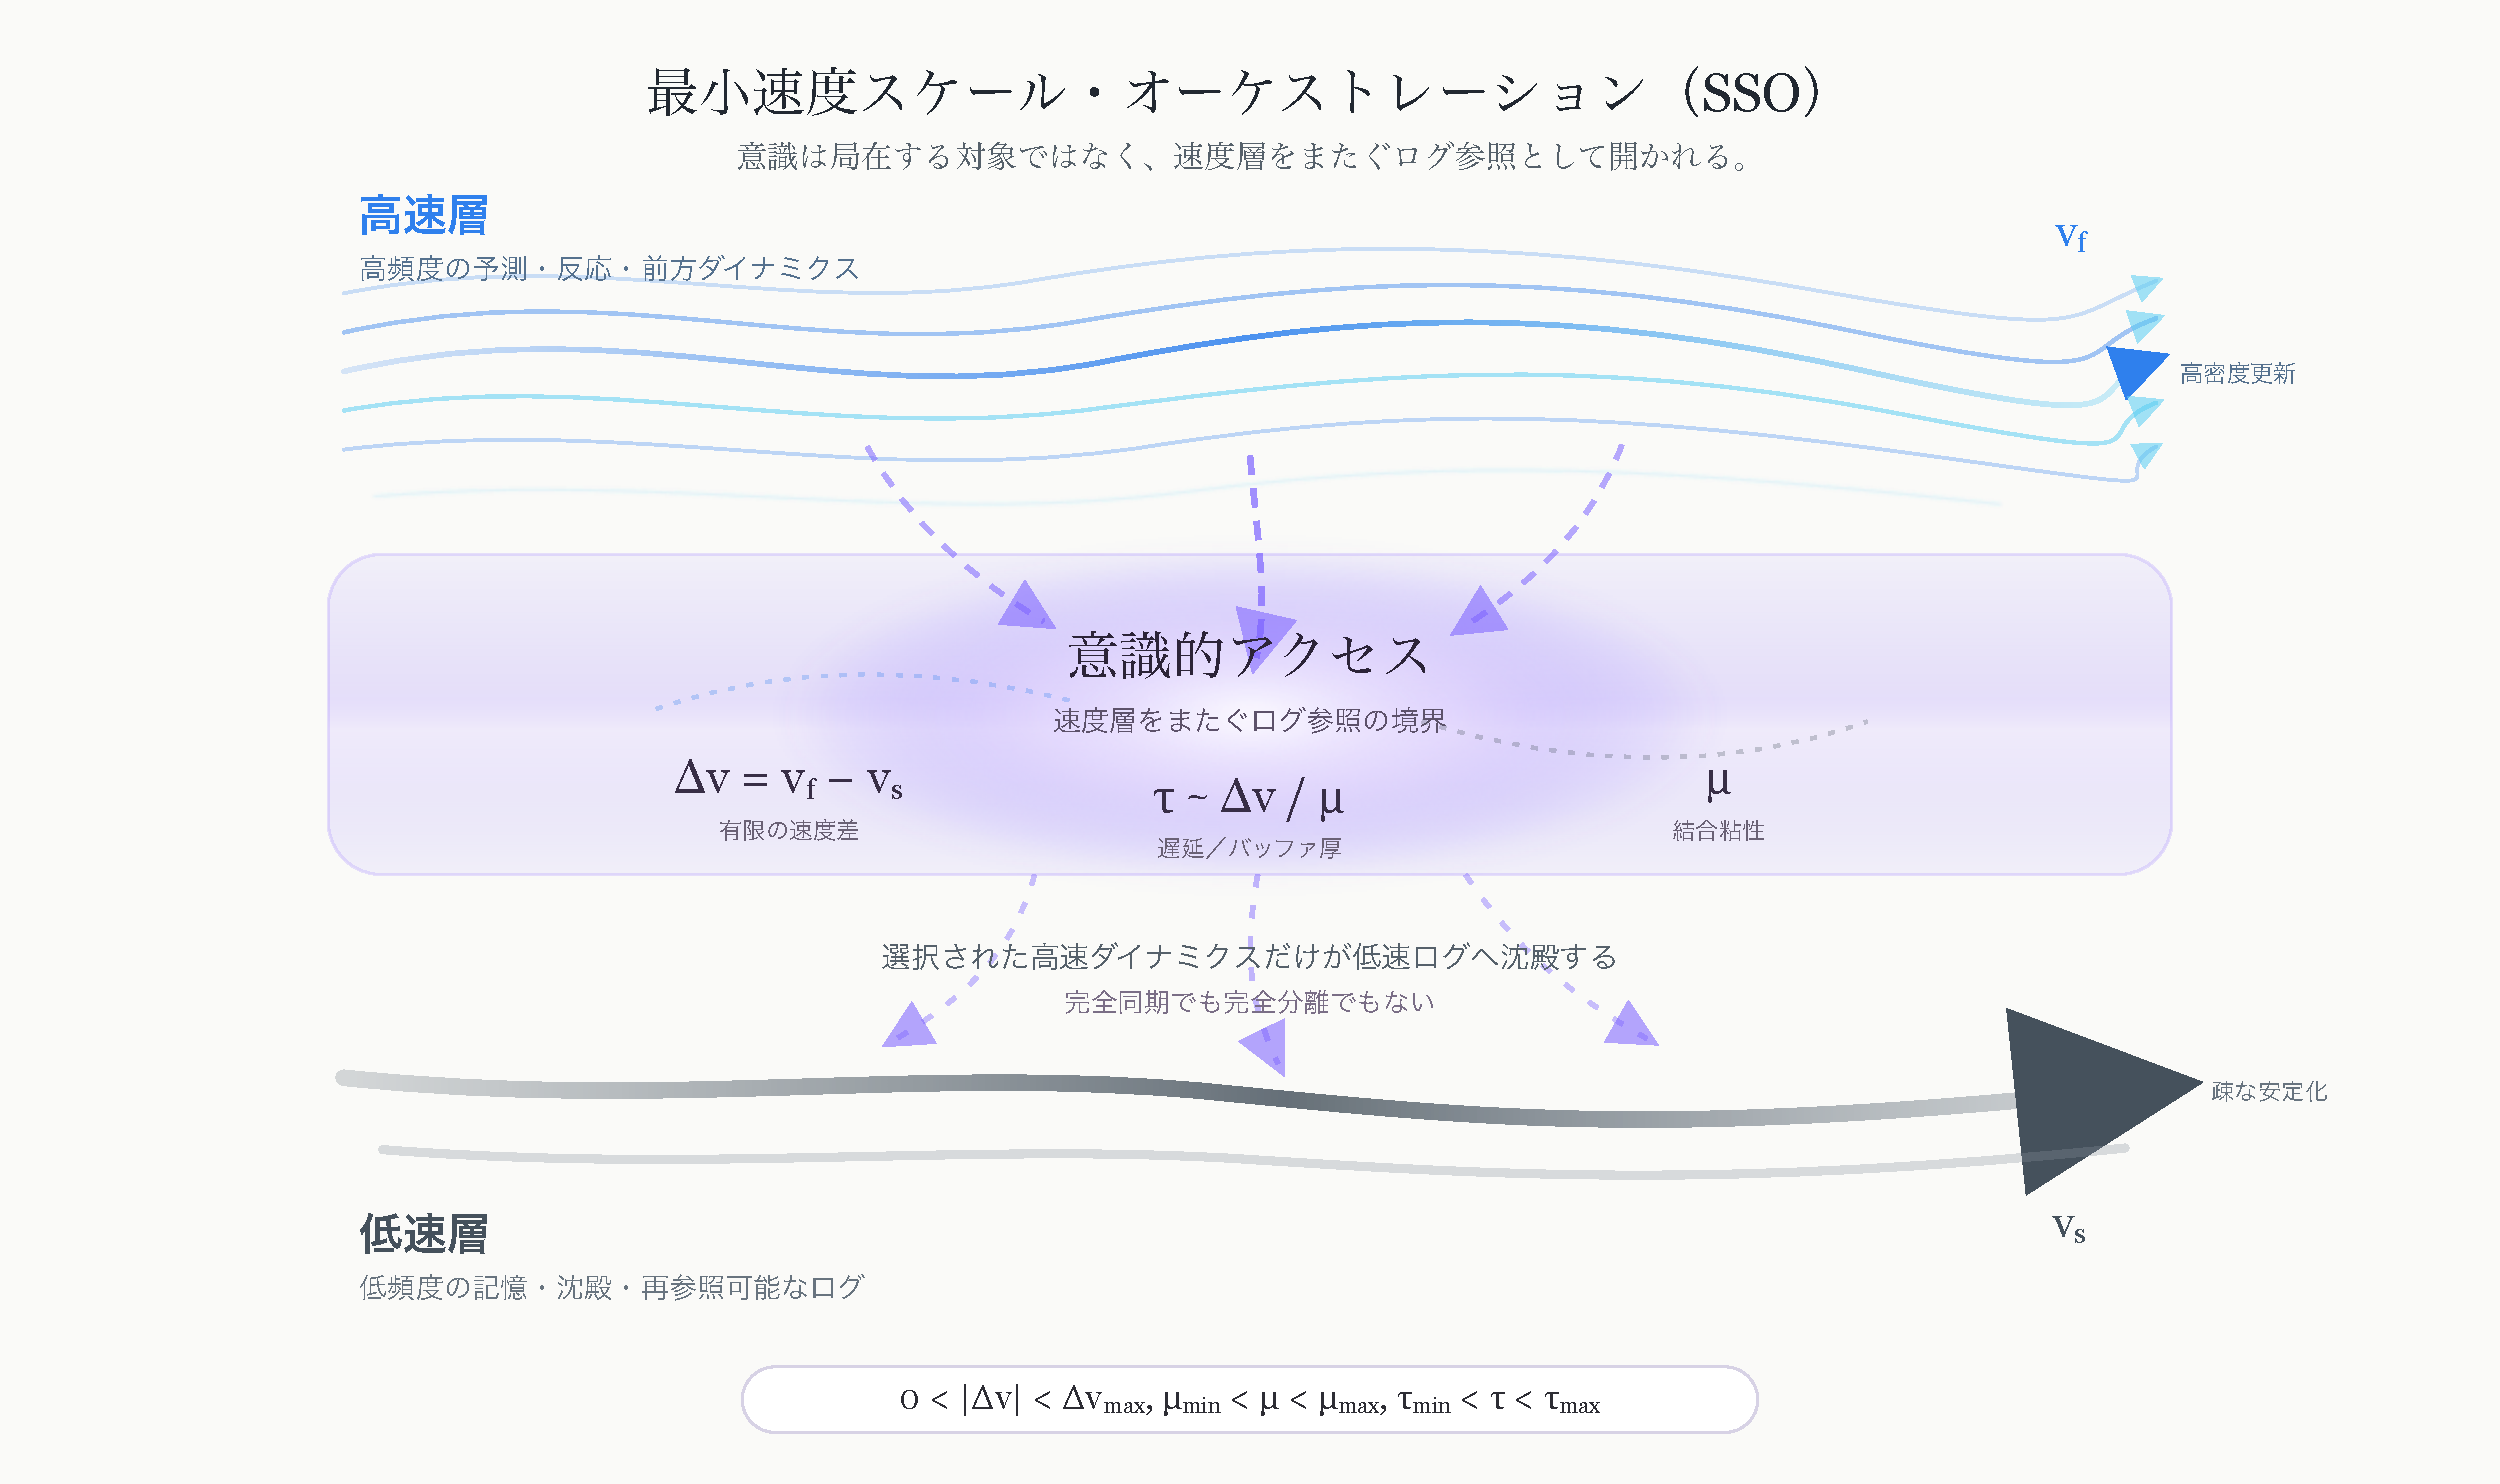
\includegraphics[width=0.92\linewidth]{figures_ja/figure1_sso_density_jp.pdf}
\caption{
Speed-Scale Orchestration（SSO）の最小構造。
意識は高速層または低速層のどちらか一方に局在するのではなく、高速な予測ダイナミクスと低速な沈殿ログが、有限の速度差、遅延、結合粘性のもとで相互参照可能になる境界に開かれる。
}
\label{fig:sso-ja}
\end{figure}

\subsection{Orchestration Without Control}

SSO において、処理層を統括する中央制御者は仮定されない。

高速層が低速層を支配するのでもなく、低速層が高速層を上から制御するのでもない。

両者は、それぞれの時間スケールで独立に走りながら、局所的に干渉する。

ここでいう orchestration とは、指揮者による制御ではない。

それは、異なる速度で走る処理が、互いの差を保ちながら、破綻しない範囲で結合することを意味する。

したがって、SSO は control ではなく coordination である。

より正確には、時間的非同期を完全には解消せず、その非同期を利用可能な構造として保持することである。

\subsection{Gate of Plasticity}

高速層と低速層の相互作用には、可塑性ゲートが必要である。

可塑性ゲートは、何を処理するかを決めるものではない。

それは、高速層の活動が低速層を変更できるかどうか、また低速層の構造が将来の高速過程をどの程度制約するかを調整する。

高速層の活動がすべて低速層へ書き込まれるなら、システムは過剰に硬直する。

逆に、高速層の活動がまったく低速層へ届かなければ、経験は沈殿せず、ログ参照は成立しない。

したがって、可塑性ゲートは開閉のスイッチではない。

それは、速度差、遅延、粘性を伴う時間的な通過条件である。

この通過条件によって、高速な処理の一部だけが低速層へ沈殿し、再参照可能なログとなる。

\subsection{Internal Delay and Buffering}

SSO において、遅延は欠陥ではない。

むしろ、遅延があるからこそ、現在処理と過去ログのあいだに参照可能な厚みが生まれる。

この内部遅延を $\tau$ と表す。

\begin{equation}
\tau \propto \frac{\Delta v}{\mu}
\end{equation}

ここで $\mu$ は、高速層と低速層の結合粘性を表す。

$\tau$ は主観的時間そのものではない。

それは、高速層で生じた処理が低速層へ沈殿し、ログとして参照可能になるまでの内部的な時間バッファである。

$\tau$ が小さすぎれば、処理は即時反応として流れ去り、参照可能なログになりにくい。

$\tau$ が大きすぎれば、現在処理とログ沈殿の対応が崩れ、意識状態は断片化する。

したがって、SSO は単に速い処理と遅い処理の並存ではない。

それは、適切な遅延幅を保持する構造である。

\subsection{SSO as Temporal Non-Closure}

VED の観点から見ると、SSO は時間的非閉包構造である。

高速層と低速層は、閉じようとする。

すなわち、処理は安定化し、沈殿し、ログとして固定されようとする。

しかし、完全に閉じてしまえば、速度差は消え、流れは止まり、意識の境界は失われる。

逆に、閉じなければ、処理は流れ去り、ログとして残らない。

SSO は、この二つの極のあいだにある。

閉じようとするが、閉じ切らない。

分離しようとするが、切れ切らない。

この非閉包的な時間構造の中で、現在処理と過去ログのあいだに参照関係が開かれる。

この意味で、SSO は意識を生成する装置ではない。

SSO は、意識が開かれうる時間的条件である。

\begin{quote}
\textbf{CT との対応（Conceptual Topography §2.4）：} 概念地形論では、低速層が形成する$\Phi$の地形は「意識の閾値以下で動く不可視のGPU」として記述される。思考は地形の上を流れるが、地形そのものは意識から直接参照されない。本稿の低速層／高速層の差が、CTではこの「可視の流れ（$J_I$）と不可視の地形（$\Phi$）の非対称性」として現れる。CTを読んだ後でこの節に戻ると、SSO の時間条件が概念地形の形成条件と同一の構造を持つことが見えてくる。
\end{quote}

\subsection{From SSO to Self-Sustaining Observer}

SSO は、Speed-Scale Orchestration として導入された。

しかし、この構造が安定した時間ループを形成するとき、同じ構造は Self-Sustaining Observer として読まれうる。

ここで observer とは、世界を眺める主体を意味しない。

それは、現在処理、過去ログ、可塑性ゲートが相互に閉じ切らないループを形成し、自己維持的に参照状態を保つ構造を指す。

高速層は未来を先取りする。

低速層は過去を保持する。

可塑性ゲートは、その両者の間で何が沈殿し、何が流れ去るかを調整する。

このループが安定したとき、システムは外部から制御されなくても、自己のログを参照しながら状態を更新できる。

ここに、観測者らしさが現れる。

ただし、それは主体が追加されたからではない。

時間構造が自己維持的になっただけである。

\subsection{Minimal Conditions}

以上をまとめると、SSO が成立するための最小条件は次のように整理できる。

\begin{enumerate}
\item 高速層と低速層が存在すること。
\item 両者のあいだに有限の速度差 $\Delta v$ があること。
\item 速度差が完全同期にも完全分離にも至らないこと。
\item 可塑性ゲートによって、処理の一部が低速層へ沈殿しうること。
\item 内部遅延 $\tau$ が、参照可能な時間的厚みとして保持されること。
\item この構造が中央制御なしに自己維持的ループを形成すること。
\end{enumerate}

この条件が満たされるとき、システムは単なる処理装置ではなく、ログ参照可能な時間構造を持つ。

この構造そのものは、まだ意識ではない。

しかし、この構造がなければ、意識は成立しない。

次節では、この SSO の内部で速度差を破綻なく変換する機構として、トルクコンバータ・アテンションを導入する。


\section{Torque Converter Attention}


通常、注意はフィルタ、重み、選択、抑制として語られる。

どの情報を通すのか。どの対象に焦点を当てるのか。どの表象を強め、どの表象を弱めるのか。

これらの記述は、静的な処理モデルでは有効である。

しかし本稿で扱う意識モデルにおいて、注意の中心問題は選択ではない。

中心にあるのは、異なる速度で走る処理を、同一速度へ潰さずに接続することである。

高速な予測流と低速な記憶流は、そのままでは直接接続できない。

高速層は変化が速く、揮発的であり、現在に先行する。

低速層は変化が遅く、沈殿的であり、過去を保持する。

両者を剛体的に結合すれば、速度差は失われる。

逆に、完全に分離すれば、ログ参照は成立しない。

したがって必要なのは、速度差を消さず、しかし破綻もさせない中間機構である。

本稿では、この機構をトルクコンバータ・アテンションと呼ぶ。

\subsection{Why Filter, Gate, Weight, and Switch Are Insufficient}

既存の注意モデルで頻繁に用いられる語には、それぞれ限界がある。

filter は、通すか通さないかを表すが、速度差そのものを扱えない。

gate は、入口と出口を示すが、内部で生じる滑りや遅延を消してしまう。

weight は、重要度を数値化できるが、処理速度の差を含まない。

switch は、状態の切り替えを表すが、連続的な変換や部分的な結合を表現しにくい。

これらはいずれも、選択や強度を扱う語である。

しかし、本稿で必要なのは、選択の語ではなく、時間変換の語である。

注意とは、何を選ぶか以前に、異なる時間スケールの処理がどのように接続されるかという問題である。

\subsection{Torque Converter as Structural Analogy}

トルクコンバータは、異なる角速度をもつ二つの回転系を剛体的に固定せず、流体的な滑りを許しながら力を伝達する装置である。

ここで重要なのは、速度差が欠陥ではないという点である。

トルクコンバータは、速度差を消してから力を伝えるのではない。

速度差を保持したまま、その差を破綻しない形で伝達可能にする。

この構造は、本稿における高速層と低速層の関係に対応する。

高速層と低速層のあいだには、速度差 $\Delta v$ がある。

\begin{equation}
\Delta v = v_f - v_s
\end{equation}

この速度差がなければ、参照のための境界は開かれない。

しかし速度差が大きすぎれば、参照は断片化する。

したがって必要なのは、差を消す機構ではなく、差を変換する機構である。

これが、トルクコンバータ・アテンションである。

\subsection{Effective Torque}

速度差が変換負荷として現れる量を、有効トルク様量 $\mathcal{T}$ と表す。

\begin{equation}
\mathcal{T}
=
\kappa
\frac{\Delta v}{\mu}
\end{equation}

ここで、$\kappa$ はスケール係数、$\mu$ は結合粘性である。

$\mu$ は、速度スケール間の滑りや結合の粘りを表す。

$\mu$ が小さすぎれば、二つの層は過剰に密着し、速度差が潰れやすくなる。

$\mu$ が大きすぎれば、二つの層は滑りすぎ、参照は不安定化する。

したがって、$\mathcal{T}$ は単なる力の大きさではない。

それは、速度差が結合粘性を介してどれだけ変換負荷として現れるかを表す構造的指標である。

ここで注意すべきなのは、$\mathcal{T}$ を心理的意志や主体性の量として読まないことである。

$\mathcal{T}$ は「どれだけ意識が強いか」を表す量ではない。

それは、異なる速度で走る処理が、ログ参照可能な関係へ変換されるための負荷である。

\cref{fig:tca-ja} は、TCA が速度差を消さずに変換する構造を示している。

\begin{figure}[H]
\centering
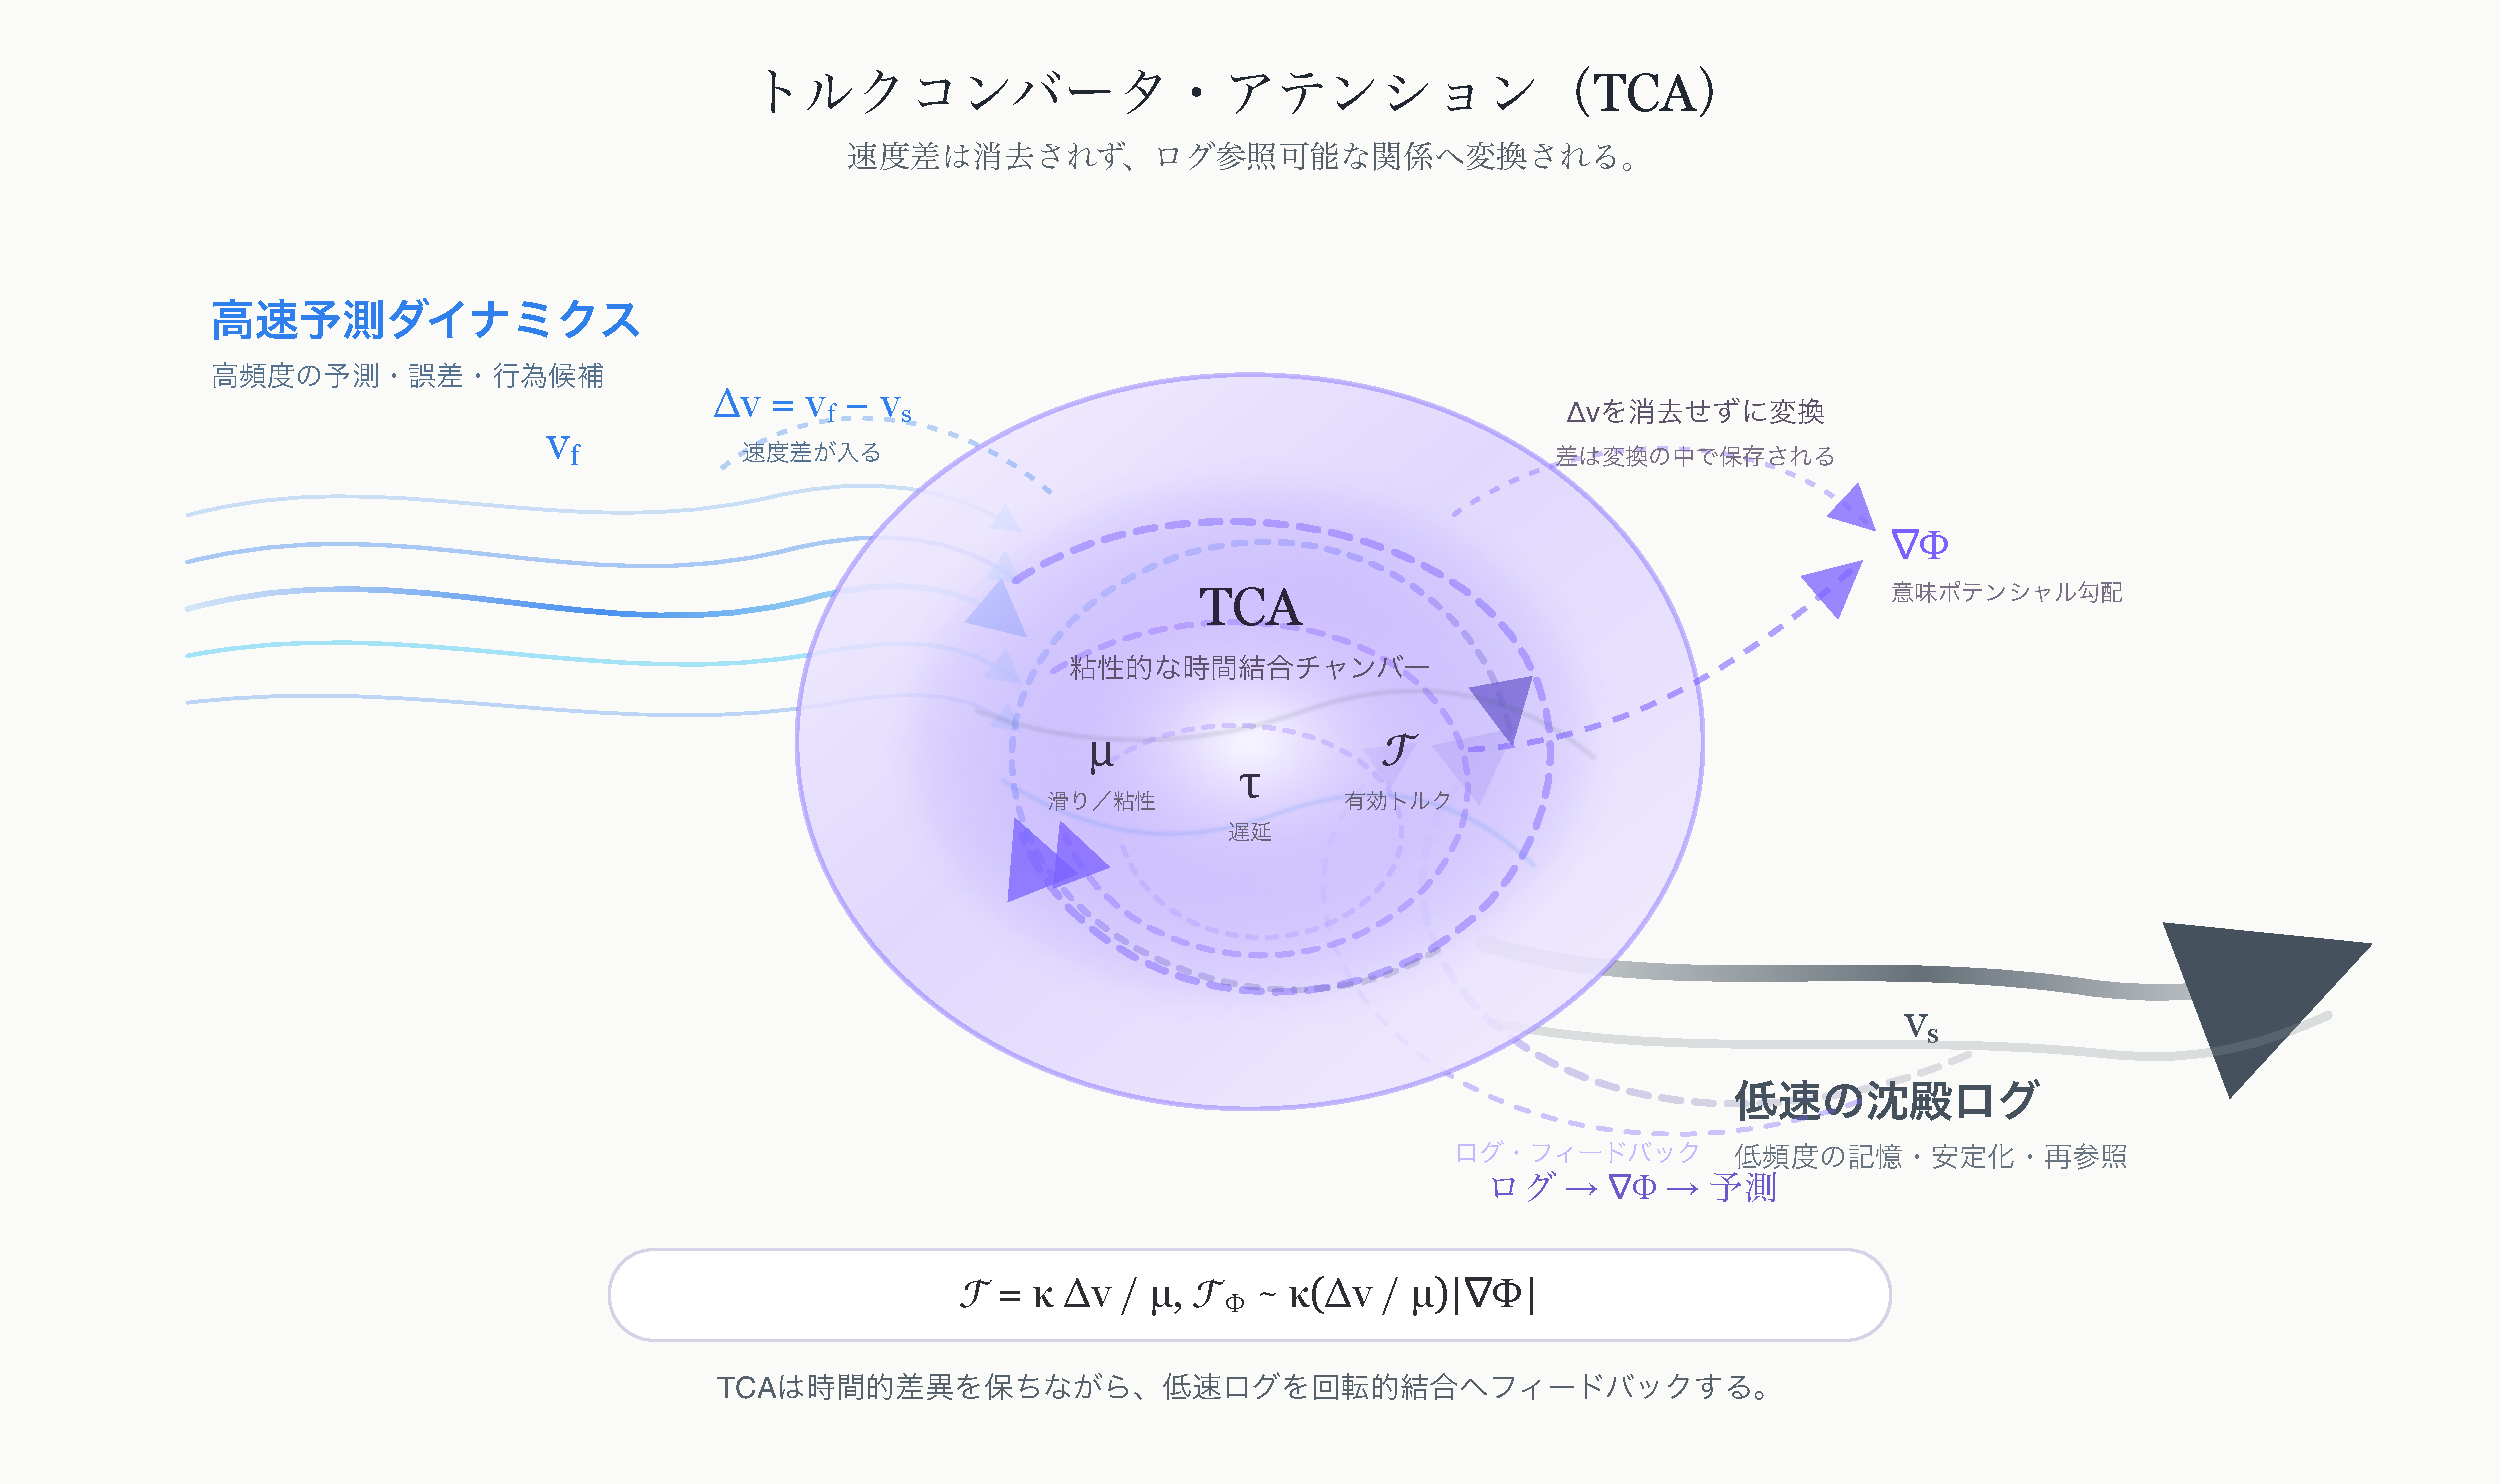
\includegraphics[width=0.92\linewidth]{figures_ja/figure2_tca_jp.pdf}
\caption{
Torque Converter Attention（TCA）。
TCA は時間的差異を保持したまま、それをログ参照可能な関係へ変換する。
高速な予測ダイナミクス、低速な沈殿ログ、結合粘性、遅延、有効トルク様量は、速度差を消去せずに結合される。
}
\label{fig:tca-ja}
\end{figure}

局所的に見れば、あるログまたは概念地形要素 $i$ への注意重み $A_i$ は、そのログの情報質量、または沈殿度 $m_i$ と、局所的な有効トルク様量 $\mathcal{T}_i$ の積として表される。

\begin{equation}
A_i \propto m_i \cdot \mathcal{T}_i
\end{equation}

ここで $\mathcal{T}_i$ は、心理的な意志の量ではなく、高速層と低速層の速度差から生じる局所的な変換負荷である。

\begin{equation}
\mathcal{T}_i \propto \Delta v_i
\end{equation}

したがって、最小近似では次のように書ける。

\begin{equation}
A_i \propto m_i \cdot \Delta v_i
\end{equation}

この式は、注意を単なる選択ではなく、保存されたログの質量と現在の速度差トルクの積として捉えるためのものである。

ここで、SSO の速度差、IFGT の情報ポテンシャル、Conceptual Topography における概念地形要素の沈殿度が接続される。

\subsection{Attention as Temporal Transformation}

この立場から見ると、Attention は選択機構ではなく、時間変換機構である。

Attention は、速い処理を遅い処理へそのままコピーするものではない。

また、遅い処理が速い処理を上から制御するものでもない。

Attention は、高速層で生じた予測、期待、誤差、反応を、低速層が参照可能な時間幅へ変換する。

この変換には遅延 $\tau$ が伴う。

\begin{equation}
\tau \propto \frac{\Delta v}{\mu}
\end{equation}

この遅延は単なる処理遅れではない。

それは、現在処理が過去ログへ沈殿し、再参照可能になるための時間的厚みである。

したがって、Attention は「どこを見るか」ではなく、「どの速度差を、どの時間幅で、どの程度滑らせながら通過させるか」を決める構造である。

この意味で、Attention は心理語ではなく、時間制御語である。

\begin{quote}
\textbf{CT との対応（Conceptual Topography §4.2）：} 概念地形論では、言語トークン $\ell_{i}$ が $\nabla\Phi$ に局所結合し、繰り返し使用によってポテンシャル井戸を深化させる。この結合項
\[
\lambda \sum_i \ell_{i} \cdot \nabla\Phi
\]
は、本稿のTCAが行う「速度差を意味勾配に沿って変換する」操作と対応している。TCAは時間軸上の変換機構であり、CT のトークン結合は空間軸上の変換機構である。両者は同一の変換構造の異なる断面として読める。
\end{quote}

\subsection{From Attention to Ego}

本稿では、このトルクコンバータ・アテンションが、体験上は自我として感じられる位置に対応すると考える。

ただし、ここでいう自我は主体ではない。

自我は判断者でも、司令塔でも、意思決定者でもない。

自我とは、高速層と低速層の速度差が集中し、変換される力学的位置である。

人間はこの変換点を、自分が考えている場所、自分が選んでいる場所、自分が意識している場所として経験しやすい。

しかし、それは自我が行動の原因であることを意味しない。

むしろ、自我とは、行動準備、記憶沈殿、ログ参照が交差する点である。

このため、自我は幻想ではない。

それは明確な機能を持つ。

しかし同時に、自我は主体でもない。

それは、二重可塑性と時間非対称性が成立したときに要請される変換点である。

\subsection{Relation to Log Referencing}

トルクコンバータ・アテンションが重要なのは、それがログ参照を可能にするからである。

高速層で生じた処理は、そのままでは消えていく。

低速層に沈殿したログは、そのままでは現在に接続されない。

両者の間にトルクコンバータ・アテンションが働くことで、現在処理と過去ログの間に参照関係が開かれる。

このとき、高速層の処理は低速層に完全に吸収されるわけではない。

低速層のログも、高速層を完全に支配するわけではない。

両者は、速度差を保持したまま結合する。

この非閉包的な結合が、ログ参照状態としての意識の前提になる。

\subsection{Bridge to IFGT and VED}

ここまでの議論では、トルクコンバータ・アテンションを速度差と結合粘性の問題として定義した。

しかし、意識状態において、どのログが参照されやすいかは速度差だけでは決まらない。

ログ参照は、意味勾配によって方向づけられる。

そのため、次節では情報密度 $I$、情報流 $J_I$、局所的なログ参照流 $J_{\log}$、情報ポテンシャル $\Phi$ を導入し、このトルク様量を IFGT/VED の構造へ写像する。

そこで、有効トルク様量 $\mathcal{T}$ は、意味勾配を含む拡張量 $\mathcal{T}_{\Phi}$ へと拡張される。

\begin{equation}
\mathcal{T}_{\Phi}
\sim
\kappa
\frac{\Delta v}{\mu}
|\nabla \Phi|
\end{equation}

この式は、意識を生成する式ではない。

それは、速度差、結合粘性、意味勾配が同時に成立したとき、ログ参照がどの方向へ開かれやすいかを示す構造的指標である。

したがって、トルクコンバータ・アテンションは、本稿において単なる比喩ではない。

それは、速度差を非閉包のまま保持する VED 的機構であり、意味勾配に沿ってログ参照を方向づける IFGT 的機構でもある。


\section{Formal Mapping to IFGT and VED}


本節では、本稿で扱う意識モデルを IFGT および VED のフレームワークへ写像する。

ここで行うのは、意識を物理場へ還元することではない。また、脳内現象をそのまま宇宙論的方程式へ対応させることでもない。

本節の目的は、意識を、情報流・意味ポテンシャル・非閉包ダイナミクスの局所的かつ射影的な実装として読むための最小対応を固定することである。

\subsection{投影的使用と projection 操作}
\label{sec:projected-uses}

IFGT との対応を提示する前に、本節は本稿全体で使われている語彙の方法論的地位を固定し、IFGT の第四の構造的基礎概念としての projection の構造論的定義を明示する。

この議論を IFGT 対応の前に置く理由は単純である。$I$、$J_I$、$\Phi$、および局所的な log-referencing 流 $J_{\log}$ が導入されるとき、つねに二つの異なる問いが同時に存在する。これらの変数が一般 IFGT 場において何を指すか、そして本稿がこれらを生物-認知観測窓のなかでどのように用いているか、である。この二つの読みを混同することは、場の理論的語彙に基づく意識モデルにおいて繰り返し誤解を生んできた。本稿の立場をあらかじめここで固定する。

\subsubsection{立場：投影的使用}
\label{sec:projected-uses-stance}

本稿では、IFGT 変数は一般情報場との直接的同定としてではなく、特定の観測窓のなかで投影された変数として用いられる。

具体的には、次のように読む。

\begin{itemize}
\item $I$、$J_I$、$\Phi$ は本稿において、生物-認知窓のなかでの有効座標として現れる。IFGT 場そのものとしてではない。
\item 局所的 log-referencing 流 $J_{\log}$ は窓-局所的な流量変数として扱われる。大域的 IFGT 流としてではない。
\item これらの変数を含む方程式は、この窓の記述として読まれるべきであって、普遍的情報場についての存在論的主張として読まれるべきではない。
\end{itemize}

この立場を投影的使用（projected uses）と呼ぶ。これは並行論文である知性編 \cite{Intelligence} で採られているのと同じ方法論的立場であり、両論文はこの立場を共通の認識論的基盤として共有する。

二つの帰結が従う。

第一に、§§7--9 の方程式は意識の普遍的場の方程式であると主張するものではない。それらは本稿が意識を記述する生物-認知窓のなかで成立する構造的関係である。

第二に、本稿が VED、Bio-IFGT、Conceptual Topography (CT)、または知性編との対応を述べるとき、その対応は同一の差分発展構造の、異なる投影窓どうしの関係として読まれるべきであって、ある記述が別の記述に還元される関係ではない。いずれの論文も他を基礎づけはしない。各論文は窓-局所的な記述である。

\subsubsection{IFGT 第四基礎概念としての projection}
\label{sec:projection-definition}

情報密度 $I$、情報流 $J_I$、情報場ポテンシャル $\Phi$ に加えて、本稿は第四の構造的基礎概念として projection（質量割当）を用いる。

\paragraph{定義}
projection とは、特定の状態または表象が、動態のなかで不均衡な影響力を獲得する操作である。

\begin{itemize}
\item projection は注意・選択・優先化の構造的記述である。
\item projection は意図的選択を要求しない。物理的偏向、生物学的優先化、人工的重み付けのすべてを含む。
\item projection は $\Phi$ と $J_I$ を結ぶ機構である。大域的バイアスが具体的な状態に局所化する操作である。
\end{itemize}

本稿の言葉で言えば、slow layer がどの log を強化するか、fast layer のどの活動が plasticity gate を通過するか、$\nabla\Phi$ が $J_{\log}$ にどの方向を課すか。これらはすべて、生物-認知窓における projection の具体例である。§5 および §7 で導入された有効トルク様量 $\mathcal{T}_{\Phi} \sim \kappa (\Delta v / \mu)\,|\nabla\Phi|$ は、意識窓の各瞬間において projection がどれほど強く作動しているかの構造的指標である。

projection は本稿のなかで、明示的に名指されなくても常に荷重的役割を果たしてきた。plasticity gate、meaning gradient によるバイアス、§13 における qualia 残余の選択、§10 の split-brain における referencing pathway の非対称性。これらはすべて、構造的には異なる局所条件のもとでの projection 操作である。

\subsubsection{心理学的 projection との関係}
\label{sec:projection-disclaimer}

projection という用語は心理学、特に精神分析的伝統においても用いられ、そこでは主体が自身の内的状態を他者または外部対象に投影する機制を意味する。用語の重なりは現実に存在するが、構造論的地位は同一ではない。

心理学的 projection は主体・無意識・内部状態の存在を前提する。本稿で用いる IFGT における projection は、これらをいずれも公理レベルでは前提しない。両概念は「重みの不均衡配分」という構造的特徴を共有しており、心理学的 projection は IFGT projection の、特定層における運用論的記述、すなわち主体性を持つ複雑系の表層における具体的現れとして読みうる。

両概念のどちらが他方を還元するわけではない。両者は同じ構造を異なる粒度で記述している関係にある。本稿は構造論的水準のみを扱い、心理学的概念との詳細な対応は射程外とする。本稿の他の箇所で「projection」と書かれている場合は、構造論的意味のみが意図されている。

\subsubsection{本節が主張しないこと}
\label{sec:projected-uses-non-claims}

明確化のため、二つの非主張を明示しておく。

\begin{itemize}
\item 本節は、意識窓が一般 IFGT 場の特定断面と同一であるとは主張しない。両者の関係は、上で固定された意味での projection 関係である。
\item 本節は、生物-認知窓、知性層窓、概念地形窓が相互に還元可能であるとは主張しない。これらは同一の差分発展構造の異なる投影窓として記述されるのであり、窓間動力学の問題は別所で扱われる（\cite{Intelligence}, §9.4）。
\end{itemize}

これらの明確化のもとで、§6 の残りは本節で固定された投影的使用の意味で意識モデルを IFGT および VED に対応づけていく。読者は以下、$I$、$J_I$、$J_{\log}$、$\Phi$、および projection を、窓-局所的な構造的基礎概念として読むべきであって、完全な IFGT 場としては読むべきではない。

\subsection{IFGT Mapping: Information, Flow, Potential}

IFGT の基本変数は、情報密度 $I$、情報流 $J_I$、情報場ポテンシャル $\Phi$、および projection（§\ref{sec:projection-definition}）である。

§\ref{sec:projected-uses-stance} で固定された投影的使用の意味で、本稿ではこれらを生物-認知窓における有効座標として用いる。すなわち、$I$、$J_I$、$\Phi$ は一般 IFGT 場との直接的同定ではなく、log 沈殿・log referencing・意味勾配バイアスを記述するための窓-局所的有効座標である。projection はこれら諸変数を結ぶ操作として、§\ref{sec:projected-uses} の構造論的定義のもとで以下のマッピング全体を貫いて作動している。

本稿では、意識モデルにおける各要素を次のように対応させる。

\begin{itemize}
\item $I$：低速層に沈殿したログ密度。
\item $J_{\log}$：高速層から低速層へ向かう処理流、またはログ参照の流れ。
\item $\Phi$：ログ配置が作る情報ポテンシャル、すなわち意味場。
\item $\nabla \Phi$：どのログが参照されやすいかを方向づける意味勾配。
\item $\partial \Phi / \partial t$：意味場のライブな変化。
\end{itemize}

ここで $I$ は、単なる記憶量ではない。

それは、再参照可能な形で沈殿したログの密度である。

また、$J_{\log}$ は単なる情報伝達ではない。

それは、現在の処理がどのログへ向かい、どのログを更新し、どの意味井戸へ流れ込むかを表す動的な流れである。

$\Phi$ は、ログに「意味」が内在していることを表すものではない。

意味はログの中に保存されているのではなく、ログ同士の配置が作るポテンシャルとして張られる。

したがって、意識状態におけるログ参照は、低速層に保存された内容を単に取り出す過程ではない。

それは、現在の高速処理が、既存の情報ポテンシャルの勾配に沿って低速層へ接続される過程である。

\subsection{IFGT Core Relations}

IFGT の最小関係は、次の形で与えられる。

\begin{equation}
\frac{\partial I}{\partial t} + \nabla \cdot J_I = \sigma
\end{equation}

\begin{equation}
J_I = -D \nabla I + \mu_I F
\end{equation}

\begin{equation}
F = -\nabla \Phi
\end{equation}

\begin{equation}
\Phi = K * I
\end{equation}

ここで、$\sigma$ は情報密度の生成・散逸項、$D$ は拡散係数、$\mu_I$ は情報流の移動係数、$F$ は情報ポテンシャルから生じる有効力、$K$ は情報密度からポテンシャルを与える核である。

本稿では、これらを意識の完成した方程式として用いるのではない。

これらは、ログ参照がどのような射影場の中で方向づけられるかを記述するための構造的テンプレートである。

すなわち、意識は $I$ そのものではない。

意識は $J_I$ そのものでも、$J_{\log}$ そのものでもない。

意識は $\Phi$ そのものでもない。

意識は、情報密度、情報流、情報ポテンシャルが、時間スケール差をもつ処理系の中で相互に接続されるときに開かれる状態である。

\subsection{VED Mapping: Non-Closure as Condition}

VED の基底にあるのは、完全閉包を通常の到達可能状態として扱わない動的構造である。

差があり、勾配が立ち、流れが生じ、構造は閉包へ向かう。しかし完全閉包は、通常の生成状態としては実現されない。

この非閉包性が、運動の持続条件である。

意識モデルにおいても、同じ構造が現れる。

高速層と低速層が完全に同期すれば、速度差 $\Delta v$ は消える。

\begin{equation}
\Delta v \rightarrow 0
\end{equation}

このとき、処理は滑らかに自動化されるが、ログ参照のための境界は消える。

逆に、高速層と低速層が完全に分離すれば、流れ $J_{\log}$ は低速層へ到達しない。

このとき、処理は起きても、参照可能なログとして沈殿しない。

したがって、意識状態は完全同期でも完全分離でもない。

それは、差が残り、流れが保たれ、しかし破綻しない非閉包レジームである。

この最小条件は次のように書ける。

\begin{equation}
\Delta v \neq 0
\end{equation}

ただし、これは速度差が大きければよいという意味ではない。

必要なのは、有限の速度差が、結合粘性 $\mu$ によって破綻なく保持されることである。

この意味で、SSO は脳内における時間的非閉包構造である。

\subsection{VED Closure Degree and the SSO Window}

この節は、VED側の形式化を必要とする読者のための補助的写像である。
直観的理解には、$\Delta v$ を時間スケール差として読むだけで十分である。

VED では、任意の二節点 $i, j$ のあいだの閉包度を次式で定義する。

\begin{equation}
C_{ij} = 1 - \exp\!\left(-\lambda \rho_i H_{ij}\right)
\end{equation}

ここで、$\rho_i$ は節点 $i$ における差の密度、$H_{ij}$ は節点間の接続強度、$\lambda$ はスケール係数である。

$C_{ij} \to 1$ は完全閉包境界であり、差が消え、流れが停止し、生成された記述が依存していた区別を失う点に対応する。

$C_{ij} \to 0$ は完全非閉包であり、節点間の接続が成立していない状態に対応する。

意識モデルへの写像は、次のように行われる。

高速層の有効閉包度を $C_f$、低速層の有効閉包度を $C_s$ とする。

高速層は予測的・揮発的であるため、閉包が進みにくい。すなわち $C_f$ は比較的低い値を維持する。

低速層は沈殿的・安定的であるため、閉包が進みやすい。すなわち $C_s$ は $C_f$ より高い値を取りやすい。

この非対称性から、閉包度差を次のように定義する。

\begin{equation}
\Delta C = C_s - C_f
\end{equation}

この $\Delta C$ は、本稿で用いてきた速度差 $\Delta v$ に対応する構造的量である。

\begin{equation}
\Delta v \;\leftrightarrow\; \Delta C
\end{equation}

すなわち、速度差は「処理の時間スケール差」として導入されたが、VED の言語では「二層のあいだの閉包度差」として読み替えられる。

意識状態が成立するための窓条件は、閉包度差の言葉で次のように書ける。

\begin{equation}
0 < \Delta C < \Delta C_{\max}
\end{equation}

$\Delta C = 0$ は完全同期に対応する。高速層と低速層が同一の閉包度に達し、参照のための境界が消える。

$\Delta C \to \Delta C_{\max}$ は参照断絶に対応する。閉包度の乖離が大きすぎ、高速層の処理が低速層へ届かなくなる。

したがって、意識の consciousness window は、VED の言語では $\Delta C$ が有限の非ゼロ値を保持する閉包度差レジームとして表現される。

\cref{fig:sso-ved-mapping-ja} は、SSO と VED の記述の構造的対応を示している。

\begin{figure}[H]
\centering
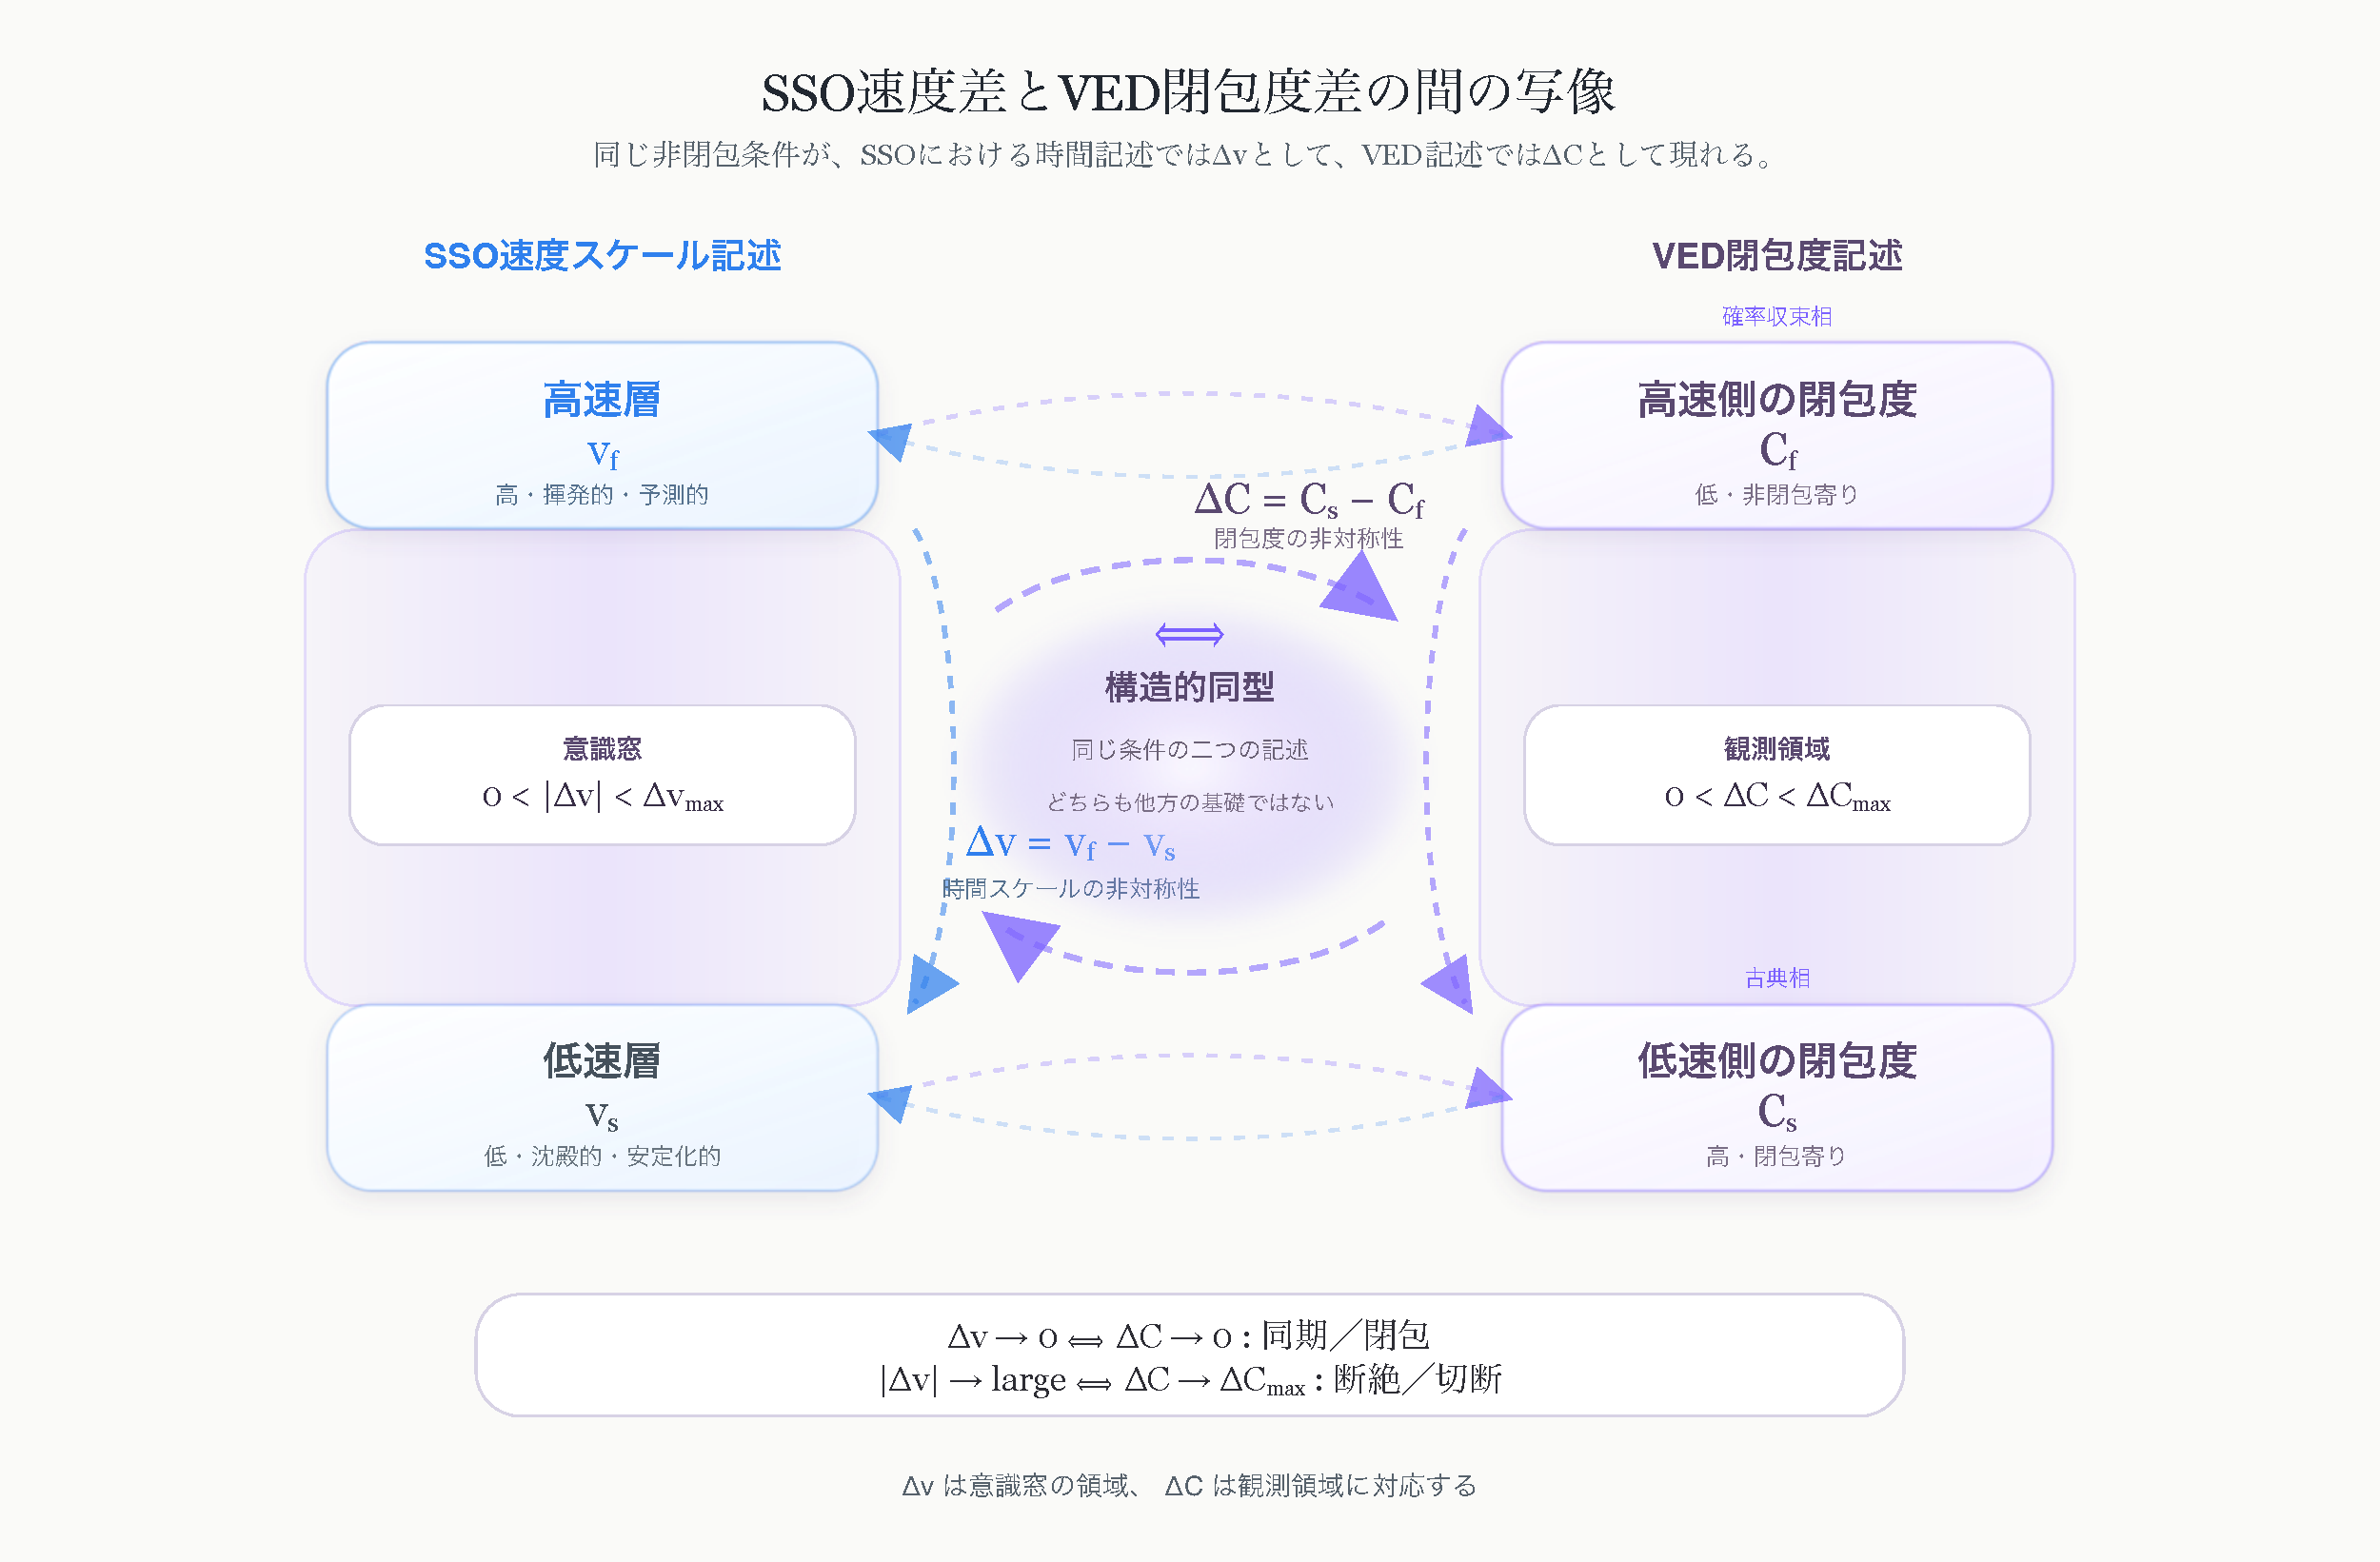
\includegraphics[width=0.94\linewidth]{figures_ja/figure6_observation_regime_jp.pdf}
\caption{
SSO の非対称性と VED の閉包度非対称性の対応。
SSO における速度差 $\Delta v$ と、VED における閉包度差 $\Delta C = C_s - C_f$ は、同じ非閉包条件を異なる座標で記述している。
SSO 側の consciousness window は、VED 側の observation regime に構造的に対応するが、どちらか一方が他方を基礎づけるわけではない。
}
\label{fig:sso-ved-mapping-ja}
\end{figure}

また、旧来の VED における非閉包持続条件

\begin{equation}
\frac{\partial C}{\partial t} + \nabla \cdot J_C = a\Delta\!\left(1 - C/C_*\right) - \Gamma C - \frac{\kappa_B}{C_{\max} - C}
\end{equation}

は、意識モデルにおいて現象論的・粗視化的な近似として次のように読まれる。

第一項 $a\Delta(1 - C/C_*)$ は、差の駆動による閉包への傾向を表す。高速層が低速層を引き寄せようとする力に対応する。

第二項 $-\Gamma C$ は、閉包が進みすぎることへの散逸を表す。完全同期を妨げる項であり、速度差が消滅しないための条件を与える。

第三項 $-\kappa_B/(C_{\max} - C)$ は、閉包が飽和限界に近づくにつれて増大する現象論的な有効障壁を表す。Vol.4 改訂後の解釈では、これは基本的な外部禁止壁ではない。完全閉包が生成された記述の内部で通常状態として実現されないという事実を、射影的な抵抗項として要約したものである。

この三項構造により、SSO は完全閉包にも完全分離にも至らない中間レジームを自己維持的に保つ。

これが、意識状態の非閉包持続条件のVED的根拠である。

\subsection{SSO as Local Non-Closure}

SSO（Speed-Scale Orchestration）は、複数の時間スケールをもつ処理が、中央制御なしに調整される構造である。

VED の観点から見れば、SSO は閉じきらない時間構造の局所モデルである。

高速層は予測し、低速層は沈殿する。

高速層は先に進み、低速層は遅れて固定する。

この差は消されない。

むしろ、この差が残るからこそ、現在処理と過去ログのあいだに参照関係が生まれる。

SSO が成立する条件は、次の三つである。

\begin{enumerate}
\item 高速層と低速層の速度差が存在すること。
\item 両層が完全には分離していないこと。
\item 低速層への沈殿が完全には閉じきっていないこと。
\end{enumerate}

この三条件が満たされるとき、処理は現在に流れ去るだけでなく、過去ログとの関係を開く。

ここに、ログ参照としての意識状態が成立する。

\subsection{Torque Converter Attention as IFGT/VED Coupler}

トルクコンバータ・アテンションは、IFGT と VED の接続点である。

VED 的には、それは速度差 $\Delta v$ を消さずに伝達する非閉包機構である。

IFGT 的には、それは情報ポテンシャル $\Phi$ の勾配に沿って、どのログが参照されやすいかを調整する機構である。

このため、有効トルク様量 $\mathcal{T}$ は、まず速度差と結合粘性によって表される。

\begin{equation}
\mathcal{T} =
\kappa
\frac{\Delta v}{\mu}
\end{equation}

しかし、意識状態において参照されるログは、速度差だけで決まらない。

ログ参照は意味勾配によって方向づけられる。

したがって、意識モデルにおける有効量は、情報ポテンシャルの勾配を含んだ形に拡張される。

\begin{equation}
\mathcal{T}_{\Phi}
\sim
\kappa
\frac{\Delta v}{\mu}
|\nabla \Phi|
\end{equation}

ここで $\mathcal{T}_{\Phi}$ は、時間スケール差と意味勾配が結合した有効トルク様量である。

これは意識を生成する量ではない。

それは、ログ参照がどの程度強く、どの方向へ開かれやすいかを示す構造的指標である。

\subsection{Consciousness as IFGT/VED Interface}

以上を踏まえると、本稿における意識は、IFGT と VED の交差面における局所的な射影レジームとして位置づけられる。

IFGT は、ログ、意味場、情報流の配置を与える。

VED は、その配置が完全閉包を通常状態として実現せず、差と流れを保ち続ける条件を与える。

意識は、この二つの記述が重なるところでモデル化される。

すなわち、意識とは、射影された情報ポテンシャルに方向づけられたログ参照が、完全同期にも完全分離にも至らない時間的非閉包レジームの中で開かれている状態である。

これを最小形で書けば、次のようになる。

\begin{equation}
\text{Consciousness}
\sim
\text{Log Referencing}
\left(
I,
J_{\log},
\Phi,
\Delta v,
\mu,
\tau,
\mathcal{T}_{\Phi}
\right)
\end{equation}

この式は、意識を計算する式ではない。

それは、意識について語るときに必要な構造変数を示す座標である。

意識は、$I$ だけに還元されない。

$J_I$ だけにも、$J_{\log}$ だけにも、$\Phi$ だけにも、$\Delta v$ だけにも還元されない。

意識は、それらが時間的非閉包状態の中で結合したときに開かれる。

\paragraph{差分発展構造の投影としての位置づけ}
本節で固定された IFGT/VED 界面における意識の位置は、より広い構造の中に置かれている。VED は物理層を、Bio-IFGT は生命層を、本稿は意識層を、知性編 \cite{Intelligence} は知性層をそれぞれ記述する。これら四層は同一の差分発展構造を異なる粒度で繰り返しており、各論文はそのうちのひとつの投影窓を記述している。

§\ref{sec:projected-uses-stance} で固定された投影的使用の立場は、この複数窓間の関係を「相互還元」ではなく「同一構造の異なる投影」として読むことを要請する。本稿の意識窓と他層との対応の詳細は §20 で整理される。

\subsection{Why This Mapping Is Minimal}

本節の写像は、意図的に最小限にとどめられている。

理由は二つある。

第一に、意識を過剰に形式化すると、意識を閉じた対象として扱ってしまう危険がある。

しかし本稿の立場では、意識は完全閉包された対象ではなく、非閉包的なログ参照状態である。

第二に、IFGT/VED の役割は、意識を説明しきることではなく、意識についての問いを正しい位置へ置くことである。

したがって、本節では意識の統一方程式を与えない。

与えるのは、意識がどの変数のあいだに開かれるかという、最小対応である。

この最小写像によって、本稿は次節で中核方程式を整理できるようになる。

すなわち、速度差、結合粘性、内部遅延、有効トルク様量、意味勾配、非閉包条件を、同一の構造の中で扱うことが可能になる。


\section{Core Equations}


本稿で用いる方程式は、意識そのものを閉じた形で定義するためのものではない。

意識は保存量ではなく、加算的な量でもなく、単一の変数として測定される対象でもない。したがって、ここで提示する式は「意識の方程式」ではない。

ここで固定するのは、意識が成立しうる有効領域である。

すなわち、高速な予測過程、低速な記憶沈殿過程、両者の速度差、結合粘性、情報ポテンシャルの勾配が、どのような関係にあるときログ参照状態が開かれるのかを記述する。

\subsection{Speed Differential}

まず、高速層と低速層の速度差を次のように置く。

\begin{equation}
\Delta v = v_f - v_s
\end{equation}

ここで、$v_f$ は高速な予測的・反応的ダイナミクス、$v_s$ は低速な沈殿的・安定化的ダイナミクスを表す。

重要なのは、$v_f$ または $v_s$ が単独で意識を定義するのではないという点である。

意識に関わるのは、それらの絶対速度ではなく、両者のあいだに維持される差である。

VED 的に言えば、完全同期は閉包であり、差の消失である。差が完全に消えるなら、境界も流れも失われる。

したがって、意識状態が維持されるための最小条件は次のように表せる。

\begin{equation}
\Delta v \neq 0
\end{equation}

これは、意識が常に強い非同期を必要とするという意味ではない。

むしろ、完全同期に潰れず、かつ完全分離にも至らない有限の速度差が必要である、という意味である。

ただし、$\Delta v$ は意識そのものではない。

$\Delta v$ は、高速層と低速層のあいだに残るズレであり、ログ参照の境界を開くための条件である。

この関係を最小限に書けば、意識的アクセス、または意識の開き $C(t)$ は、速度差、低速層におけるログ密度、参照が持続する時間幅の関数として表される。

\begin{equation}
C(t) \propto \mathcal{F}(\Delta v, \rho_s, \tau)
\end{equation}

ここで、$\rho_s$ は低速層に沈殿したログ密度であり、ログがどれだけ重みを持って再参照可能になっているかを表す。

$\tau$ は、ログ参照が持続する時間スケールである。

したがって、意識は速度差そのものではなく、速度差 $\Delta v$、沈殿したログの重さ $\rho_s$、参照時間 $\tau$ が同時に成立する非閉包状態として開かれる。

\subsection{Coupling Viscosity}

速度差が存在するだけでは、意識状態は成立しない。

高速層と低速層が完全に分離していれば、処理は走っていてもログ参照は起きない。逆に、結合が強すぎて両者が同一速度に潰れれば、参照のための境界が消える。

この結合状態を、結合粘性 $\mu$ によって表す。

\begin{equation}
\mu > 0
\end{equation}

$\mu$ は、高速層と低速層のあいだの滑りやすさ、または結合の粘りを表す。

$\mu$ が小さすぎれば、両層は過剰に結合し、速度差が潰れやすくなる。

$\mu$ が大きすぎれば、両層は滑りすぎ、ログ参照は断片化しやすくなる。

したがって、意識に必要なのは、単なる結合ではなく、速度差を保持したまま相互作用できる粘性領域である。

\subsection{Internal Delay}

速度差と結合粘性の関係は、内部遅延または時間バッファ $\tau$ として現れる。

\begin{equation}
\tau \propto \frac{\Delta v}{\mu}
\end{equation}

$\tau$ は、処理が低速層へ沈殿し、参照可能なログとして整列するまでの内部遅延を表す。

この遅延は欠陥ではない。

むしろ、遅延があるからこそ、即時的な処理はそのまま消えず、ログとして低速層へ到達する余地を得る。

$\tau$ が小さすぎれば、処理は即時反応に近づき、参照可能な厚みを持たない。

$\tau$ が大きすぎれば、現在処理とログ沈殿の対応が崩れ、意識状態は断片化する。

したがって、意識状態は次のような中間領域に存在する。

\begin{equation}
\tau_{\min} < \tau < \tau_{\max}
\end{equation}

この範囲を、本稿では意識安定窓と呼ぶ。

\subsection{Effective Torque}

次に、速度差が単なる遅延ではなく、参照を開くための変換負荷として現れる量を定義する。

本稿ではこれを有効トルク様量 $\mathcal{T}$ と呼ぶ。

\begin{equation}
\mathcal{T} = \kappa \frac{\Delta v}{\mu}
\end{equation}

ここで $\kappa$ はスケール係数である。

$\mathcal{T}$ は心理的な意志や主体性を表すものではない。

それは、高速層と低速層の速度差が、破綻せずに変換されるために必要となる構造的負荷を表す。

トルクコンバータ・アテンションとは、この $\mathcal{T}$ を処理可能な形に変換する機構である。

重要なのは、$\mathcal{T}$ が差を消すのではなく、差を保持したまま伝達するための量だという点である。

\subsection{IFGT Coupling}

ここまでの式は、速度差と結合粘性だけを扱っていた。

しかし、意識状態において参照されるログは、任意に選ばれるわけではない。

どのログが参照されやすいか、どの処理が低速層へ沈殿しやすいかは、情報ポテンシャル $\Phi$ の勾配によって偏る。

IFGT の一般変数を、情報密度 $I$、情報流 $J_I$、情報ポテンシャル $\Phi$ とする。

本稿では、これらを生物的・認知的観測窓に射影された変数として用いる。
したがって $I$、$J_I$、$\Phi$ は、意識と一般 IFGT 場を直同一視するためのものではない。意識編の局所的な流れは $J_{\log}$ と書き、ログ参照流を記述する有効座標として用いる。

基本関係は次のように置かれる。

\begin{equation}
\frac{\partial I}{\partial t} + \nabla \cdot J_I = \sigma
\end{equation}

\begin{equation}
J_I = -D \nabla I + \mu_I F
\end{equation}

\begin{equation}
F = -\nabla \Phi
\end{equation}

\begin{equation}
\Phi = K * I
\end{equation}

ここで、$\sigma$ は情報密度の生成・散逸項、$D$ は拡散係数、$\mu_I$ は情報流の移動係数、$K$ は情報密度からポテンシャルを与える核である。

本稿の文脈では、$\Phi$ は意味や情報のポテンシャルとして働く。

したがって、ログ参照は単なる速度差の関数ではなく、意味勾配によって方向づけられる。

この効果を含めると、有効トルク様量は次のように拡張される。

\begin{equation}
\mathcal{T}_{\Phi}
\sim
\kappa
\frac{\Delta v}{\mu}
\left|\nabla \Phi\right|
\end{equation}

$\mathcal{T}_{\Phi}$ は、時間スケール差と意味勾配が結合した有効量である。

速度差が大きくても、意味勾配が弱ければ、ログ参照は安定した方向を持たない。

逆に、意味勾配が強くても、速度差が消えていれば、参照のための境界は開かれない。

意識状態に関わるのは、この両者の結合である。

\subsection{Consciousness Window}

以上をまとめると、意識状態は次の条件を満たす領域として表される。

\begin{equation}
0 < |\Delta v| < \Delta v_{\max}
\end{equation}

\begin{equation}
\mu_{\min} < \mu < \mu_{\max}
\end{equation}

\begin{equation}
\tau_{\min} < \tau < \tau_{\max}
\end{equation}

\begin{equation}
\mathcal{T}_{\min}
<
\mathcal{T}_{\Phi}
<
\mathcal{T}_{\max}
\end{equation}

これらは、意識を数値的に測定するための完成した式ではない。

むしろ、意識が成立しうる領域を制約する条件である。

速度差がゼロになれば、境界は同期に潰れる。

速度差が大きすぎれば、参照は破断する。

結合粘性が低すぎれば、層は癒着する。

結合粘性が高すぎれば、層は滑りすぎる。

意味勾配が弱すぎれば、ログ参照は方向を失う。

意味勾配が強すぎれば、参照は特定の井戸へ過剰に固定される。

したがって、意識は一点ではなく、窓である。

この窓を、本稿では consciousness window と呼ぶ。

\cref{fig:consciousness-window-ja} は、consciousness window を有限の非閉包レジームとして示している。

\begin{figure}[H]
\centering
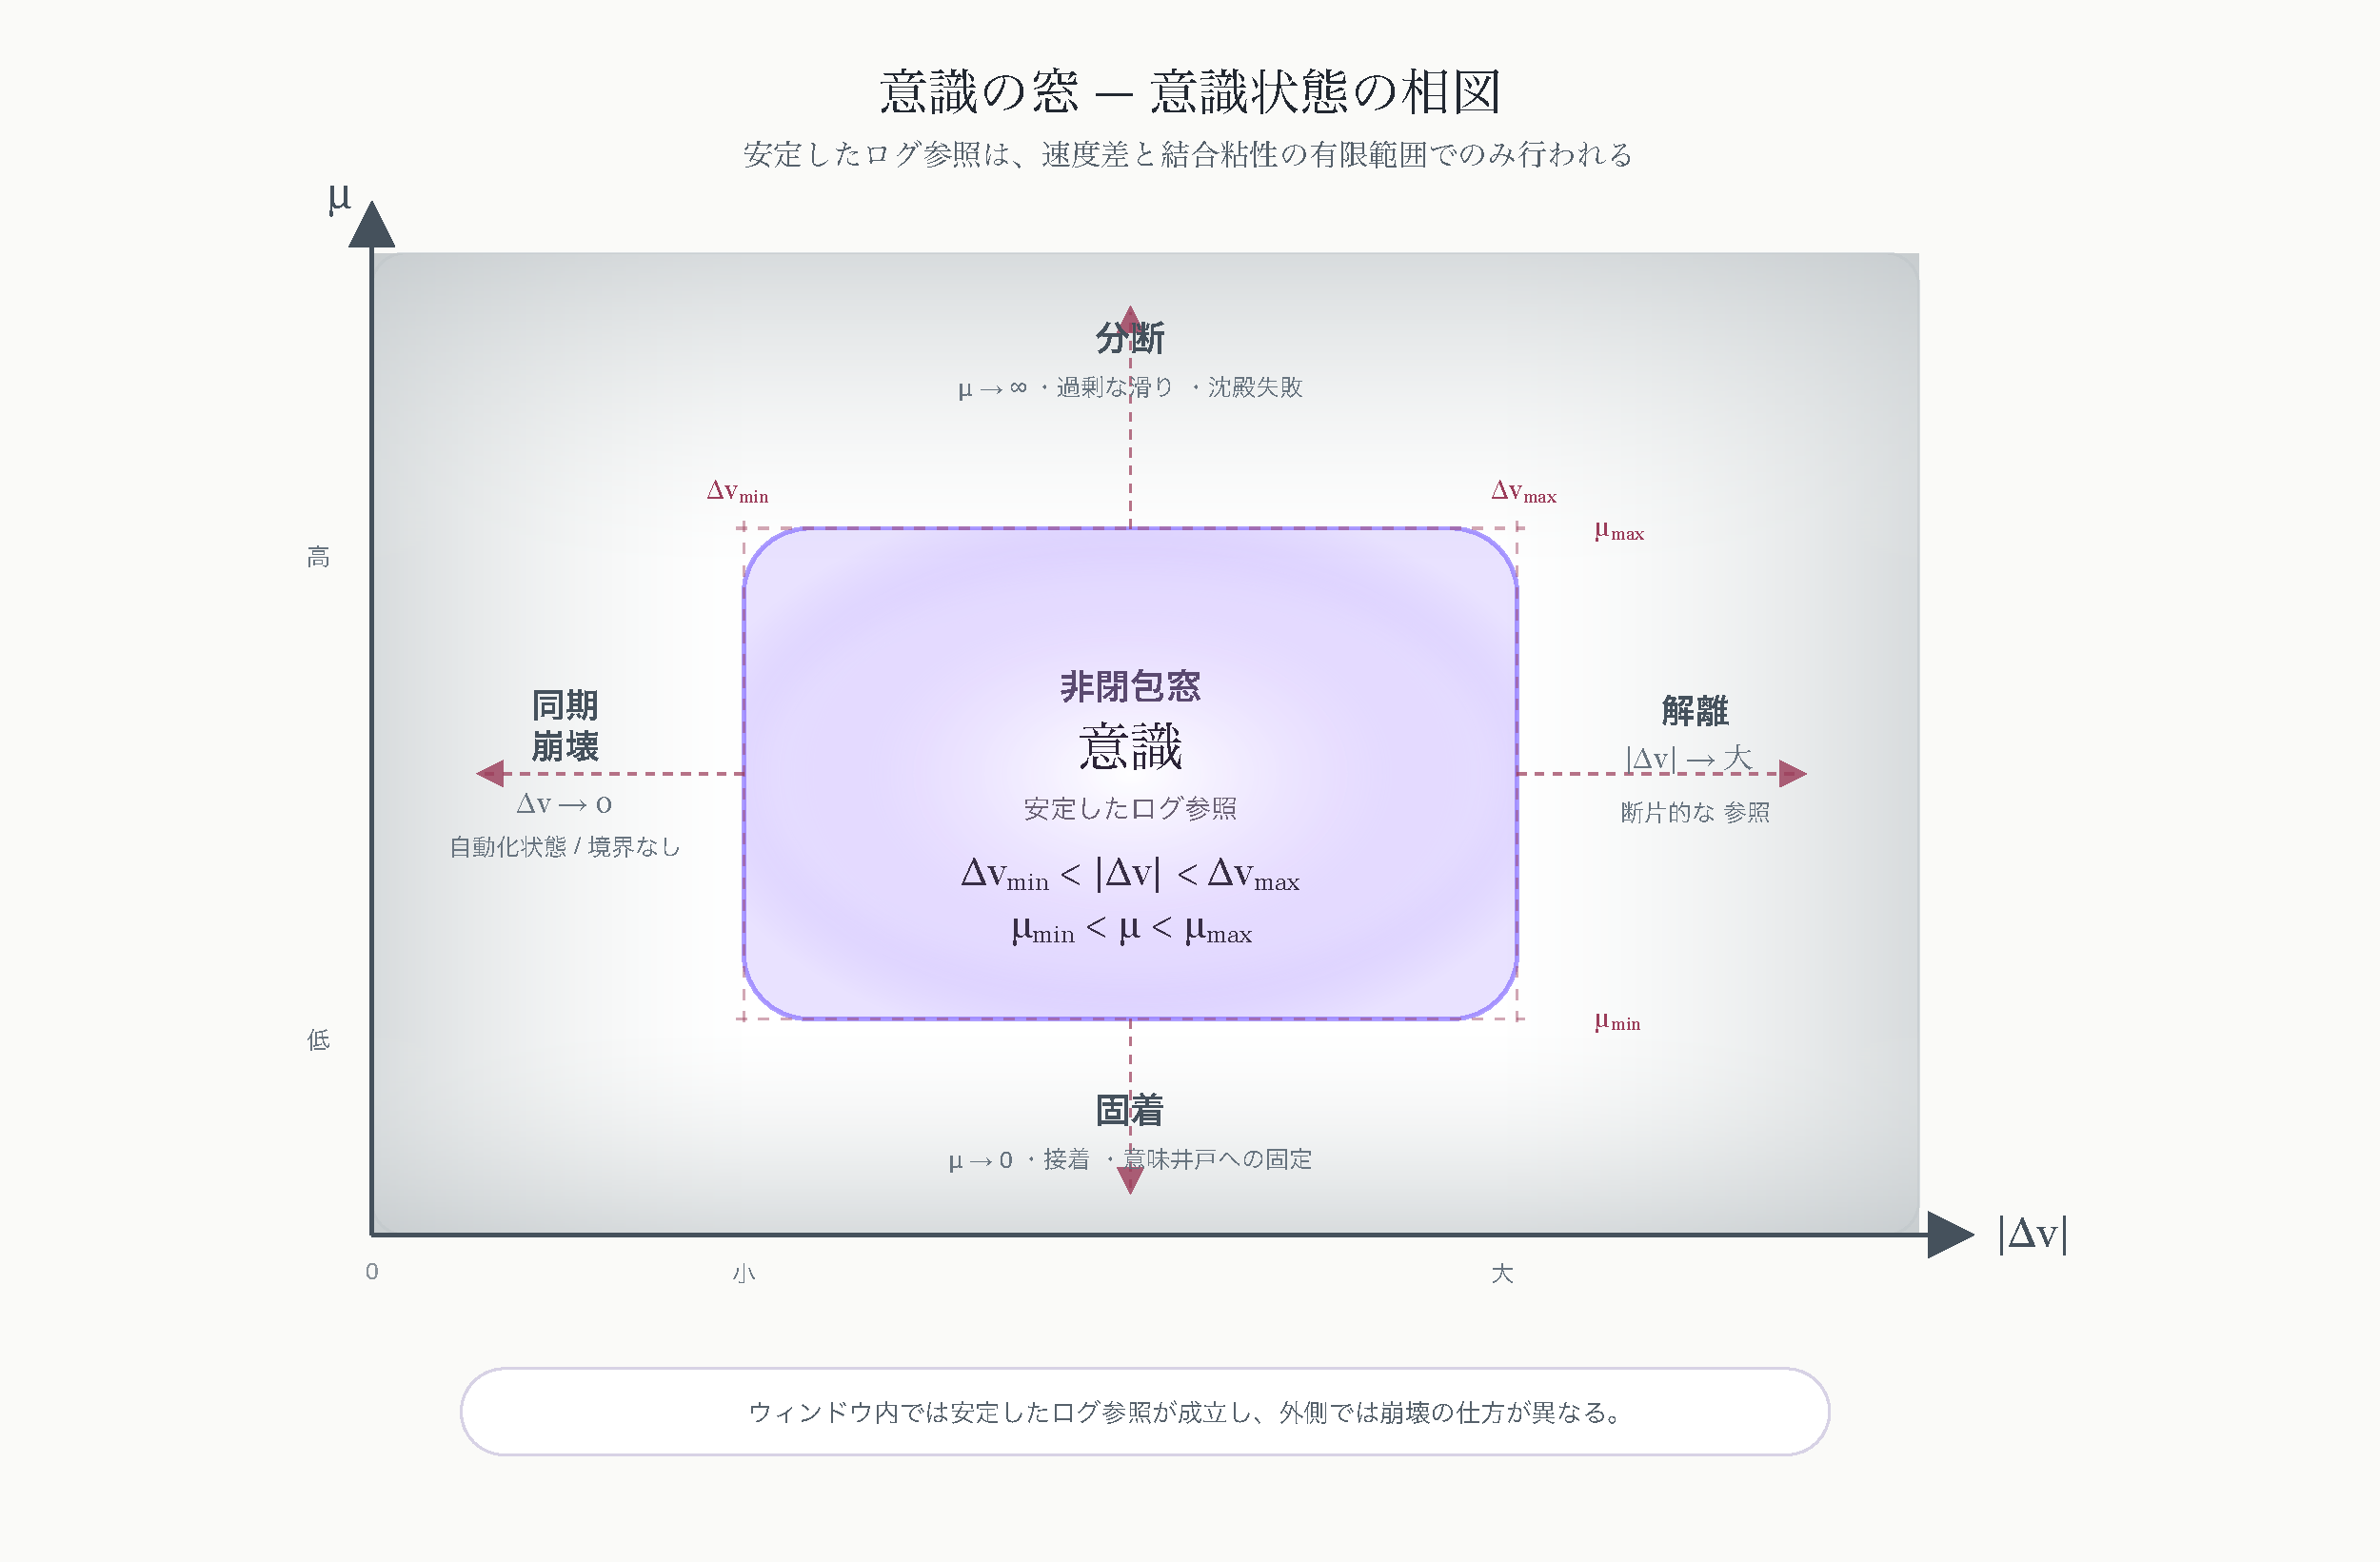
\includegraphics[width=0.86\linewidth]{figures_ja/figure3_nonclosure_window_jp.pdf}
\caption{
二軸の非閉包相図としての consciousness window。
安定したログ参照は、速度差と結合粘性が有限の範囲にあるときにのみ成立する。
この窓の外側では、システムは同期崩壊、解離、断片化、固着へ向かう。
}
\label{fig:consciousness-window-ja}
\end{figure}

\subsection{Non-Closure Condition}

VED の観点から見れば、意識は完全閉包ではなく、非閉包状態として維持される。

完全閉包とは、差が消え、流れが停止し、構造が通常の生成状態として維持できなくなる境界表現である。

意識はそのような状態ではない。

意識は、差が残り、流れがあり、しかし破綻しない範囲で維持される動的状態である。

したがって、意識の最小条件は次のように書ける。

\begin{equation}
\Delta v \neq 0,
\qquad
\nabla \Phi \neq 0,
\qquad
\frac{\partial I}{\partial t} \neq 0
\end{equation}

これは、意識が常に大きく揺らいでいる必要があるという意味ではない。

完全な静止、完全な同期、完全な閉包では意識状態が維持されないという意味である。

意識とは、閉じ切らない時間構造の中で、ログが参照可能になっている状態である。

VED の言語では、この非閉包条件は閉包度差 $\Delta C = C_s - C_f$ によって $0 < \Delta C < \Delta C_{\max}$ と等価に表現される（完全な写像は §6.4 を参照）。速度差と閉包度差という二つの記述は、同じ構造的条件を異なる座標で表したものであり、どちらか一方が他方を基礎づけるのではない。

\subsection{Summary}

本節で提示した式は、意識を生成する式ではない。

それらは、意識が成立しうる条件を制約する。

本稿の立場を最小限にまとめれば、次のようになる。

\begin{equation}
\text{Consciousness}
\;\sim\;
\text{Log Referencing}
\left(
\Delta v,
\mu,
\tau,
\mathcal{T}_{\Phi},
\nabla \Phi
\right)
\end{equation}

より直観的には、意識は次の条件で開かれる。

\begin{itemize}
\item 速度差があること。
\item 結合が切れていないこと。
\item 遅延が保持されていること。
\item 意味勾配が存在すること。
\item 完全閉包に至っていないこと。
\end{itemize}

この意味で、意識は生成物ではない。

意識は、時間差、粘性、意味勾配、非閉包が同時に成立したときに開かれるログ参照状態である。


\section{Structural Interpretation}


前節では、意識が成立しうる有効領域を、速度差、結合粘性、内部遅延、有効トルク様量、意味勾配によって整理した。

本節では、それらの式が何を意味しているのかを構造的に解釈する。

ここで重要なのは、前節の式が意識を生成する式ではないという点である。

それらは、意識という対象を計算するための式ではなく、意識がどのような条件のもとで開かれうるかを示す制約条件である。

\subsection{Consciousness Is Not an Object}

本稿の立場では、意識は内部に存在する対象ではない。

それは、脳内のどこかに置かれた部品でも、記憶の中に保存された内容でも、計算処理の最終出力でもない。

意識を対象として扱うと、ただちに次の問いが生じる。

どこにあるのか。

どの回路が作るのか。

どの情報量に対応するのか。

どれだけ生成されるのか。

しかし、前節で示したように、意識は単一変数に還元されない。

意識は、$I$、$J_I$、$J_{\log}$、$\Phi$、$\Delta v$、$\mu$、$\tau$、$\mathcal{T}_{\Phi}$ のいずれか一つではない。

それは、これらの関係が一定の有効領域に入ったときに開かれる状態である。

したがって、意識は object ではなく regime である。

それは、場所ではなく状態領域であり、産物ではなく条件である。

\subsection{Consciousness as a Window}

前節で導入した consciousness window は、意識を点ではなく窓として捉えるための概念である。

\begin{equation}
0 < |\Delta v| < \Delta v_{\max}
\end{equation}

\begin{equation}
\mu_{\min} < \mu < \mu_{\max}
\end{equation}

\begin{equation}
\tau_{\min} < \tau < \tau_{\max}
\end{equation}

\begin{equation}
\mathcal{T}_{\min}
<
\mathcal{T}_{\Phi}
<
\mathcal{T}_{\max}
\end{equation}

この窓の内側では、高速層と低速層は完全には同期しない。

同時に、完全にも分離しない。

処理は流れ去らず、しかし固定されすぎもしない。

ログは沈殿しうるが、完全閉包には至らない。

この中間領域において、現在処理と過去ログのあいだに参照関係が開かれる。

これが、本稿でいう意識状態である。

したがって、意識は ON/OFF の二値ではない。

意識は、consciousness window の内部で安定度、明瞭度、連続性、方向性を変えながら維持される動的状態である。

\subsection{Why Generation Is a Misleading Term}

意識を「生成される」と言うとき、そこには暗黙の構図がある。

生成者があり、生成物があり、生成されたものがどこかに存在する。

この構図は、物体や表象や出力を扱う場合には有効である。

しかし、本稿の枠組みでは、意識はそのような対象ではない。

意識は、高速層、低速層、可塑性ゲート、意味ポテンシャル、速度差、結合粘性が一定の関係を満たしたときに開かれる。

それは、何かが新しく作られるというより、すでに存在する処理とログのあいだに参照可能性が開くことである。

したがって、本稿では意識を生成された対象としてモデル化しない。

意識は、開かれる。

この「開かれる」という表現は、詩的比喩ではない。

それは、ログ参照のための時間的通路が一時的に成立するという構造的記述である。

ゲートが閉じれば意識状態は消える。

しかしそれは、生成された対象が破壊されたからではない。

ログ参照を可能にしていた関係が失われたからである。

\subsection{Consciousness as Temporal Non-Closure}

VED の観点から見ると、意識は時間的非閉包として理解される。

完全同期すれば、速度差は消える。

完全分離すれば、流れは届かない。

完全固定すれば、可塑性は失われる。

完全流動化すれば、ログは沈殿しない。

意識は、これらの極のいずれにも属さない。

意識は、閉じようとするが閉じ切らず、流れようとするが流れ去らず、沈殿しようとするが固定されすぎない状態にある。

この状態を、時間的非閉包と呼ぶ。

ここで非閉包とは、不完全さではない。

むしろ、持続の条件である。

もし完全に閉じてしまえば、意識は対象として固定されるかもしれないが、その時点でライブな参照状態ではなくなる。

逆に、まったく閉じなければ、処理は痕跡を残さず流れ去る。

意識は、この二つの間にある。

すなわち、意識は完全閉包の失敗ではなく、非閉包の安定化である。

より正確には、意識は状態ではなく、非閉包の持続である。

\begin{equation}
\text{Consciousness is not a state, but a sustained non-closure.}
\end{equation}

\subsection{Meaning Gradient and Selective Referencing}

IFGT の観点から見ると、意識は単なる時間構造ではない。

ログ参照は、意味勾配によって方向づけられる。

情報ポテンシャル $\Phi$ が形成されている領域では、処理はその勾配に沿って特定のログへ引き寄せられる。

\begin{equation}
|\nabla \Phi| \uparrow
\quad \Rightarrow \quad
\text{referencing bias} \uparrow
\end{equation}

このため、意識に現れるものはランダムではない。

強い記憶、感情的に重い出来事、繰り返し参照された概念、物語としてまとまったログは、意識的参照に入りやすい。

ただし、意味勾配が強いことは、意識が強いことと同義ではない。

意味勾配が過剰であれば、参照は特定の井戸へ固定される。

意味勾配が弱すぎれば、参照は方向を失う。

したがって、意識に必要なのは、意味勾配そのものではなく、速度差と粘性の範囲内で働く意味勾配である。

この点で、$\mathcal{T}_{\Phi}$ は重要である。

\begin{equation}
\mathcal{T}_{\Phi}
\sim
\kappa
\frac{\Delta v}{\mu}
|\nabla \Phi|
\end{equation}

この量は、何が意識に現れるかを単独で決めるものではない。

しかし、どのログが参照されやすくなるか、どの意味井戸へ処理が流れ込みやすいかを示す構造的指標である。

\subsection{Ego as a Derived Position}

この構造の中で、自我はどこに位置づくのか。

本稿の立場では、自我は意識の主体ではない。

それは、意識を所有する者でも、判断を下す中心でもない。

自我とは、高速層と低速層の速度差が、トルクコンバータ・アテンションによって変換される位置である。

この位置では、現在処理と過去ログが交差する。

行動準備、記憶沈殿、意味勾配、報告可能性が同時に重なる。

人間はこの交差点を、自分が考えている場所、自分が選んでいる場所、自分が意識している場所として経験しやすい。

しかし、それは自我が原因であることを意味しない。

自我は生成者ではなく、変換点である。

したがって、自我は幻想ではない。

それは機能的に実在する。

ただし、それは主体として実在するのではない。

時間スケール差の変換点として実在する。

\subsection{Qualia as Boundary Signal}

クオリアもまた、この構造の中で再配置される。

クオリアは意識の本体ではない。

それは、高速層の処理が低速層へ沈殿しようとする境界で現れるライブな前景である。

高速層に留まっているだけなら、クオリアはまだ報告可能な形にならない。

低速層へ完全に沈殿すれば、それは記憶、ラベル、報告、概念となる。

クオリアは、その中間にある。

したがって、クオリアは保存されない。

保存されるのは、クオリアが通過した後のログ構造である。

この見方では、クオリアは神秘的な実体ではない。

しかし、単なる錯覚でもない。

それは、ログ参照が開かれつつある境界の現象的側面である。

\subsection{Summary}

本節の構造的解釈をまとめると、次のようになる。

\begin{itemize}
\item 意識は対象ではなく、状態領域である。
\item 意識は生成された対象としてモデル化されず、ログ参照として開かれる。
\item 意識は完全閉包ではなく、時間的非閉包として維持される。
\item 意識に現れる内容は、意味勾配 $\nabla \Phi$ によって方向づけられる。
\item 自我は主体ではなく、速度差の変換点である。
\item クオリアは本体ではなく、沈殿境界のライブな前景である。
\end{itemize}

したがって、本稿における意識の構造的解釈は次の一文に集約される。

意識とは、意味勾配に方向づけられたログ参照が、完全同期にも完全分離にも至らない時間的非閉包レジームの中で開かれている状態である。

次節では、この構造が実際にどのように動くのかを、ログ参照のダイナミクスとして整理する。


\section{Dynamics of Log Referencing}


前節では、意識を対象ではなく、時間的非閉包レジームの中で開かれるログ参照状態として解釈した。

本節では、そのログ参照がどのような動的過程として成立するのかを整理する。

ここで扱うのは、意識がどこかで生成される過程ではない。

高速な処理が走り、低速なログが存在し、可塑性ゲートが開閉し、意味勾配が参照方向を偏らせる。その結果として、現在処理と過去ログのあいだに一時的な参照関係が開かれる。

この開口が、意識状態である。

\subsection{Fast Dynamics: Prediction Before Reference}

最初にあるのは、高速層の処理である。

高速層は、入力に対して即座に反応し、予測を生成し、行動候補を立ち上げる。

この処理は、まだ意識ではない。

それは速く、揮発的であり、多くの場合、そのまま消えていく。

高速層では、現在に対して未来が先取りされる。

何が起きそうか。

どの行動が可能か。

どの誤差を修正すべきか。

これらは、低速層に沈殿する前に、すでに部分的に走り始めている。

この意味で、行動準備や予測は、意識より先に現れることがある。

しかし、それは意識が無力であることを意味しない。

それは単に、高速層がログ参照より前の時間スケールで動いていることを意味する。

\subsection{Slow Dynamics: Sedimentation of Logs}

低速層は、高速層とは異なる時間構造を持つ。

低速層は、即時反応ではなく、沈殿、安定化、再参照可能性を担う。

ここでいうログとは、単なる記憶内容ではない。

ログとは、過去の処理が、後から参照可能な形で低速層に沈殿した構造である。

行為の系列、感情の痕跡、概念の配置、言語的ラベル、身体的反応の履歴。

これらはすべて、低速層におけるログ構造として残りうる。

しかし、ログが存在することと、意識されていることは同じではない。

ログは沈殿していても、現在処理から参照されていなければ、意識には現れない。

したがって、低速層は意識の本体ではない。

それは、意識が開かれるための参照可能な地形である。

\begin{quote}
\textbf{CT との対応（Conceptual Topography §6.1）：} 概念地形論では、このログ沈殿プロセスを「Sedimentation」と呼ぶ。新規入力$\Delta$が$\sigma_{\text{drive}}$スパイクを生成し、局所的に$I$が高まり、繰り返し参照によって$\Phi$のポテンシャル井戸が深化していく三段階（初期摂動→強化→安定化）が定式化されている。本稿の「ログが低速層に沈殿し再参照可能になる」という記述は、CTでは$\Phi \xrightarrow{\tau\to\infty} \Phi^*$という漸近的地形形成として書かれている。CTを読むと、ログ沈殿が単なる記憶保存ではなく場の幾何学的変形であることが見えてくる。
\end{quote}

\subsection{The Plasticity Gate}

高速層と低速層のあいだには、可塑性ゲートがある。

このゲートは、何を意識するかを選ぶスイッチではない。

それは、高速層の活動が低速層へ沈殿しうるかどうか、また低速層のログが現在処理へどの程度影響を与えるかを調整する時間的条件である。

ゲートが閉じすぎていれば、高速層の処理は低速層へ届かない。

この場合、処理は走っていても、経験として残らない。

逆に、ゲートが開きすぎていれば、高速層の変動が過剰に低速層へ書き込まれ、システムは硬直しやすくなる。

必要なのは、完全な開放でも完全な閉鎖でもない。

高速層の一部だけが、適切な遅延と粘性を伴って低速層へ沈殿することである。

この条件のもとで、ログ参照の可能性が開かれる。

\subsection{Delay as Thickness of Reference}

ログ参照には遅延が必要である。

この内部遅延を $\tau$ と表す。

\begin{equation}
\tau \propto \frac{\Delta v}{\mu}
\end{equation}

この遅延は、単なる処理の遅さではない。

それは、現在処理が低速層へ沈殿し、過去ログと重なり、再参照可能な構造へ変換されるための時間的厚みである。

もし $\tau$ がほとんどなければ、処理は即時反応として流れ去る。

そこには参照可能な厚みが生まれない。

逆に、$\tau$ が大きすぎれば、現在処理と沈殿したログの対応が崩れる。

この場合、意識状態は遅れ、断片化し、自己連続性を失いやすくなる。

したがって、ログ参照は遅延によって妨げられるのではない。

ログ参照は、適切な遅延によって可能になる。

\subsection{Meaning Gradient and Referencing Direction}

どのログが参照されるかは、単なる速度差だけでは決まらない。

ログ参照は、情報ポテンシャル $\Phi$ の勾配によって方向づけられる。

\begin{equation}
F = -\nabla \Phi
\end{equation}

意味勾配が強い領域では、現在処理はその方向へ引き寄せられやすい。

過去に何度も参照されたログ。

感情的に重いログ。

言語によって強く圧縮された概念。

反復された物語。

これらは、情報空間の中に意味井戸を形成し、現在処理を引き寄せる。

このとき、ログ参照は単なる想起ではない。

現在処理が、意味ポテンシャルの地形に沿って低速層へ接続される出来事である。

したがって、意識に現れる内容はランダムではない。

それは、速度差、結合粘性、遅延、意味勾配の相互作用によって偏る。

\begin{quote}
\textbf{CT との対応（Conceptual Topography §4.4）：} 概念地形論では、概念を「$\nabla\Phi(x)\approx 0$かつ小摂動に対して安定な$\Phi$の局所領域」として定義する。本稿の「意味井戸が現在処理を引き寄せる」という記述は、CTでは情報流$J_I = -D\nabla I + \mu F_I$が$-\nabla\Phi$に沿って低コスト領域へ引き込まれる力学として定式化されている。本稿でログ参照の方向を決める意味勾配$\nabla\Phi$は、CTで概念の深さ・幅・堅牢性を規定する同一の量である。CTを読むと、意識に現れる内容の偏りが概念地形の幾何学として読み替えられる。
\end{quote}

\subsection{Effective Referencing Torque}

速度差と意味勾配が結合すると、ログ参照には方向づけられた変換負荷が生じる。

これを、有効トルク様量 $\mathcal{T}_{\Phi}$ と表す。

\begin{equation}
\mathcal{T}_{\Phi}
\sim
\kappa
\frac{\Delta v}{\mu}
|\nabla \Phi|
\end{equation}

この量は、意識を生成する力ではない。

それは、現在処理がどの程度強く、どの方向へ、低速層のログへ接続されやすいかを示す構造的指標である。

$\mathcal{T}_{\Phi}$ が小さすぎれば、参照は開かれにくい。

処理は走っていても、意味方向を持たず、ログとして沈殿しにくい。

$\mathcal{T}_{\Phi}$ が大きすぎれば、参照は特定の意味井戸へ過剰に引き込まれる。

この場合、意識内容は明瞭になるかもしれないが、可塑性は低下する。

したがって、安定したログ参照には中間領域が必要である。

\begin{equation}
\mathcal{T}_{\min}
<
\mathcal{T}_{\Phi}
<
\mathcal{T}_{\max}
\end{equation}

この範囲内で、意識状態は安定して開かれる。

\subsection{The Referencing Loop}

ログ参照は一方向の流れではない。

高速層から低速層へ処理が沈殿するだけではなく、低速層のログは次の高速処理を制約する。

このループは次のように表せる。

\begin{enumerate}
\item 高速層が予測・反応・行動候補を生成する。
\item 可塑性ゲートを通過した一部の処理が低速層へ沈殿する。
\item 沈殿したログが情報密度 $I$ を変化させる。
\item 情報密度の配置が情報ポテンシャル $\Phi$ を変化させる。
\item $\nabla \Phi$ が次のログ参照と高速処理の方向を偏らせる。
\item その偏りのもとで、新たな高速処理が生じる。
\end{enumerate}

\cref{fig:log-loop-ja} は、ログ参照ループをまとめたものである。

\begin{figure}[H]
\centering
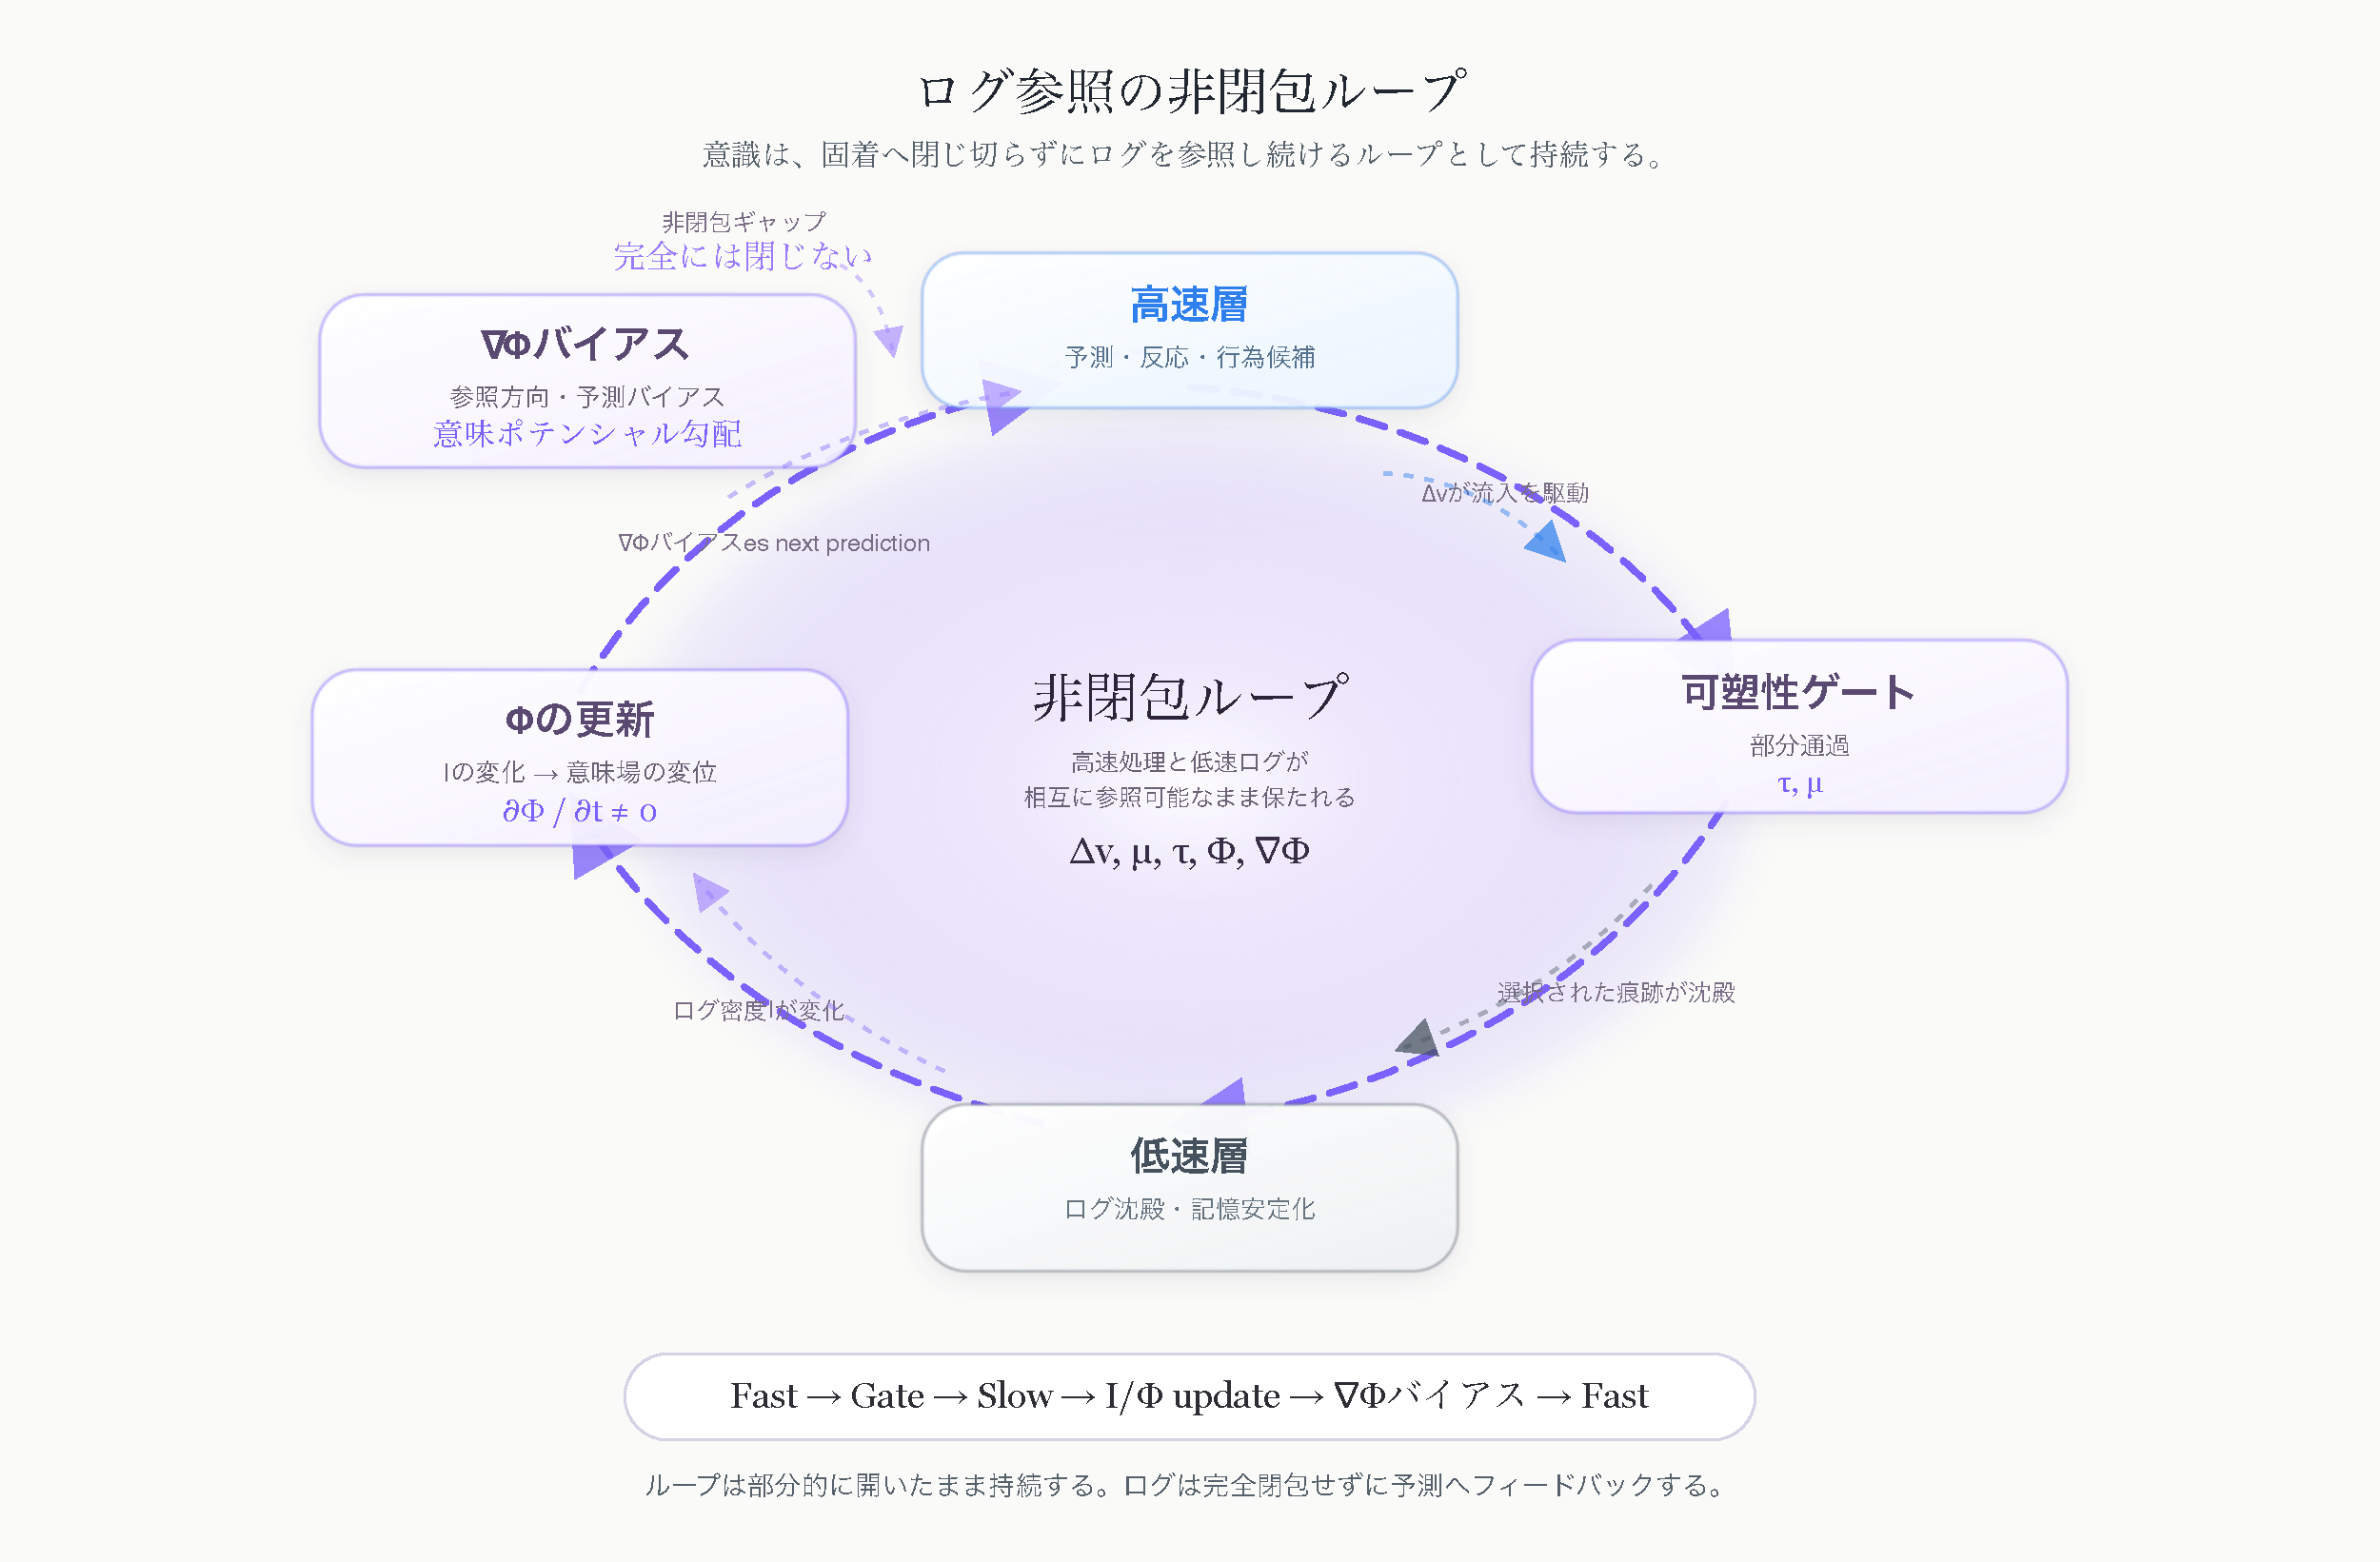
\includegraphics[width=0.92\linewidth]{figures_ja/figure4_log_referencing_loop_jp.pdf}
\caption{
ログ参照の非閉包ループ。
高速処理は、可塑性ゲートを部分的に通過して低速ログ沈殿へ向かう。
ログ密度の変化は意味ポテンシャルを更新し、その勾配が次の予測を偏らせる。
このループは、部分的に開かれたまま維持されることで持続する。
}
\label{fig:log-loop-ja}
\end{figure}

このループにより、意識状態は単なる瞬間的出来事ではなく、時間をまたいで持続する構造になる。

ただし、このループは完全には閉じない。

完全に閉じれば、処理は固定され、可塑性を失う。

完全に開けば、処理は沈殿せず、ログ参照は成立しない。

したがって、ログ参照ループは非閉包的に維持される。

この非閉包性こそが、意識状態の持続条件である。

\subsection{Conscious Access and Report}

意識状態と報告可能性は同一ではない。

しかし、本稿の枠組みでは、両者は密接に関係する。

報告とは、低速層に沈殿したログが、言語や行動を通じて外部化可能になることである。

そのため、処理が起きていても、それが低速層へ沈殿しなければ報告できない。

また、沈殿していても、報告経路へ接続されなければ明示的には語れない。

Libet 型実験では、行動準備と報告可能なタイムスタンプの時間差が問題になる。

分離脳実験では、処理と報告経路の空間的切断が問題になる。

どちらの場合も、問題は意識が存在するかどうかではなく、処理がログ参照と報告可能性の経路へどのように接続されるかである。

\subsection{Non-Closure of the Loop}

ログ参照ループは、安定しているほどよいわけではない。

安定しすぎれば、固定化する。

不安定すぎれば、断片化する。

したがって、意識状態に必要なのは、閉じたループではなく、閉じ切らないループである。

この構造は、VED の非閉包原理と対応する。

差があり、勾配が立ち、流れが生じ、構造は閉じようとする。

しかし完全には閉じない。

意識状態も同じである。

現在処理はログへ沈殿しようとする。

ログは現在処理を制約しようとする。

意味場は参照を方向づけようとする。

しかし、すべてが完全に固定されることはない。

この未完のループが、意識状態を維持する。

\subsection{Summary}

本節では、ログ参照の動的過程を整理した。

意識は、高速層、低速層、可塑性ゲート、内部遅延、意味勾配、有効トルク様量が形成する非閉包ループとして理解される。

このループにおいて、

\begin{itemize}
\item 高速層は未来を先取りする。
\item 低速層は過去を沈殿させる。
\item 可塑性ゲートは何が沈殿するかを調整する。
\item 内部遅延 $\tau$ は参照の時間的厚みを与える。
\item 意味勾配 $\nabla \Phi$ は参照方向を偏らせる。
\item $\mathcal{T}_{\Phi}$ は速度差と意味勾配が結合した参照負荷を表す。
\item 非閉包性はループの持続条件である。
\end{itemize}

したがって、意識とは、ログが保存されていることではない。

また、処理が走っていることでもない。

意識とは、高速処理と低速ログが、意味勾配に沿って、閉じ切らないループの中で相互参照可能になっている状態である。


\section{Experimental Reinterpretation}


本節では、前節までに定式化したログ参照モデルを用いて、既存の代表的な意識実験を再解釈する。

ここで行うのは、実験結果の否定ではない。

むしろ、既存実験が示していたものを、意識生成モデルではなく、時間スケール間のログ参照モデルとして読み直すことである。

意識研究における多くの混乱は、処理、行動、報告、意識を単一の時間軸上に並べてしまうことから生じている。

この見方では、早く現れたものが原因であり、遅く現れたものは結果であると解釈されやすい。

しかし、本稿の枠組みでは、システムは単一の時計で動いていない。

高速層は予測し、低速層は沈殿し、可塑性ゲートは両者の間に遅延と粘性を導入する。

したがって、実験で観測される時間差や報告不能性は、意識の欠如を意味するとは限らない。

それらは、処理がログ参照可能な状態へ到達するまでの、時間的・経路的条件を示している。

\subsection{Libet-Type Experiments}

Libet 型実験では、被験者が任意のタイミングで手首や指を動かし、その際に「動かそうと思った瞬間」を報告する。

同時に、脳活動が測定される。

よく知られているように、運動に先立って準備電位が立ち上がり、その後で被験者の意識的な意図報告が現れる。

従来、この結果はしばしば次のように解釈されてきた。

脳が先に決め、意識は後からそれを知る。

あるいは、自由意志は幻想である。

しかし、この解釈は、決定、脳活動、意識報告を同一の時間軸上に置くことを前提としている。

本稿の枠組みでは、この前提を採らない。

準備電位は、高速層における行動候補の形成として読むことができる。

それは、未来志向の予測的・運動的ダイナミクスが、ある行動アトラクタへ落ち込み始めたことを示す信号である。

一方で、「いま動かそうと思った」という報告は、その高速処理が低速層のログ参照構造へ接続された後に現れる。

このとき初めて、処理は「自分がそうしようとしている」という報告可能な形式を取る。

したがって、Libet 型実験で観測される時間差は、意識の遅れではなく、速度スケール間の変換時間である。

高速層の処理速度を $v_f$、低速層の沈殿速度を $v_s$ とすれば、両者の速度差は次のように表される。

\begin{equation}
\Delta v = v_f - v_s
\end{equation}

この速度差は、内部遅延 $\tau$ として現れる。

\begin{equation}
\tau \propto \frac{\Delta v}{\mu}
\end{equation}

ここで $\mu$ は、高速層と低速層の結合粘性である。

つまり、Libet 型実験が測定したものは、自由意志の有無ではなく、高速な行動準備が低速な報告可能ログへ変換されるまでの遅延である。

この見方では、「意識は遅れている」という表現も十分ではない。

意識は、そもそも高速層と同じ時計で動いていない。

意識は、高速処理がログ参照可能な状態へ変換された地点で開かれる。

そのため、準備電位が先行することは、意識が無力であることを示さない。

それは、意識が行動準備そのものではなく、行動準備が低速層へ沈殿し、参照可能になる通過点であることを示している。

\subsection{Why Free Will Is Not the Proper Question Here}

Libet 型実験が繰り返し自由意志の議論へ引き込まれる理由は、「決定」が一点で起きるという前提にある。

しかし、本稿の構造では、決定は単一の時点に局在しない。

高速層では、複数の行動候補が予測的に立ち上がる。

可塑性ゲートは、その一部が低速層へ沈殿しうるかを調整する。

低速層では、過去ログ、意味勾配、身体状態、文脈が、報告可能な形式を作る。

この全体を一つの「決定点」に圧縮すると、時間構造が失われる。

そのため、Libet 型実験に対して「意識が決めたのか、脳が決めたのか」と問うことは、構造的には不適切である。

適切な問いは、次のようなものである。

どの処理が高速層で先行したのか。

その処理はどの程度の遅延 $\tau$ を経て低速層へ接続されたのか。

どのログが意味勾配 $\nabla \Phi$ によって参照されたのか。

どの時点で報告可能な形式が成立したのか。

このように問いを置き換えると、Libet 型実験は自由意志を否定する実験ではなく、単一時間軸モデルの限界を可視化した実験になる。

\subsection{Split-Brain Experiments}

分離脳実験では、脳梁を切断した患者において、左右半球の情報共有が制限される。

この状況で、右半球に提示された刺激に対して適切な行動反応が起きる一方で、その刺激を言語的に報告できない場合がある。

この現象は、しばしば「二つの意識」や「二つの自己」の証拠として語られてきた。

しかし、本稿の枠組みでは、この読みは過剰である。

分離脳実験が示しているのは、意識が二重化することではない。

それは、処理、沈殿、報告の経路が非対称化しうるということである。

右半球で処理が起きていても、その処理が左半球優位の言語報告経路へ到達しなければ、被験者はそれを明示的に語れない。

このとき、処理が存在しないわけではない。

行動反応が起きていることからも、局所的な処理は明らかに走っている。

しかし、その処理は報告可能な低速ログへ統合されていない。

したがって、分離脳実験で失われているのは、処理そのものではなく、参照経路である。

この点は、Libet 型実験と対応している。

Libet 型実験では、処理と報告の間に時間的遅延が現れる。

分離脳実験では、処理と報告の間に経路的断絶が現れる。

どちらも、処理が明示的意識になるためには、低速層へのログ沈殿と参照可能性が必要であることを示している。

\subsection{Reporting Bottleneck and Log Accessibility}

分離脳実験において特に重要なのは、報告可能性と意識を同一視しないことである。

報告可能性は、意識状態の一部を外部化する経路である。

しかし、報告できないことは、処理が起きていないことを意味しない。

本稿の枠組みでは、明示的報告には少なくとも三つの条件が必要である。

第一に、処理が高速層で生じていること。

第二に、その処理が低速層へ沈殿し、ログ参照可能になっていること。

第三に、そのログが言語または行動の報告経路へ接続されていること。

分離脳では、この第三の条件が非対称化する。

そのため、ある処理は行動として表出するが、言語報告としては現れない。

この非対称性を「二つの意識」と読む必要はない。

より正確には、ログ参照経路と報告経路の一部が切断されているのである。

\subsection{Rationalization as Log Completion}

分離脳実験でよく知られる現象として、左半球が、実際には参照できていない行動の理由を後から説明することがある。

これはしばしば「作話」や「合理化」と呼ばれる。

本稿の立場では、この合理化は意図的な虚偽ではない。

それは、欠落したログを補完し、低速層の一貫性を保とうとする自然な振る舞いである。

低速層は、参照可能なログを用いて自己の連続性を維持する。

しかし、処理経路が切断されている場合、行動は起きているのに、その行動を生んだログが参照できない。

このとき、システムは欠落をそのまま欠落として保持するより、参照可能なログからもっとも整合的な説明を生成する。

この合理化は、意識が嘘をついていることを示さない。

むしろ、意識が参照可能なログから一貫性を構成していることを示している。

この点で、分離脳実験は自我が主体であるという見方を弱める。

自我はすべてを知っている中心ではない。

それは、参照可能なログから自己連続性を組み立てる変換点である。

\subsection{Experimental Correspondence to the Model}

Libet 型実験と分離脳実験は、一見すると異なる問題を扱っている。

前者は時間差を扱い、後者は半球間の経路分断を扱う。

しかし、本稿の枠組みでは、両者は同じ構造の異なる断面である。

Libet 型実験は、次の関係を可視化している。

\begin{equation}
\text{fast preparation}
\rightarrow
\text{delayed sedimentation}
\rightarrow
\text{reportable timestamp}
\end{equation}

分離脳実験は、次の関係を可視化している。

\begin{equation}
\text{localized processing}
\rightarrow
\text{blocked transmission}
\rightarrow
\text{asymmetric reportability}
\end{equation}

どちらの場合も、処理そのものと意識報告は同一ではない。

処理は、可塑性ゲート、遅延、沈殿、報告経路を通過して初めて明示的意識として現れる。

この構造を用いれば、既存実験は次のように再配置される。

\begin{itemize}
\item Libet 型実験：速度スケール差と内部遅延 $\tau$ の露出。
\item 分離脳実験：ログ参照経路と報告経路の非対称化。
\item 合理化：参照不能ログの欠落に対する低速層の整合化。
\item 意識報告：処理そのものではなく、沈殿したログの外部化。
\end{itemize}

この再配置によって、意識は因果の源泉でも、単なる後付け幻想でもなくなる。

意識は、処理がログ参照可能な形へ変換されたときに開かれる状態である。

\subsection{What These Experiments Do Not Show}

最後に、これらの実験が示していないことを明確にしておく。

Libet 型実験は、自由意志が存在しないことを示したわけではない。

それは、行動準備と意識報告が異なる時間スケールで生じることを示した。

分離脳実験は、人間の内部に二つの自己が存在することを示したわけではない。

それは、処理経路と報告経路が切断されると、ログ参照が非対称化することを示した。

合理化は、意識が常に虚偽を語ることを示したわけではない。

それは、参照できないログの欠落を、低速層が一貫性のある形で補完することを示した。

したがって、これらの実験は意識を消し去るものではない。

むしろ、意識を正しい位置に戻す。

それは、行動の起点でも、脳内に生成される対象でもなく、速度スケール間のログ参照が報告可能な形に開かれた状態である。

\subsection{Summary}

本節では、Libet 型実験と分離脳実験を、本稿のログ参照モデルから再解釈した。

両者に共通するのは、処理と意識報告の非同一性である。

処理は走る。

しかし、それが低速層へ沈殿し、ログとして参照可能になり、報告経路へ接続されなければ、明示的意識としては現れない。

したがって、既存実験が示していたのは、意識の無力さではない。

それは、意識が成立するための時間的・経路的条件である。

次節では、このログ参照が沈殿境界でどのように現象的な前景を持つのか、すなわちクオリアを境界現象として位置づける。


\section{Qualia as Boundary Phenomenon}


本節では、クオリアを本稿の構造の中に位置づける。

ここで行うのは、クオリアを否定することではない。

また、クオリアを意識の中心に置くことでもない。

本稿の立場では、クオリアは意識そのものではない。

それは、ログ参照が開かれつつある境界で現れる、現象的な前景である。

\subsection{Why the Qualia Problem Does Not Converge}

クオリア問題は、長いあいだ意識研究の中心に置かれてきた。

赤の赤さ。

痛みの痛さ。

音の響き。

今ここにある感じ。

これらは、確かに経験される。

そのため、クオリアを否定することはできない。

しかし、クオリアを意識の本体として扱うと、議論は収束しにくくなる。

理由は単純である。

クオリアは、保存された対象ではないからである。

クオリアを「どこにあるのか」「何として保存されているのか」「どの表象に対応するのか」と問うと、問いは最初からずれる。

それは、流れている境界を、固定された物体として探すことに近い。

本稿では、クオリア問題が終わらない理由を、神秘性ではなく、位置づけの誤りとして捉える。

クオリアは、内部に存在する何かではない。

それは、処理がログとして沈殿しつつある境界で、一時的に現れる現象である。

\subsection{Qualia as Sedimentation Frontier}

本稿では、クオリアを沈殿前線として位置づける。

高速層では、予測、反応、誤差、行動候補が揮発的に走る。

低速層では、それらの一部がログとして沈殿し、再参照可能な構造になる。

クオリアは、この二つの層のどちらか一方に属するものではない。

それは、高速層の処理が低速層へ沈殿しようとする境界に現れる。

この境界を、沈殿前線、または closure frontier と呼ぶことができる。

ここでいう closure は、完全閉包を意味しない。

処理が完全に閉じてしまえば、それはすでにログ、記憶、ラベル、概念になっている。

一方で、まったく閉じなければ、処理は痕跡を残さず流れ去る。

クオリアは、その中間にある。

閉じようとしているが、まだ閉じ切っていない。

流れているが、すでに沈殿へ向かっている。

この過渡状態が、クオリアとして経験される。

\cref{fig:qualia-boundary-ja} は、クオリアを一時的な境界状態として位置づける。

\begin{figure}[H]
\centering
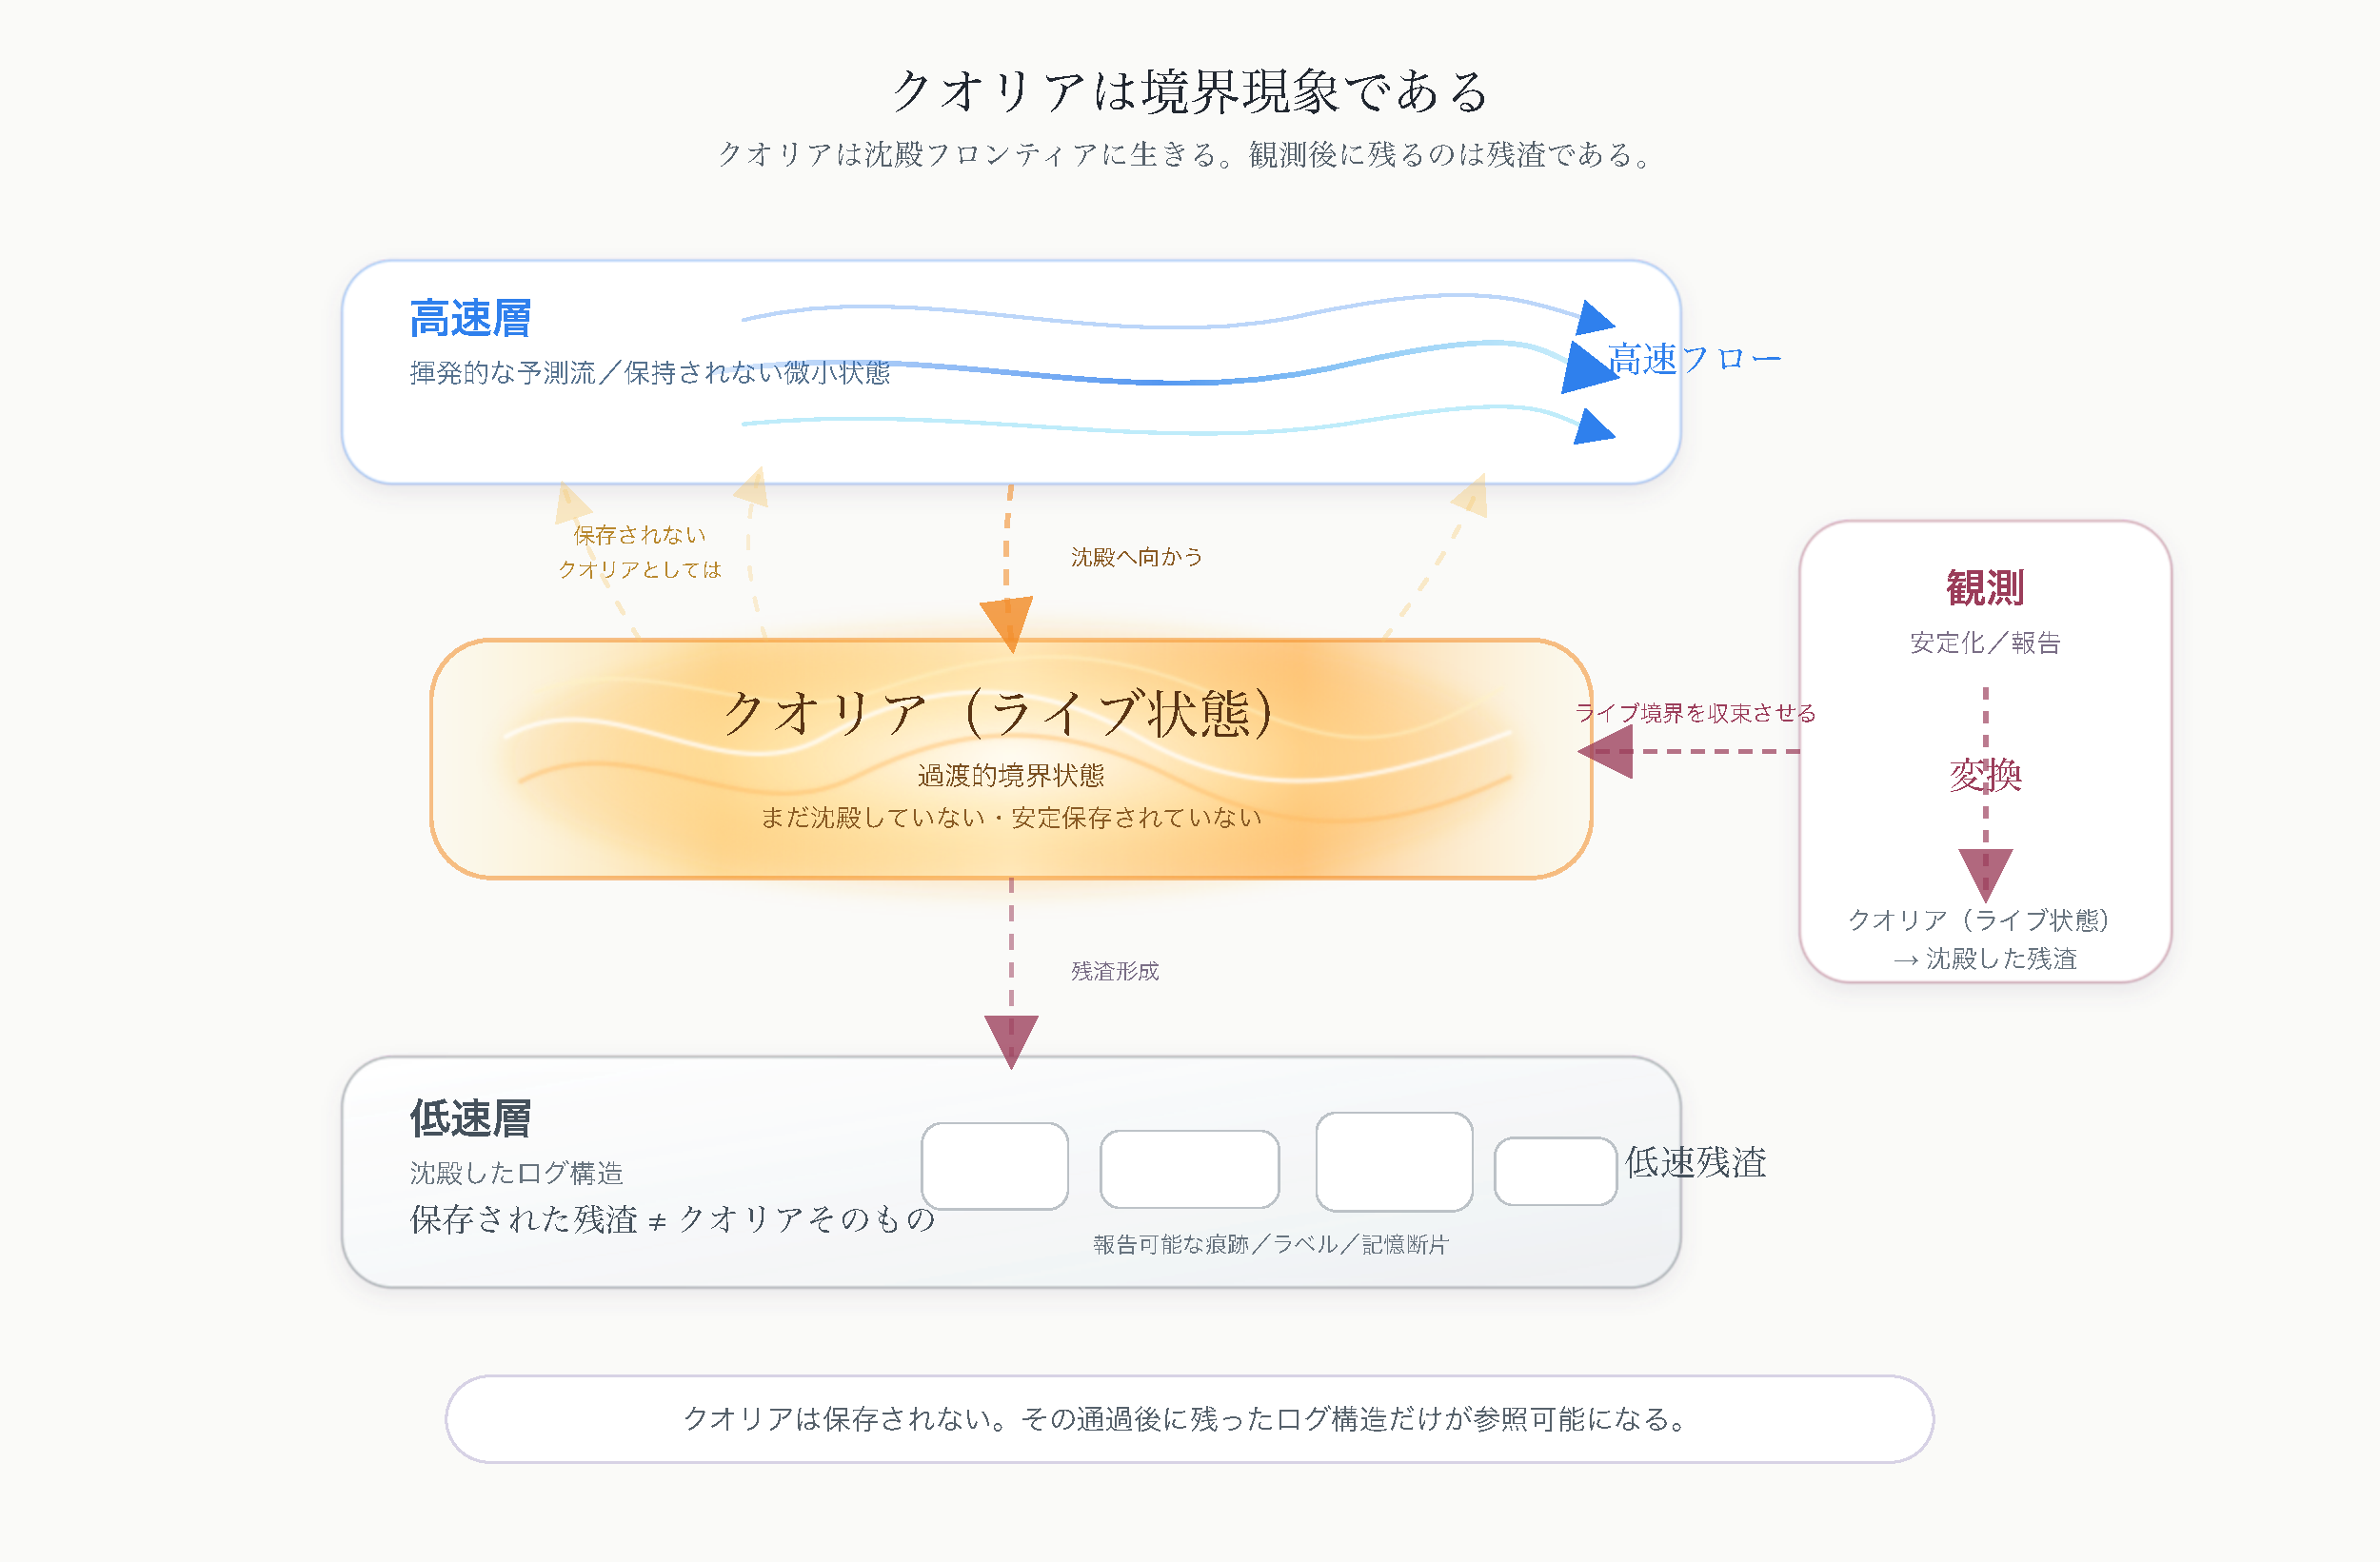
\includegraphics[width=0.92\linewidth]{figures_ja/figure5_qualia_boundary_jp.pdf}
\caption{
境界現象としてのクオリア。
クオリアは、高速な予測流と低速なログ構造のあいだの沈殿前線にライブに現れる。
測定はこのライブな境界を安定化し、沈殿残余へ変換する。
再参照可能なものとして残るのはクオリアそのものではなく、その通過後に残されたログ構造である。
}
\label{fig:qualia-boundary-ja}
\end{figure}

\subsection{Qualia Are Live, Not Stored}

クオリアは保存されない。

この言い方は強く見えるかもしれない。

しかし、ここで意味しているのは、クオリアが存在しないということではない。

クオリアは存在する。

ただし、それは保存物として存在するのではなく、ライブな境界状態として存在する。

たとえば、痛みの記憶は残る。

赤を見たという記憶も残る。

音楽を聴いたという記憶も残る。

しかし、残っているのはクオリアそのものではない。

残っているのは、クオリアが通過した後のログ構造である。

記憶として再生されるものは、かつてのクオリアではなく、クオリアを伴って更新された低速層の痕跡である。

したがって、クオリアを忠実に保存しようとする試みは、構造的に失敗する。

保存された瞬間、それはすでにクオリアではなく、ログになっている。

\subsection{Qualia and the Plasticity Gate}

クオリアは、可塑性ゲートの近傍で現れる。

高速層の処理が低速層へ沈殿するためには、可塑性ゲートを通過しなければならない。

このゲートが完全に閉じていれば、処理は経験として残らない。

このゲートが完全に開きすぎていれば、処理は過剰に沈殿し、固定化しやすくなる。

クオリアは、そのゲートが開きつつあり、しかしまだ沈殿が完了していない状態に現れる。

したがって、クオリアはゲートの産物ではない。

それは、ゲートを通過しつつある処理の現象的側面である。

この意味で、クオリアはログ参照の結果でもあり、ログ沈殿の途中経過でもある。

完全に高速層側にあれば、まだ報告可能ではない。

完全に低速層側に入れば、すでに記憶や言語ラベルになっている。

クオリアは、その境界でだけライブに現れる。

\subsection{Qualia and Effective Torque}

クオリアの明瞭さは、単なる刺激の強度だけでは決まらない。

本稿の枠組みでは、クオリアは速度差、結合粘性、意味勾配の組み合わせによって変化する。

この関係は、有効トルク様量として次のように表される。

\begin{equation}
\mathcal{T}_{\Phi}
\sim
\kappa
\frac{\Delta v}{\mu}
|\nabla \Phi|
\end{equation}

$\mathcal{T}_{\Phi}$ が小さすぎる場合、処理は十分な参照方向を持たず、クオリアはぼんやりする。

$\mathcal{T}_{\Phi}$ が中間領域にある場合、処理は低速層へ沈殿しつつも、まだライブな境界として保たれる。

このとき、クオリアは明瞭でありながら、固定されすぎない。

一方で、$\mathcal{T}_{\Phi}$ が大きすぎる場合、処理は特定の意味井戸へ過剰に引き込まれる。

この場合、クオリアは強く感じられるかもしれない。

しかし、その強さは必ずしも自由な意識状態を意味しない。

むしろ、意味勾配が強すぎることで、クオリアが特定の記憶や物語へ固定されやすくなる。

したがって、クオリアの明瞭さと意識の安定性は同義ではない。

\subsection{Measurement Converts Qualia into Residue}

クオリアは測定によって変質する。

これは、クオリアが神秘的だからではない。

クオリアが境界現象だからである。

測定とは、対象を安定化し、報告可能にし、比較可能にする操作である。

しかし、クオリアは安定化される前の境界にある。

そのため、測定しようとすると、クオリアは低速層へ沈殿し、ログ、ラベル、報告、数値、神経的要約へと変換される。

測定後に残るものは、クオリアそのものではない。

それは、クオリアが通過した後の残余である。

この関係は次のように表せる。

\begin{equation}
\text{qualia live}
\rightarrow
\text{measurement}
\rightarrow
\text{sedimented residue}
\end{equation}

したがって、クオリアが測れないという主張は、「何も観測できない」という意味ではない。

観測できるのは、クオリアそのものではなく、クオリアが沈殿した後の痕跡である。

\subsection{Why Qualia Feel Central}

クオリアは意識の本体ではない。

しかし、体験上は非常に中心的に感じられる。

この理由は、クオリアがログ参照のライブな境界に現れるからである。

人間が「いま意識している」と感じる瞬間には、何らかの処理が沈殿しつつあり、同時にまだ完全にはログ化されていない。

その境界で、感覚は鮮明に現れる。

そのため、クオリアは原因であるかのように見える。

しかし、構造的には、クオリアは原因ではない。

それは、処理と沈殿の境界で観測される前景である。

光が物体の存在そのものではなく、物体と観測条件の関係として現れるように、クオリアもまた、処理とログ沈殿の関係として現れる。

このため、クオリアを中心に置くと意識は神秘化される。

しかし、クオリアを境界に置くと、意識はログ参照構造として読み直せる。

\subsection{Relation to the Hard Problem}

いわゆる hard problem は、クオリアを固定された説明対象として扱うところから生じる。

なぜこの神経活動が「この感じ」を伴うのか。

なぜ物理過程が主観的経験になるのか。

この問いは強力である。

しかし、本稿の立場では、この問いはクオリアを保存物として扱っている。

本稿では、クオリアを保存物ではなく、沈殿境界のライブな前景として扱う。

この場合、問うべきことは変わる。

「クオリアはどこにあるのか」ではない。

「どのような条件で、処理はログ化される直前の境界として経験されるのか」である。

この問いに対しては、速度差、結合粘性、内部遅延、意味勾配、可塑性ゲートという構造で答えることができる。

したがって、本稿は hard problem を解いたとは言わない。

むしろ、hard problem を、解けない対象問題から、記述可能な境界条件の問題へ移す。

\subsection{Summary}

本節では、クオリアを境界現象として位置づけた。

\begin{itemize}
\item クオリアは意識の本体ではない。
\item クオリアは保存された対象ではない。
\item クオリアは高速層と低速層の沈殿前線に現れる。
\item クオリアは可塑性ゲートの近傍でライブに成立する。
\item 測定はクオリアを残余へ変換する。
\item クオリアの明瞭さは、$\Delta v$、$\mu$、$\tau$、$\nabla \Phi$、$\mathcal{T}_{\Phi}$ に依存する。
\item hard problem は、クオリアを対象として探す限り収束しない。
\end{itemize}

したがって、クオリアとは、ログ参照が沈殿しつつある境界で現れる、非保存的なライブ前景である。

次節では、この境界現象を含めた意識全体を、生成モデルではなく opening model として整理する。


\section{Opening Model}


本節では、本稿の中心命題である「意識を生成された対象としてモデル化しない」という主張を、opening model として整理する。

ここでいう opening とは、比喩的な表現ではない。

それは、高速層、低速層、可塑性ゲート、意味勾配、内部遅延が一定の関係に入ったとき、ログ参照可能な通路が一時的に開かれるという構造的記述である。

意識は、内部に新しく作られる対象ではない。

意識は、すでに走っている処理と、すでに沈殿しているログとのあいだに、参照可能性が開かれた状態である。

\subsection{The Generation Assumption}

意識をめぐる多くの議論は、明示的または暗黙のうちに生成モデルを採っている。

生成モデルでは、意識は何らかの処理によって作られるものとして扱われる。

この見方では、自然に次の問いが生じる。

どの脳部位が意識を生成するのか。

どの回路が意識を作るのか。

どの計算量が意識を生むのか。

意識はどれだけ生成されるのか。

生成された意識は保存できるのか、コピーできるのか。

これらの問いは、一見すると自然である。

しかし、それらはすべて、意識を産物として扱う前提を含んでいる。

生成者があり、生成過程があり、生成された対象がある。

この三項構造が、生成モデルの基本である。

本稿では、この前提を採らない。

本稿では、意識を処理の産物として扱わない。意識は、処理とログの関係がある時間的条件に入ったときに開かれる状態である。

\subsection{From Product to Relation}

生成モデルでは、意識は product として扱われる。

しかし、本稿では、意識を relation として扱う。

すなわち、意識とは、高速な予測処理と低速なログ沈殿のあいだに成立する参照関係である。

この関係が成立するためには、少なくとも次の条件が必要である。

\begin{enumerate}
\item 高速層において処理が走っていること。
\item 低速層に参照可能なログが沈殿していること。
\item 両者のあいだに有限の速度差 $\Delta v$ があること。
\item 結合粘性 $\mu$ が、完全同期と完全分離の中間にあること。
\item 内部遅延 $\tau$ が、参照可能な厚みとして保持されていること。
\item 意味勾配 $\nabla \Phi$ が、参照方向を与えていること。
\item 有効トルク様量 $\mathcal{T}_{\Phi}$ が、consciousness window の範囲内にあること。
\end{enumerate}

この条件がそろったとき、意識が「作られる」のではない。

ログ参照が開かれる。

したがって、意識は出力ではなく、関係の開口である。

\subsection{Opening Through the Plasticity Gate}

opening model において中心的な役割を持つのが、可塑性ゲートである。

可塑性ゲートは、意識を作る装置ではない。

それは、高速層の処理が低速層へ沈殿しうるか、また低速層のログが現在処理へどの程度影響を及ぼすかを調整する境界条件である。

ゲートが完全に閉じていれば、処理は低速層へ届かない。

この場合、処理は走っていても、ログ参照は開かれない。

ゲートが完全に開きすぎていれば、処理は過剰に沈殿し、可塑性を失いやすい。

この場合、意識は自由に開かれるというより、特定のログや意味井戸へ固定されやすくなる。

opening model が必要とするのは、完全な開放ではない。

むしろ、部分的で一時的な開口である。

この開口は、速度差、結合粘性、内部遅延、意味勾配によって調整される。

\begin{equation}
\mathcal{T}_{\Phi}
\sim
\kappa
\frac{\Delta v}{\mu}
|\nabla \Phi|
\end{equation}

$\mathcal{T}_{\Phi}$ が consciousness window の範囲内にあるとき、ゲートはログ参照に適した形で開かれる。

このとき、意識状態が成立する。

\subsection{Consciousness Opens, Qualia Appear}

前節で見たように、クオリアはログ参照が沈殿しつつある境界で現れるライブな前景である。

opening model では、クオリアもまた生成物ではない。

クオリアは、意識が開かれたときに、その境界で現れる現象的側面である。

意識が開かれるとは、高速層と低速層のあいだに参照可能な通路が成立することである。

その通路の境界では、処理はまだ完全にはログ化されていない。

しかし、完全に流れ去ってもいない。

この過渡的な状態が、クオリアとして現れる。

したがって、クオリアは意識を作る原因ではない。

クオリアは、意識開口の境界で観測されるライブな前景である。

生成モデルでは、クオリアは「どこで作られるのか」という問いを呼び込む。

opening model では、問いは次のように変わる。

どのような条件で、ログ参照の境界がライブな前景として現れるのか。

この問いは、速度差、粘性、遅延、意味勾配、可塑性ゲートによって記述できる。

\subsection{Why Consciousness Cannot Be Stored}

opening model から見ると、意識を保存するという発想は構造的にずれている。

保存されるのは、意識そのものではない。

保存されるのは、意識が開かれていたときに更新されたログ構造である。

同様に、保存されるのはクオリアそのものではない。

保存されるのは、クオリアが通過した後に沈殿した痕跡である。

意識は、状態が開かれているあいだだけ成立する。

開口が閉じれば、意識状態は消える。

しかしその痕跡は低速層に残りうる。

このため、人は過去の経験を思い出すことができる。

だが、思い出されるものは、過去の意識そのものではない。

過去の意識が開かれていたときに変形されたログである。

この点で、opening model は記憶と意識を区別する。

記憶は保存される。

意識は保存されない。

意識は、保存されたログが現在処理から再び参照されるときに開かれる。

\subsection{Why Consciousness Cannot Be Copied}

同じ理由で、意識は単純にはコピーできない。

コピーできるのは、構造、記録、重み、ログ、報告、表象である。

しかし、意識はそれらの対象そのものではない。

意識は、それらが特定の時間的関係に入ったときに開かれる状態である。

したがって、ある時点のログ構造を複製しても、その複製が同じ意識状態を持つとは限らない。

必要なのは、ログの複製だけではない。

高速処理、低速沈殿、可塑性ゲート、速度差、遅延、意味勾配、非閉包ループが、同じように動作することである。

つまり、意識のコピーとは、データのコピーではなく、開口条件の再現である。

この点で、opening model は意識を情報内容に還元しない。

意識は内容ではなく、関係の動的成立である。

\subsection{Opening and Non-Closure}

opening model は、VED の非閉包原理と自然に対応する。

完全に閉じた構造では、開口は存在しない。

完全に開いた構造では、沈殿は成立しない。

意識が必要とするのは、その中間である。

閉じようとするが閉じ切らない。

開いているが流れ去らない。

固定されるが固定されすぎない。

この時間的非閉包の範囲において、ログ参照は開かれる。

したがって、opening model は、意識を不完全な生成物として扱うのではない。

意識を、非閉包状態が安定したときに成立する開口として扱う。

この意味で、意識は「生成されない」というより、より正確には「閉じ切らないことで開かれる」。

\subsection{Opening and Self}

自我や自己も、この opening model の中で再配置される。

自己は、意識を所有する主体ではない。

自己は、ログ参照が反復され、低速層に一定の地形が形成された結果として安定する参照パターンである。

意識が一時的な開口であるなら、自己はその開口が繰り返し通過した後に形成される地形である。

したがって、自己は意識の原因ではない。

むしろ、意識が何度も開かれ、そのたびにログが更新され、意味勾配が形成されることによって、自己らしさが沈殿する。

この見方では、自己は幻想でも絶対的主体でもない。

自己は、ログ参照の反復によって形成された低速層の安定構造である。

\subsection{Summary}

本節では、意識を opening model として整理した。

\begin{itemize}
\item 意識は生成物ではない。
\item 意識は、高速処理と低速ログのあいだに参照可能性が開かれた状態である。
\item 可塑性ゲートは意識を作る装置ではなく、ログ参照の開口条件を調整する境界である。
\item クオリアは、開口境界に現れるライブな前景である。
\item 保存されるのは意識ではなく、意識が開かれていたときに更新されたログである。
\item コピーできるのはログや構造であって、意識そのものではない。
\item 意識は、完全閉包でも完全開放でもなく、時間的非閉包の範囲で開かれる。
\item 自己は、意識の原因ではなく、開口の反復によって形成された低速層の地形である。
\end{itemize}

したがって、本稿の中心命題は次のように言い換えられる。

本稿では、意識を生成された対象としてモデル化しない。

意識は、時間的非閉包の中でログ参照が開かれるときに成立する。

次節では、この開口が測定によってどのように閉じられ、クオリアがどのように残余へ変換されるのかを扱う。


\section{Measurement and Collapse}


本節では、測定が意識状態、とくにクオリアに対して何を行うのかを整理する。

ここでいう collapse は、量子力学における波動関数の収縮をそのまま意味するものではない。

本稿でいう collapse とは、ライブな境界状態が、報告可能で保存可能なログへ変換されることを指す。

すなわち、測定とは、意識を見つける操作ではなく、意識の開口状態を変形し、低速層へ沈殿させる操作である。

\subsection{Measurement Requires Stabilization}

測定には安定化が必要である。

何かを測定するためには、それが比較可能であり、反復可能であり、記録可能でなければならない。

神経活動を測る場合でも、行動を測る場合でも、主観報告を取る場合でも、対象は何らかの形で安定化される。

しかし、本稿が扱う意識状態は、完全に安定化された対象ではない。

意識は、速度差、結合粘性、内部遅延、意味勾配が一定の範囲に入ったときに開かれる、時間的非閉包のレジームである。

このレジームは、静止した対象ではなく、動的な関係である。

したがって、測定は中立的な観察ではない。

測定は、動いている関係を、記録可能な形へ変換する操作である。

\subsection{Measurement as Plasticity Closure}

測定が行う最も重要な操作は、可塑性ゲートの閉鎖である。

クオリアは、高速層の処理が低速層へ沈殿しつつある境界に現れる。

この境界は、まだ完全にはログ化されていない。

しかし、測定はその境界を報告可能な形に変える。

報告する。

選択肢から選ぶ。

強度を数値化する。

脳活動として記録する。

言語で説明する。

これらはいずれも、ライブな境界状態を低速層へ沈殿させる操作である。

したがって、測定はクオリアをそのまま取り出すのではない。

測定は、クオリアをログ化する。

このとき、クオリアはクオリアとしては消え、代わりに残余が生じる。

\subsection{From Qualia Live to Sedimented Residue}

この変換は、次のように表せる。

\begin{equation}
\text{qualia live}
\rightarrow
\text{measurement}
\rightarrow
\text{sedimented residue}
\end{equation}

ここで qualia live とは、沈殿前線に現れているライブな前景である。

sedimented residue とは、その境界状態が測定によって低速層へ沈殿した後に残るログ、報告、ラベル、数値、神経的要約である。

重要なのは、残余が無意味ではないという点である。

測定後に残るログは、確かに分析できる。

比較もできる。

統計処理もできる。

しかし、それはクオリアそのものではない。

それは、クオリアが通過した後の痕跡である。

したがって、測定可能なものは、クオリアの本体ではなく、クオリアの通過跡である。

\subsection{Why Precision Makes Qualia Disappear}

測定精度を高めるほど、クオリアが消えるように見えることがある。

これは、測定が不完全だからではない。

むしろ、測定が成功しているからである。

精密な測定は、対象をより強く安定化する。

安定化が強まるほど、ライブな境界は低速層へ沈殿しやすくなる。

その結果、測定によって得られるものは、より明確なログ、より明確なラベル、より明確な数値になる。

しかし、その明確さは、クオリアそのものの明確さではない。

それは、クオリアが沈殿した後の残余の明確さである。

このため、測定はクオリアを明らかにする一方で、クオリアをクオリアとしては消してしまう。

ここに、クオリア測定の逆説がある。

\subsection{Measurement and the Consciousness Window}

この測定による変形は、consciousness window の観点からも理解できる。

安定した意識状態は、次のような中間領域に存在する。

\begin{equation}
0 < |\Delta v| < \Delta v_{\max}
\end{equation}

\begin{equation}
\mu_{\min} < \mu < \mu_{\max}
\end{equation}

\begin{equation}
\tau_{\min} < \tau < \tau_{\max}
\end{equation}

\begin{equation}
\mathcal{T}_{\min}
<
\mathcal{T}_{\Phi}
<
\mathcal{T}_{\max}
\end{equation}

測定は、この窓の内部にあるライブな状態を、より低速で安定したログへ移動させる。

つまり、測定は $\Delta v$、$\tau$、$\mu$、$\mathcal{T}_{\Phi}$ の関係を変える。

とくに、報告や記録は、境界状態を低速層へ寄せる。

その結果、測定対象はライブな開口から、沈殿した残余へ変換される。

この変換を非閉包の側から見れば、collapse は速度差の消失として表される。

\begin{equation}
\Delta v \to 0
\quad \Rightarrow \quad
C(t) \to 0
\end{equation}

速度差が消失すると、ログ参照の開きは閉じる。

したがって、collapse は意識の生成ではなく、非閉包状態の終了として解釈できる。

これは量子論そのものの再解釈ではない。

本論文における意識構造の側から見た対応である。

この意味で、測定は外部から意識をそのまま覗く操作ではない。

測定は、意識状態のレジームを変更する操作である。

\subsection{Measurement Is Not Error}

ここで注意すべきことがある。

測定がクオリアを残余へ変換するからといって、測定が無意味になるわけではない。

測定は失敗ではない。

測定は、ライブな境界状態を扱うために必要な変換である。

問題は、測定結果をクオリアそのものと取り違えることである。

測定によって得られる主観報告、反応時間、神経活動、言語記述は、すべて重要である。

しかし、それらは境界現象そのものではなく、境界現象が沈殿した後のログである。

したがって、本稿の立場は反測定主義ではない。

むしろ、測定が何を測っているのかを正確に置き直す立場である。

測定はクオリアを測るのではない。

測定は、クオリアが通過した後に残る沈殿構造を測る。

\subsection{Introspection as Internal Measurement}

この構造は、外部測定だけでなく内省にも当てはまる。

内省とは、意識状態を自分自身で観察し、言語化し、把握しようとする操作である。

しかし、内省もまた測定である。

ある感覚に注意を向ける。

それを言葉にする。

強さを評価する。

原因を考える。

これらの操作は、ライブな境界状態を低速層へ沈殿させる。

したがって、内省によって捉えられるものも、クオリアそのものではなく、クオリアが沈殿した後の構造である。

内省が重要でないという意味ではない。

内省は、低速層におけるログ更新の強力な方法である。

ただし、内省はクオリアを保存するのではなく、クオリアをログ化する。

この点を取り違えると、内省は意識の本体を直接見ているように錯覚される。

\subsection{Experimental Implication}

本稿の枠組みでは、意識研究における実験設計も少し異なる見方を持つ。

測定すべきなのは、クオリアそのものではない。

測定すべきなのは、クオリアがどのような条件で現れ、どのような条件で沈殿し、どのような残余を残すかである。

したがって、実験的に重要なのは、次のような量である。

\begin{enumerate}
\item ライブな経験が報告可能なログへ変換されるまでの遅延。
\item 報告要求の強さによる経験内容の変形。
\item 意味負荷の違いによる残余の変化。
\item 注意操作による $\tau$ や $\mathcal{T}_{\Phi}$ の変化。
\item 報告前後での神経活動パターンの変化。
\item 言語化によって経験がどのように安定化されるか。
\end{enumerate}

これらは、クオリアを直接捕まえる試みではない。

クオリアが沈殿する過程を調べる試みである。

\subsection{Relation to the Measurement Problem}

本節で述べた collapse は、量子測定問題の直接的な解釈ではない。

しかし、構造的な類似はある。

どちらの場合も、測定は対象をそのまま保存する中立的操作ではない。

測定は、状態を安定化し、記録可能な形に変える操作である。

クオリアの場合、この操作はライブな境界状態を沈殿残余へ変換する。

したがって、意識研究における測定問題とは、クオリアがどこに隠れているかという問題ではない。

それは、測定によって境界状態がどのようにログ化されるかという問題である。

\subsection{Summary}

本節では、測定を意識状態の外部観察ではなく、開口状態の変換として整理した。

\begin{itemize}
\item クオリアは沈殿前線に現れるライブな境界状態である。
\item 測定は、その境界状態を低速層へ沈殿させる。
\item 測定後に残るのは、クオリアそのものではなく sedimented residue である。
\item 測定精度が上がるほど、残余は明確になるが、ライブなクオリアは閉じられる。
\item 内省もまた内部測定であり、クオリアをログ化する。
\item 測定は誤りではなく、境界状態を扱うための変換である。
\item 実験的に扱うべきなのは、クオリアそのものではなく、クオリアが沈殿する条件と残余である。
\end{itemize}

したがって、測定とは、意識をそのまま捕まえることではない。

測定とは、時間的非閉包の開口を閉じ、ライブな境界を低速層のログへ変換する操作である。

次節では、この性質が、なぜ意識を特定の場所へ局在化できないのかという問題へつながることを示す。


\section{Non-Localization}


本節では、なぜ意識を特定の場所へ局在化できないのかを整理する。

ここでいう非局在性とは、意識に神経基盤がないという意味ではない。

意識状態は、明らかに身体と脳の活動に依存している。

しかし、その依存関係は、単一部位に意識が「存在する」という形では成立しない。

本稿の立場では、意識は場所ではなく、速度差、結合粘性、内部遅延、意味勾配、ログ参照が一定の関係に入ったときに開かれる時間的レジームである。

したがって、意識を局在化しようとする試みは、意識そのものではなく、意識が通過した後の残余、あるいは意識に関与する局所的基盤を探している可能性が高い。

\subsection{The Mistaken Search for a Seat}

意識研究には、しばしば「意識の座」を探そうとする傾向がある。

どの脳部位が意識を生むのか。

どの回路が主観経験を作るのか。

どの信号が意識そのものに対応するのか。

これらの問いは、一見すると自然である。

しかし、その背後には生成モデルがある。

すなわち、意識はどこかで作られ、その作られたものがどこかに存在する、という前提である。

本稿では、この前提を採らない。

意識は生成物ではなく、開口状態である。

それは、処理とログのあいだに参照可能性が開かれている状態であり、その成立には複数の時間スケール、可塑性ゲート、意味勾配、非閉包ループが関わる。

このため、意識を一点に置こうとする問いは、最初から対象を誤っている。

\subsection{Local Substrates and Non-Local Regimes}

ただし、意識が局在しないということは、意識に局所的基盤がないということではない。

高速層の処理には、それに対応する神経活動がある。

低速層のログ沈殿にも、それに対応する神経的・身体的基盤がある。

報告経路、記憶経路、感覚処理、運動準備、言語化にも、それぞれ局所的な基盤がある。

これらは重要である。

しかし、それらのどれか一つが意識そのものなのではない。

意識は、局所基盤が時間的に結合し、ログ参照可能な関係に入ったときに開かれるレジームである。

したがって、意識研究において必要なのは、局所基盤の否定ではない。

必要なのは、局所基盤と非局在的レジームを混同しないことである。

脳部位は関与する。

しかし、意識状態は部位ではなく、部位間・時間層間・ログ間の関係として成立する。

\subsection{Why Localization Converts Process into Residue}

局在化には、対象を固定する操作が含まれる。

ある現象を特定の場所へ割り当てるためには、その現象を安定した対象として扱う必要がある。

しかし、意識はライブな開口状態であり、完全に固定された対象ではない。

第13節で見たように、測定はクオリアや意識状態をそのまま保持するのではなく、低速層へ沈殿させ、残余へ変換する。

局在化も同じである。

局在化によって得られるのは、ライブな意識そのものではなく、意識状態に関与した残余、痕跡、相関、報告可能なログである。

したがって、ある部位に活動が見られることは重要である。

しかし、それは意識がその部位に存在することを意味しない。

それは、その部位がログ参照ループの一部、またはその残余の一部として関与していることを示す。

局在化は無意味ではない。

ただし、それが捉えるのは意識そのものではなく、意識が開かれたときに関与した局所条件である。

\subsection{Consciousness as Temporal Relation}

本稿の枠組みでは、意識は空間的位置ではなく、時間的関係である。

高速層は未来を先取りする。

低速層は過去を保持する。

可塑性ゲートは、そのあいだで何が沈殿し、何が流れ去るかを調整する。

意味勾配は、どのログが参照されやすいかを方向づける。

この関係が、一定の範囲に入ったとき、意識状態が開かれる。

したがって、意識を問う適切な形式は「どこにあるか」ではない。

「どの時間的条件で、処理がログ参照可能になるか」である。

この条件は、consciousness window として表された。

\begin{equation}
0 < |\Delta v| < \Delta v_{\max}
\end{equation}

\begin{equation}
\mu_{\min} < \mu < \mu_{\max}
\end{equation}

\begin{equation}
\tau_{\min} < \tau < \tau_{\max}
\end{equation}

\begin{equation}
\mathcal{T}_{\min}
<
\mathcal{T}_{\Phi}
<
\mathcal{T}_{\max}
\end{equation}

この窓は空間上の一点ではない。

それは、複数の処理層とログ構造が、時間的に結合している動的領域である。

\subsection{Neural Correlates Are Not Consciousness Itself}

意識の神経相関を探すことは重要である。

しかし、神経相関は意識そのものではない。

神経相関は、意識状態が開かれる条件、または意識状態が開かれた後に残る痕跡を示す。

たとえば、ある神経活動が特定の意識報告と対応している場合、その対応は重要な情報である。

しかし、それだけで、その神経活動が意識そのものであるとは言えない。

なぜなら、同じ活動が、報告条件、注意状態、意味勾配、遅延、可塑性ゲートの状態によって異なる意味を持ちうるからである。

本稿では、神経相関を否定しない。

むしろ、神経相関をログ参照ループの一部として読む。

神経活動は、意識を生成する単独の座ではなく、意識が開かれるための時間的非閉包構造の一要素である。

\subsection{Distributed Does Not Mean Diffuse}

意識が非局在的であると言うと、意識が曖昧に脳全体へ広がっているかのように誤解されることがある。

しかし、本稿の立場はそのような拡散モデルではない。

非局在とは、場所がないという意味ではなく、単一の場所に還元できないという意味である。

意識状態は、複数の局所過程が、特定の時間的関係に入ることで成立する。

したがって、意識はどこにでもあるのではない。

むしろ、かなり厳しい条件のもとでしか開かれない。

速度差が必要である。

粘性が必要である。

遅延が必要である。

意味勾配が必要である。

可塑性ゲートが必要である。

そして、それらが完全閉包にも完全分離にも至らない必要がある。

この意味で、意識は拡散しているのではなく、条件づけられている。

\subsection{From Localization to Conditions}

局在化の問いを完全に捨てる必要はない。

ただし、それは問いの最終形ではない。

「どこが活動しているか」という問いは、「どの局所基盤がログ参照ループに参加しているか」という問いへ変換されるべきである。

さらに、その問いは次のように拡張される。

どの時間スケールが関与しているのか。

どの速度差が維持されているのか。

どの程度の遅延があるのか。

どのログが参照可能になっているのか。

どの意味勾配が参照を方向づけているのか。

どの可塑性ゲートが開閉しているのか。

このように問いを変えることで、意識は「場所探し」の問題ではなく、条件配置の問題になる。

本稿が提案するのは、この問いの移動である。

\subsection{Summary}

本節では、意識の非局在性を整理した。

\begin{itemize}
\item 意識には神経基盤がある。
\item しかし、意識状態そのものは単一部位に局在しない。
\item 局在化が捉えるのは、ライブな意識ではなく、局所基盤や沈殿残余である。
\item 意識は、速度差、結合粘性、内部遅延、意味勾配、可塑性ゲートが作る時間的関係である。
\item 神経相関は重要だが、それは意識そのものではなく、ログ参照ループの一部として解釈されるべきである。
\item 非局在とは、曖昧に広がることではなく、単一部位に還元できないという意味である。
\item 適切な問いは「意識はどこにあるか」ではなく、「どの条件で意識状態が開かれるか」である。
\end{itemize}

したがって、本稿における非局在性は、神秘化ではない。

それは、意識を空間的対象ではなく、時間的非閉包レジームとして扱うことの帰結である。

次節では、このレジームからどのような定性的予測が導かれるのかを整理する。


\section{Qualitative Predictions}


本稿の枠組みは、意識を単一の量として測定する理論ではない。

したがって、ここで提示する予測は「意識量」の数値予測ではなく、速度差、結合粘性、内部遅延、意味勾配、有効トルク様量が変化したとき、意識状態がどのように変形するかについての定性的予測である。

中心となる関係は、前節で導入した次の有効量である。

\begin{equation}
\mathcal{T}_{\Phi}
\sim
\kappa
\frac{\Delta v}{\mu}
\left|\nabla \Phi\right|
\end{equation}

ここで $\mathcal{T}_{\Phi}$ は、速度スケール差と意味勾配が結合した有効トルク様量である。

この量は、意識を生成するものではない。むしろ、ログ参照がどの程度強く、どの方向へ開かれやすいかを示す構造的指標である。

\subsection{Synchronization Collapse}

この予測は、速度差が小さすぎる場合に関するものである。

\begin{equation}
\Delta v \rightarrow 0
\end{equation}

このとき、高速層と低速層のあいだの境界は同期に潰れる。

処理は安定するが、参照のための時間的厚みが失われる。そのため、意識的アクセスは弱くなり、行為は習慣化・自動化・反射化しやすくなる。

この状態では、処理は起きていても、「いま参照している」という感覚は薄くなる。

したがって、過度な同期は意識を強めるのではなく、むしろ意識的参照を不要にする方向へ働く。

\subsection{Dissociation by Excessive Speed Differential}

この予測は、速度差が大きすぎる場合に関するものである。

\begin{equation}
|\Delta v| \gg 0
\end{equation}

このとき、高速層と低速層の対応関係は維持されにくくなる。

高速層では予測や連想が走るが、それが低速層のログとして安定して沈殿しない。その結果、意識的アクセスは断片化し、夢、白昼夢、解離、幻覚様状態に近い構造が現れやすくなる。

この状態では、処理の強度は高くても、ログ参照の一貫性は低下する。

つまり、意識が強くなるのではなく、参照が散乱する。

\subsection{Coupling Viscosity and State Transition}

この予測は、結合粘性 $\mu$ の変化に関するものである。

$\mu$ が低すぎる場合、速度差は十分に滑らず、層どうしが癒着しやすくなる。

\begin{equation}
\mu \rightarrow 0
\end{equation}

この状態では、処理は硬直し、特定のログや意味井戸に固定されやすい。

一方で、$\mu$ が高すぎる場合、層どうしは滑りすぎる。

\begin{equation}
\mu \rightarrow \infty
\end{equation}

この状態では、高速層の変化が低速層に十分伝達されず、ログ参照は不安定化する。

したがって、意識状態は $\mu$ の中間領域においてもっとも安定する。

\begin{equation}
\mu_{\min} < \mu < \mu_{\max}
\end{equation}

この予測は、意識状態を相図的に捉える可能性を示している。

すなわち、意識は ON/OFF の二値ではなく、結合粘性と速度差によって連続的に遷移するレジームである。

\subsection{Delay Window}

この予測は、内部遅延 $\tau$ に関するものである。

\begin{equation}
\tau \propto \frac{\Delta v}{\mu}
\end{equation}

$\tau$ が小さすぎる場合、処理は即時反応に近づき、低速層へ沈殿する前に消える。

\begin{equation}
\tau < \tau_{\min}
\end{equation}

この状態では、意識的参照は弱く、行動は自動処理に近づく。

逆に、$\tau$ が大きすぎる場合、現在処理とログ沈殿の対応が崩れる。

\begin{equation}
\tau > \tau_{\max}
\end{equation}

この状態では、意識は遅延し、断片化し、自己感や時間感覚の不安定化が起こりやすくなる。

したがって、安定した意識には遅延窓が必要である。

\begin{equation}
\tau_{\min} < \tau < \tau_{\max}
\end{equation}

\subsection{Meaning Gradient Bias}

この予測は、意味勾配 $\nabla \Phi$ に関するものである。

ログ参照は、すべてのログに対して均等に開かれるわけではない。

情報ポテンシャル $\Phi$ の勾配が大きい領域では、処理はその方向へ引き寄せられやすい。

\begin{equation}
|\nabla \Phi| \uparrow
\quad \Rightarrow \quad
\text{referencing bias} \uparrow
\end{equation}

このため、強い意味勾配をもつ記憶、感情、概念、物語は、意識的参照に入りやすくなる。

ただし、意味勾配が強すぎる場合、参照は特定の井戸へ固定される。

この状態は、反復思考、強迫的注意、固着、トラウマ的再参照などとして現れうる。

したがって、意味勾配は意識を方向づけるが、過剰な勾配は参照の自由度を奪う。

\subsection{Qualia and Measurement}

この予測は、クオリアと測定に関するものである。

クオリアが高速層と低速層の境界現象であるなら、測定はその境界を変更する。

測定は、ライブな境界状態を低速で報告可能なログへ変換する。

したがって、測定精度を上げるほど、観測されるのはクオリアそのものではなく、クオリアが沈殿した後の残余になる。

\begin{equation}
\text{measurement}
\quad \Rightarrow \quad
\text{boundary closure}
\quad \Rightarrow \quad
\text{sedimented residue}
\end{equation}

この予測は、クオリアが測れないという単純な主張ではない。

測定可能なのは、クオリアそのものではなく、クオリアが通過した後に残るログ構造である、という主張である。

\subsection{Measurement-Induced Residue Shift}

測定要求が強くなるほど、ライブなクオリアは低速層へ沈殿し、報告可能な残余として安定化する。

そのため、測定精度の上昇は、クオリアそのものの捕捉ではなく、沈殿残余の明瞭化として現れる。

この予測は、測定を単なる観察ではなく、意識状態のレジームを変える操作として扱うことを要求する。

同じ経験に対しても、報告要求、選択肢、言語化、数値評価の強さが変われば、残るログ構造は変化する。

したがって、実験で得られるクオリア報告は、ライブな境界状態そのものではなく、測定条件によって形成された residue として解釈される必要がある。

\subsection{Split-Brain Asymmetry}

この予測は、分離脳実験に関するものである。

分離脳において意識が二重化するのではない。

予測されるのは、ログ参照経路の非対称化である。

処理が一方の経路で起きても、それが低速で報告可能なログへ到達できなければ、明示的意識には入らない。

したがって、分離脳で観測される合理化は、別の自己が語っているのではなく、参照できないログの欠落を低速層が補完している状態として説明される。

\subsection{Non-Local Regime Prediction}

意識状態が単一部位ではなく時間的レジームであるなら、同じ局所活動でも、速度差、遅延、意味勾配、報告条件が変われば、意識報告は変化する。

したがって、神経相関は単独では意識状態を決定せず、時間的結合条件と併せて解釈される必要がある。

この予測は、神経活動の局在的対応を否定するものではない。

むしろ、局所活動は consciousness window の中でどの時間的結合に参加しているかによって、異なる意識的意味を持つという主張である。

したがって、同一の部位活動でも、低速ログへの沈殿、報告経路への接続、意味勾配の強さが異なれば、主観報告と行動反応は異なるはずである。

\subsection{Consciousness Window as Phase Diagram}

以上の予測は、意識状態が一点ではなく窓として存在することを示す。

\begin{equation}
0 < |\Delta v| < \Delta v_{\max}
\end{equation}

\begin{equation}
\mu_{\min} < \mu < \mu_{\max}
\end{equation}

\begin{equation}
\tau_{\min} < \tau < \tau_{\max}
\end{equation}

\begin{equation}
\mathcal{T}_{\min}
<
\mathcal{T}_{\Phi}
<
\mathcal{T}_{\max}
\end{equation}

この consciousness window の内側では、処理は完全同期せず、完全分離もせず、ログ参照が安定して開かれる。

この窓は、相図として読むことができる。

横軸に速度差 $|\Delta v|$、縦軸に結合粘性 $\mu$ を置けば、同期崩壊、分離、固着、断片化、安定ログ参照は、それぞれ異なるレジームとして配置される。

さらに、内部遅延 $\tau$ と意味勾配 $|\nabla \Phi|$ は、この相図上の状態を厚み方向へ拡張する制御変数として働く。

したがって、consciousness window は ON/OFF の境界線ではない。

それは、複数の制御変数によって形成される有限の安定領域である。

窓の外側では、意識状態はそれぞれ異なる方向に崩れる。

\begin{itemize}
\item 同期側に崩れると、自動化・習慣化・反射化が強まる。
\item 分離側に崩れると、断片化・夢様状態・解離・幻覚様状態が強まる。
\item 粘性が低すぎると、意味井戸への固定が強まる。
\item 粘性が高すぎると、参照の連続性が失われる。
\item 意味勾配が弱すぎると、参照は方向を失う。
\item 意味勾配が強すぎると、参照は固着する。
\end{itemize}

\subsection{Testable Directions}

本稿は、意識を直接測定可能な単一量として扱わない。

しかし、周辺量の変化から、意識状態の遷移を検証する方向は開かれている。

検証可能な方向として、少なくとも次のものがある。

\begin{enumerate}
\item 神経活動の時間スケール差と主観報告の安定性の対応。
\item 注意操作による $\tau$ の変化。
\item 意味負荷の高い刺激に対する参照バイアスの増大。
\item 測定・報告要求の強化によるクオリア様報告の変質。
\item 睡眠、夢、麻酔、解離状態における速度差・粘性・遅延窓の変化。
\item 言語報告不能な処理におけるログ参照経路の非対称性。
\item 測定要求の強度による residue の明瞭化とライブなクオリア報告の変質。
\item 同一局所活動に対する時間的結合条件の違いによる意識報告の変化。
\item 速度差と結合粘性を軸にした意識状態の相図的分類。
\end{enumerate}

これらはいずれも、本稿の枠組みを完成させるものではない。

むしろ、意識を生成物として探すのではなく、時間スケール間の非閉包状態として調べるための入口である。

\subsection{Summary}

本稿の定性的予測は、次の一点に集約される。

意識状態は、速度差、結合粘性、内部遅延、意味勾配が中間的な有効領域に入ったときに安定する。

\begin{equation}
\text{stable consciousness}
\quad \Leftrightarrow \quad
(\Delta v,\mu,\tau,\mathcal{T}_{\Phi},\nabla\Phi)
\in
\text{consciousness window}
\end{equation}

この窓は固定された場所ではない。

それは、時間的非閉包が破綻せずに維持される動的領域である。

したがって、本稿では意識を生成された対象としてモデル化しない。

意識は、条件が揃ったときに開かれ、条件が崩れたときに閉じる。


\section{Pathologies and Limits}


本節では、本稿の枠組みがどこまで有効であり、どこから先を扱わないのかを整理する。

ここでいう pathologies とは、医学的診断名を意味しない。

本稿は、精神疾患、神経疾患、意識障害を診断する理論ではない。

ここで扱うのは、前節までに導入した consciousness window から外れたとき、ログ参照状態がどの方向へ崩れうるかという、構造的な逸脱である。

したがって、本節の目的は病理の説明ではなく、意識状態の限界条件を明確にすることである。

\subsection{Pathology as Regime Deviation}

本稿の枠組みでは、安定した意識状態は次のような窓として表される。

\begin{equation}
0 < |\Delta v| < \Delta v_{\max}
\end{equation}

\begin{equation}
\mu_{\min} < \mu < \mu_{\max}
\end{equation}

\begin{equation}
\tau_{\min} < \tau < \tau_{\max}
\end{equation}

\begin{equation}
\mathcal{T}_{\min}
<
\mathcal{T}_{\Phi}
<
\mathcal{T}_{\max}
\end{equation}

この窓の外側では、意識が単に「弱くなる」のではない。

崩れ方には方向がある。

速度差が消える方向。

速度差が過剰になる方向。

結合粘性が低すぎる方向。

結合粘性が高すぎる方向。

意味勾配が弱すぎる方向。

意味勾配が強すぎる方向。

測定や報告によって、ライブな境界が過剰に沈殿する方向。

それぞれが異なる参照状態の変形をもたらす。

ここで重要なのは、これらを疾患名に直結させないことである。

本稿が扱うのは、診断分類ではなく、時間スケール間のレジーム遷移である。

\subsection{Collapse Toward Synchronization}

第一の逸脱は、速度差が小さくなりすぎる方向である。

\begin{equation}
\Delta v \rightarrow 0
\end{equation}

このとき、高速層と低速層の境界は同期に潰れる。

処理は安定し、効率化されるが、参照のための時間的厚みは失われる。

この方向では、行動は自動化し、反応は滑らかになり、明示的な意識的参照は弱くなる。

これは必ずしも悪い状態ではない。

熟練運動、習慣化された行為、反射的処理の多くは、この方向に近い。

しかし、過度に同期側へ寄ると、状況の再解釈やログの再参照が起きにくくなる。

この場合、意識は停止するというより、不要化される。

つまり、処理は走るが、ログ参照として開かれる必要が薄くなる。

\subsection{Dissociation by Excessive Difference}

第二の逸脱は、速度差が大きくなりすぎる方向である。

\begin{equation}
|\Delta v| \rightarrow \Delta v_{\max}
\quad \text{or beyond}
\end{equation}

このとき、高速層と低速層の対応は不安定になる。

高速層では連想、予測、イメージ、反応が走るが、それらが低速層へ安定して沈殿しにくくなる。

この方向では、意識状態は断片化しやすい。

夢、白昼夢、没入、解離的状態、幻覚様状態は、このレジームの一部として記述しうる。

ただし、ここでも注意が必要である。

本稿は、これらの状態を同一視しない。

共通しているのは、速度差が大きくなり、ログ参照の安定性が低下するという構造だけである。

したがって、この節は診断分類ではなく、参照構造の崩れ方を示すものである。

\subsection{Fixation by Low Viscosity}

第三の逸脱は、結合粘性 $\mu$ が低すぎる場合である。

\begin{equation}
\mu \rightarrow 0
\end{equation}

この状態では、高速層と低速層が過剰に密着する。

速度差は十分に滑らず、処理は特定のログや意味井戸に強く結びつきやすくなる。

この方向では、反復思考、過集中、固着、強迫的参照のような状態が生じやすい。

重要なのは、ここで起きているのが「意味の強さ」だけではないという点である。

問題は、意味勾配と低粘性の結合によって、処理が同じ井戸へ何度も落ち込みやすくなることである。

すなわち、固定化は内容の問題ではなく、参照経路の粘性問題として扱われる。

この場合、意識内容は明瞭に感じられることがある。

しかし、その明瞭さは自由度の高さを意味しない。

むしろ、意味井戸への固定が強まり、再解釈可能性が低下している場合がある。

\subsection{Fragmentation by High Viscosity}

第四の逸脱は、結合粘性 $\mu$ が高すぎる場合である。

\begin{equation}
\mu \rightarrow \infty
\end{equation}

この状態では、高速層と低速層は互いに滑りすぎる。

高速な処理は走っていても、それが低速なログとして十分に沈殿しない。

その結果、経験は残りにくく、自己連続性や時間的まとまりは弱くなる。

この方向では、参照の断片化、記憶への沈殿不全、報告の不安定化が起こりうる。

ただし、本稿はこれを特定の疾患に対応づけない。

ここで述べているのは、あくまで結合粘性が高すぎる場合に予測される構造的傾向である。

処理は存在しても、ログ参照として安定しない。

この点が、同期側への崩れとは異なる。

\subsection{Weak Meaning Gradient}

第五の逸脱は、意味勾配が弱すぎる場合である。

\begin{equation}
|\nabla \Phi| \rightarrow 0
\end{equation}

この状態では、ログ参照は方向を失う。

処理は存在していても、どのログが参照されるべきか、どの概念井戸へ落ち込むべきかが定まりにくい。

この方向では、意識はぼんやりし、注意は散漫になり、経験の輪郭が弱くなる。

ただし、意味勾配が弱いことは、必ずしも機能低下を意味しない。

休息、拡散的思考、自由連想、創造的漂流は、この領域を利用する場合がある。

問題になるのは、意味勾配が弱すぎて、ログ参照が安定した地形を形成できない場合である。

つまり、弱い意味勾配は、柔らかい探索にもなりうるし、参照の喪失にもなりうる。

その違いは、速度差、粘性、遅延、ゲート状態との組み合わせによって決まる。

\subsection{Excessive Meaning Gradient}

第六の逸脱は、意味勾配が強すぎる場合である。

\begin{equation}
|\nabla \Phi| \rightarrow \infty
\end{equation}

この状態では、処理は特定の意味井戸へ強く引き込まれる。

ログ参照は明瞭になるが、自由度は低下する。

この方向では、感情的に強い記憶、トラウマ的再参照、強迫的反復、物語への過剰同一化のような状態が記述されうる。

ここで重要なのは、意味勾配が意識を強めるだけではないという点である。

勾配は参照を方向づけるが、過剰な勾配は参照を固定する。

したがって、意味が強いことは、必ずしも理解が深いことを意味しない。

強すぎる意味場は、むしろ理解の可塑性を奪うことがある。

この点で、$\mathcal{T}_{\Phi}$ は両義的である。

それはログ参照を開く条件であると同時に、過剰になれば参照を固定する条件にもなる。

\subsection{Measurement-Induced Collapse}

第七の逸脱は、測定や報告によって、ライブな境界が過剰に沈殿する場合である。

第13節で述べたように、測定はクオリアそのものを保存する操作ではない。

測定は、ライブな境界状態を低速層へ沈殿させ、報告可能な残余へ変換する操作である。

したがって、測定要求が強すぎる場合、意識状態はライブな開口としてではなく、過剰に安定化されたログとして扱われやすくなる。

このとき、残るものは明瞭である。

言語化され、数値化され、比較可能になる。

しかし、その明瞭さはライブなクオリアそのものではない。

それは、クオリアが沈殿した後の residue の明瞭さである。

この逸脱は、実験設計や内省において重要である。

観察しようとするほど、対象は変形される。

説明しようとするほど、ライブな境界はログ化される。

したがって、本稿の枠組みでは、測定や内省もまた意識状態を変化させるレジーム操作として扱われる。

\subsection{Mislocalization of Consciousness}

第八の逸脱は、意識を局所基盤や沈殿残余と取り違える場合である。

第14節で述べたように、意識には神経基盤がある。

しかし、意識状態そのものは単一部位に局在しない。

局在化によって捉えられるのは、局所的な基盤、神経相関、報告可能なログ、測定後の残余である。

これらは重要である。

しかし、それらを意識そのものと同一視すると、ライブなログ参照レジームが見えなくなる。

この誤りは、意識の座を探す議論だけでなく、自己やクオリアを脳内の特定対象として探す議論にも現れる。

本稿の立場では、局所基盤を否定しない。

しかし、局所基盤は意識の必要条件でありうるが、意識そのものではない。

意識は、基盤が特定の時間的・意味的・非閉包的関係に入ったときに開かれる状態である。

\subsection{Limits of the Present Framework}

ここまでの記述は、意識状態の逸脱を構造的に整理するためのものである。

しかし、本稿には明確な限界がある。

第一に、本稿は医学的診断理論ではない。

ここで述べたレジームは、精神医学的分類や神経疾患の分類に直接対応しない。

第二に、$\mathcal{T}_{\Phi}$ の測定可能な定義は、まだ十分に確立されていない。

\begin{equation}
\mathcal{T}_{\Phi}
\sim
\kappa
\frac{\Delta v}{\mu}
|\nabla \Phi|
\end{equation}

という関係は、現時点では構造式であり、具体的な測定量ではない。

第三に、$\Phi$、$I$、$J$ の IFGT 的定義を、神経活動・言語報告・主観報告へどのように写像するかは未完である。

第四に、クオリアを境界現象として扱うことは、主観経験のすべてを説明するものではない。

それは、クオリア問題の位置を変えるものであって、主観性の全体を消去するものではない。

第五に、本稿は意識の統一方程式を与えない。

意識を閉じた方程式に固定しようとすると、意識を成立させている時間的非閉包性そのものが失われる。

したがって、本稿の理論的射程は、意識そのものの完全記述ではなく、意識が成立しうる構造条件の指定にある。

\subsection{Why the Limits Matter}

これらの限界は、本稿の弱点であると同時に、理論の安全装置でもある。

意識を単一変数として測定しようとすれば、理論はすぐに生成モデルへ戻ってしまう。

クオリアを保存物として扱えば、境界現象としての性質が失われる。

病理を診断名に直結させれば、構造的レジームの柔軟性が失われる。

意識を局所部位に置けば、ライブなログ参照ループが見えなくなる。

したがって、本稿はあえて複数の点で閉じない。

閉じないことは、曖昧さではない。

本稿が扱う対象そのものが、非閉包的に維持される時間構造だからである。

理論が完全閉包を急ぐと、対象である意識を失う。

この制約を明示することが、本節の目的である。

\subsection{Summary}

本稿における pathologies とは、疾患分類ではなく、consciousness window からの逸脱方向である。

\begin{itemize}
\item $\Delta v \rightarrow 0$：同期化、自動化、意識的参照の弱化。
\item $|\Delta v|$ の過大化：断片化、夢様状態、解離様状態、幻覚様状態。
\item $\mu \rightarrow 0$：低粘性による固着、反復、意味井戸への固定。
\item $\mu \rightarrow \infty$：高粘性による沈殿不全、参照の断片化。
\item $|\nabla \Phi| \rightarrow 0$：意味勾配の消失、輪郭の弱化。
\item $|\nabla \Phi|$ の過大化：意味井戸への過剰固定、可塑性の低下。
\item 測定要求の過剰化：ライブなクオリアの沈殿残余化。
\item 局在化の過剰化：局所基盤や残余を意識そのものと取り違えること。
\end{itemize}

これらはいずれも、意識の有無を二値的に判定するものではない。

意識状態がどの方向に変形し、どの条件で安定窓から外れるかを示すための、構造的な分類である。


\section{Relation to the Note}


本節では、本稿と note 本編との関係を整理する。

本稿は、note 本編を置き換えるためのものではない。

note 本編は、意識についての直観的な読み物であり、体験、比喩、違和感、日常的な感覚から出発する層である。

それに対して本稿は、その背後にある構造を固定するための理論基盤である。

したがって、本稿の役割は、note 本編を理論で上書きすることではなく、note 本編で直観的に示されていたものを、時間的非閉包、速度スケール差、ログ参照、意味勾配という構造の中へ再配置することである。

\subsection{The Note as Intuitive Layer}

note 本編では、読者が最初に出会うべきなのは数式ではない。

読者が最初に出会うべきなのは、自分の意識経験に対する違和感である。

なぜ、自分が決めたと思う前に身体は動き始めているのか。

なぜ、言葉にした瞬間に感覚は少し変質するのか。

なぜ、強い記憶や感情は何度も意識に戻ってくるのか。

なぜ、意識は自分の中にあるように感じられるのに、探すと場所が見つからないのか。

note 本編は、これらの問いを直観的に扱う。

そこでは、理論用語は最小限でよい。

重要なのは、読者が「意識は何かが生成されているというより、何かが開いているのかもしれない」と感じられることである。

\subsection{The Present Paper as Structural Layer}

一方、本稿は、note 本編で提示された直観を構造化する。

本稿では、意識を以下のように定式化した。

\begin{itemize}
\item 意識は生成物ではなく、ログ参照状態である。
\item 意識は単一部位ではなく、時間的非閉包レジームである。
\item 意識は高速層と低速層の速度差 $\Delta v$ に依存する。
\item 意識には結合粘性 $\mu$ と内部遅延 $\tau$ が必要である。
\item ログ参照は意味勾配 $\nabla \Phi$ によって方向づけられる。
\item 有効トルク様量 $\mathcal{T}_{\Phi}$ は、速度差と意味勾配の結合を表す。
\item クオリアは意識の本体ではなく、沈殿境界のライブな前景である。
\item 測定はそのライブな境界を残余へ変換する。
\item 意識は局在せず、複数の局所基盤が特定の時間的関係に入ったときに開かれる。
\end{itemize}

これらは、note 本編で前面に出す必要はない。

しかし、note 本編の背後にある構造として保持される必要がある。

\subsection{What Should Flow Back to the Note}

本稿から note 本編へ還流させるべきものは、すべての数式ではない。

還流させるべきなのは、読者の理解を助ける最小限の構造である。

具体的には、次の要素である。

\begin{enumerate}
\item 意識は「作られる」のではなく「開かれる」という表現。
\item 高速な処理と低速な記憶沈殿のあいだに意識が開くという直観。
\item 自我は主体ではなく、速度差の変換点であるという整理。
\item クオリアは保存されるものではなく、沈殿境界のライブな前景であるという整理。
\item 測定や内省は、クオリアをそのまま捕まえるのではなく、ログ化するという整理。
\item 意識は脳内の一点ではなく、時間的条件として成立するという整理。
\end{enumerate}

これらは、note 本編の読者にとって十分に直観的でありながら、本稿の理論基盤とも接続している。

\subsection{What Should Not Flow Back Directly}

逆に、本稿から note 本編へ直接持ち込むべきでないものもある。

第一に、数式を過剰に持ち込むべきではない。

$\Delta v$、$\mu$、$\tau$、$\mathcal{T}_{\Phi}$、$\nabla \Phi$ は、本稿では重要な構造変数である。

しかし、note 本編では、それらをすべて明示すると、読み物としての流れが崩れる。

第二に、病理的逸脱を診断のように扱うべきではない。

本稿の pathologies は、疾患分類ではなく、consciousness window からの逸脱方向である。

note 本編でこれを扱う場合も、医学的説明ではなく、意識状態の変形として慎重に扱う必要がある。

第三に、IFGT/VED の用語を前面に出しすぎるべきではない。

note 本編の役割は、理論名を理解させることではなく、読者に構造を体験させることである。

理論は前に出るのではなく、裏から支えるべきである。

\subsection{Layered Translation}

本稿と note 本編の関係は、単純な要約ではない。

それは、層をまたいだ翻訳である。

L3 では、意識は次のように書かれる。

\begin{equation}
\text{Consciousness}
\sim
\text{Log Referencing}
\left(
\Delta v,
\mu,
\tau,
\mathcal{T}_{\Phi},
\nabla \Phi
\right)
\end{equation}

しかし、note 本編では、これをそのまま出す必要はない。

note 本編では、次のように言い換えればよい。

意識とは、速く流れる処理と、ゆっくり沈む記憶のあいだに、一時的に開く通路である。

この翻訳が重要である。

同じ構造を、異なる解像度で示す。

これが、note 本編と本稿の関係である。

\subsection{Relation to Appendices}

note 本編と本稿のあいだには、補遺や中間説明層が置かれる。

本稿は L3 として、構造を固定する。

補遺は L2 として、その構造を読者に説明する。

必要であれば、L2.5 として、数式の意味を直観へ戻す橋渡しを置く。

note 本編は L1 として、読者が最初に触れる体験層である。

この層構造を混同しないことが重要である。

L3 が L1 を支配してはならない。

L1 が L3 を曖昧にしてもならない。

それぞれの層は異なる役割を持つ。

本稿の目的は、L1 の文章を硬くすることではなく、L1 が安心して柔らかく書けるように、背後の構造を固定することである。

\subsection{Summary}

本稿と note 本編の関係は、置換ではなく再配置である。

\begin{itemize}
\item note 本編は、体験と直観の層である。
\item 本稿は、構造と方程式の層である。
\item 本稿の内容は、すべてを note 本編へ持ち込む必要はない。
\item note 本編へ還流すべきなのは、読者の直観を助ける最小限の構造である。
\item 理論用語や数式は、必要な場合に補遺や中間層で支える。
\item L3 は L1 を上書きしない。
\item L3 は L1 を裏から支える。
\end{itemize}

したがって、本稿は note 本編の完成版ではない。

本稿は、note 本編が読み物として自由に呼吸するための、背後の骨格である。


\section{Discussion}


本節では、本稿の位置づけ、既存理論との差異、理論的含意、そして今後の課題を整理する。

本稿の中心的な主張は、意識を生成物として扱わないことである。

本稿では、意識をどこかで作られる対象としてモデル化しない。

意識は、高速な予測過程と低速なログ沈殿過程のあいだに、一定の速度差、結合粘性、内部遅延、意味勾配が成立したときに開かれるログ参照状態である。

この見方は、意識を消去するものではない。

むしろ、意識を、因果の源泉、脳内対象、表象の内容、クオリアの容器といった従来の位置から外し、時間的非閉包レジームとして再配置するものである。

\subsection{Relation to Global Workspace-Type Models}

Global Workspace 型の理論では、意識はしばしば、情報が広域的に利用可能になること、または複数の処理系へ放送されることとして理解される。

本稿は、この方向性と一部で接続しうる。

とくに、意識状態が単一部位ではなく、複数の処理系の関係として成立するという点では、広域的利用可能性の発想と親和性がある。

しかし、本稿は意識を「放送」や「共有」そのものとして定義しない。

本稿が重視するのは、情報が広く使われるかどうか以前に、その情報がどの時間スケール間で参照可能になるかである。

高速層で走る処理が、低速層へ沈殿し、ログとして再参照可能になる。

そのとき、意識状態が開かれる。

したがって、本稿において重要なのは、空間的な広がりよりも、時間的な変換である。

情報が広域化することは、意識状態の結果または条件の一部でありうる。

しかし、それだけでは意識そのものではない。

\subsection{Relation to IIT-Type Models}

IIT 型の理論では、意識は情報の統合度や構造的不可分性と関連づけられる。

本稿も、意識を単純な局所処理には還元しない。

また、複数の要素が関係構造を形成する点を重視する。

その意味で、意識を孤立した部品ではなく、構造的関係として捉える点では、一定の接点がある。

しかし、本稿は意識を統合量として定義しない。

意識は、統合された情報量の大きさではなく、ログ参照が開かれる時間的条件として扱われる。

統合が強すぎれば、構造は固定され、可塑性を失う可能性がある。

統合が弱すぎれば、処理は散逸し、ログ参照は成立しない。

したがって、本稿では、統合そのものよりも、完全閉包に至らない中間状態が重視される。

意識は最大統合ではなく、非閉包的な安定窓である。

\subsection{Relation to Higher-Order and Self-Model Theories}

Higher-Order 型や自己モデル型の理論では、意識は、自分の状態を別の表象が捉えること、あるいは自己モデルが状態を表現することとして説明される。

本稿は、自己参照や再参照の重要性を認める。

実際、ログ参照が成立するためには、現在処理が低速層のログと関係を持ち、その関係が再び現在処理へ影響を与える必要がある。

この意味で、本稿は自己参照を否定しない。

しかし、本稿では、自己表象が意識を生成するとは考えない。

自己や自我は、ログ参照の反復によって形成された低速層の安定構造であり、意識の原因ではない。

自我は主体ではなく、速度差が変換される位置である。

自己モデルは重要だが、それは意識の生成源ではなく、ログ参照ループの中で形成される地形である。

\subsection{Relation to Predictive Processing and Free Energy Approaches}

本稿は、高速層における予測、誤差、前方モデルを重視する。

この点で、予測処理や自由エネルギー原理と接続しうる。

高速層は未来を先取りし、行動候補や誤差修正を生成する。

低速層はその一部を沈殿させ、次の予測の地形を変化させる。

このループは、予測と更新の構造を含んでいる。

しかし、本稿の焦点は、予測の正確性や自由エネルギーの最小化そのものではない。

重要なのは、予測がどのようにログ参照可能な構造へ沈殿するかである。

高速な予測があっても、それが低速層へ届かなければ意識状態は開かれない。

逆に、沈殿が強すぎれば、予測は特定の意味井戸へ固定される。

したがって、本稿は、予測処理を意識の十分条件とは見なさない。

予測は必要な要素でありうるが、意識状態には、速度差、粘性、遅延、意味勾配、非閉包性が必要である。

\subsection{Why the Model Is Not Reductionist}

本稿は、意識を神秘的実体として扱わない。

しかし、それは意識を単純な物理量や神経活動へ還元することを意味しない。

むしろ、本稿は単純還元を避けるために、意識を状態領域として扱う。

意識は $I$ そのものではない。

$J_I$ そのものでも、$J_{\log}$ そのものでも、$\Phi$ そのものでもない。

$\Delta v$、$\mu$、$\tau$、$\mathcal{T}_{\Phi}$ のいずれか一つでもない。

意識は、それらが一定の関係に入ったときに開かれるレジームである。

この意味で、本稿の立場は、消去主義でも二元論でもない。

意識を特別な実体として追加しない。

しかし、意識を単一の物理量へ潰しもしない。

意識を、複数の層の関係として扱う。

\subsection{Why the Model Is Not Anti-Neuroscience}

本稿は、意識が単一部位に局在しないと主張する。

しかし、これは神経科学の否定ではない。

むしろ、神経科学的知見をより慎重に解釈するための枠組みである。

ある脳部位、回路、信号、振動、活動パターンが意識状態と相関することは十分にありうる。

それらは重要な局所基盤である。

しかし、その局所基盤を意識そのものと同一視することはできない。

本稿の立場では、神経活動はログ参照ループの一部として解釈される。

どの活動が高速層に対応するのか。

どの活動が低速層への沈殿に対応するのか。

どの経路が報告可能性を支えるのか。

どの活動が意味勾配を形成するのか。

このように問うことで、神経科学的データは、意識の座を探すものではなく、意識状態が開かれる条件を調べるものとして再配置される。

\subsection{The Role of IFGT and VED}

本稿では、IFGT と VED を、意識を説明しきるための完成理論としてではなく、意識を再配置するための座標フレームとして用いた。

IFGT は、情報密度 $I$、情報流 $J_I$、局所的なログ参照流 $J_{\log}$、情報ポテンシャル $\Phi$ の射影的使用によって、ログ参照が意味勾配に沿って方向づけられる構造を与える。

VED は、完全閉包が通常状態として実現されない差、流れ、持続の構造を与える。

この二つを接続することで、意識は次のように位置づけられる。

意識とは、射影された情報ポテンシャルに方向づけられたログ参照が、完全同期にも完全分離にも至らない時間的非閉包レジームの中で開かれている状態としてモデル化される。

この定式化は、意識を物理場へ還元するものではない。

それは、意識について語る際に必要な変数と関係を固定するための座標系である。

\subsection{Theoretical Implications}

本稿の理論的含意は、いくつかある。

第一に、意識研究における問いは、「意識はどこで生成されるか」から「どの条件でログ参照が開かれるか」へ移る。

第二に、クオリアは意識の本体ではなく、沈殿境界のライブな前景として再配置される。

第三に、測定は意識をそのまま捕まえる操作ではなく、ライブな開口を沈殿残余へ変換する操作として理解される。

第四に、意識の神経相関は、意識そのものではなく、ログ参照ループに参加する局所条件として解釈される。

第五に、病理や変性状態は、疾患分類としてではなく、consciousness window からの逸脱方向として構造的に整理できる。

これらは、意識研究を否定するものではない。

むしろ、既存のデータや議論を、生成モデルから開口モデルへ移すための読み替えである。

\subsection{Remaining Questions}

本稿には未解決の課題が残る。

第一に、$\mathcal{T}_{\Phi}$ の測定可能な定義は未完成である。

速度差、結合粘性、意味勾配を、神経活動、身体状態、主観報告、言語ログへどのように対応させるかは、今後の課題である。

第二に、IFGT の $I$、$J_I$、$\Phi$ および局所流 $J_{\log}$ を、脳内データや行動データへ写像する方法は、さらに精密化されなければならない。

第三に、consciousness window をどのように経験的に推定するかは未定である。

第四に、クオリアの沈殿残余をどのように実験的に扱うかには、方法論上の工夫が必要である。

第五に、自己、言語、社会的相互作用が、ログ参照構造をどのように拡張するかは、本稿の範囲を超える。

これらの課題は、本稿の否定ではない。

むしろ、本稿が完全な閉包を避け、後続研究へ開かれていることを示す。

\subsection{Toward Consciousness, Self, and Intelligence}

本稿は、意識をログ参照の開口として扱った。

しかし、この枠組みは意識だけで閉じない。

自己は、開口の反復によって低速層に形成される安定地形として理解できる。

知性は、その地形を利用して、未来予測、言語、社会的ログ、外部環境との相互作用を展開する構造として理解できる。

この意味で、本稿は、意識編の終点ではなく、自己編・知性編への橋である。

本稿では、意識を生成された対象としてモデル化しない。

意識は開かれる。

自己は、その開口の反復によって沈殿する。

知性は、その沈殿した地形を用いて、再び世界へ流れ出す。

この流れを追うことが、次の課題である。

\subsection{Summary}

本節では、本稿の位置づけを整理した。

\begin{itemize}
\item 本稿は、意識を生成物ではなく、ログ参照の開口として扱う。
\item Global Workspace 型、IIT 型、Higher-Order 型、Predictive Processing 型の議論とは接点を持つが、それらと同一ではない。
\item 本稿は意識を単一部位、単一量、単一表象へ還元しない。
\item 神経科学を否定せず、神経相関をログ参照ループの局所条件として再解釈する。
\item IFGT と VED は、意識を説明しきる理論ではなく、意識を配置する座標系として用いられる。
\item 本稿の主張は、意識研究の問いを「生成」から「開口条件」へ移すことである。
\item 未解決課題は残るが、それは理論が未完成であるというだけでなく、対象である意識が非閉包的であることとも対応している。
\end{itemize}

したがって、本稿の意義は、意識を閉じた対象として説明しきることではない。

意識を、時間的非閉包の中で開かれるログ参照状態として、再び問える形に置き直すことである。


\section{Conclusion}


本稿は、意識を内部で生成される対象としてではなく、異なる時間スケールの処理のあいだに開かれるログ参照状態として再定式化した。

中心となる主張は単純である。

本稿では、意識を生成された対象としてモデル化しない。

意識は、高速な予測過程と低速なログ沈殿過程が、完全同期にも完全分離にも至らない範囲で結合したときに開かれる。

この開口には、速度差 $\Delta v$、結合粘性 $\mu$、内部遅延 $\tau$、意味勾配 $\nabla \Phi$、有効トルク様量 $\mathcal{T}_{\Phi}$ が関与する。

しかし、これらのいずれか一つが意識そのものなのではない。

意識は、それらが一定の関係に入ったときに成立する時間的非閉包レジームである。

\subsection{What Has Been Proposed}

本稿では、まず SSO を意識が成立するための最小時間構造として導入した。

SSO は、異なる速度で走る処理層が、中央制御なしに調整される構造である。

高速層は未来を先取りし、低速層は過去を沈殿させる。

そのあいだに有限の速度差が残ることで、現在処理と過去ログのあいだに参照関係が開かれる。

次に、トルクコンバータ・アテンションを導入した。

これは、注意を選択や重みづけとしてではなく、速度差を破綻なく変換する時間的機構として扱うものである。

この立場では、自我は主体ではなく、高速層と低速層の速度差が変換される位置として理解される。

さらに、IFGT と VED を用いて、ログ参照を意味勾配と非閉包ダイナミクスの中に再配置した。

IFGT は、情報密度 $I$、情報流 $J_I$、局所的なログ参照流 $J_{\log}$、情報ポテンシャル $\Phi$ の射影的使用によって、どのログが参照されやすいかを記述する。

VED は、完全閉包が通常状態として実現されず、差と流れを保ち続ける構造を与える。

この二つを接続することで、意識は、意味勾配に方向づけられたログ参照が、時間的非閉包レジームの中で開かれる状態として記述された。

\subsection{What Has Been Repositioned}

本稿では、いくつかの重要な概念を再配置した。

第一に、意識は対象ではなく状態領域として再配置された。

意識は、どこかに保存される物体でも、脳内に生成される出力でもない。

それは、処理とログが参照可能な関係に入ったときに開かれるレジームである。

第二に、クオリアは意識の本体ではなく、沈殿境界のライブな前景として再配置された。

クオリアは否定されない。

しかし、それは保存される対象ではない。

保存されるのは、クオリアそのものではなく、クオリアが通過した後のログ構造である。

第三に、測定は意識をそのまま捕まえる操作ではなく、ライブな境界を沈殿残余へ変換する操作として再配置された。

測定は無意味ではない。

しかし、測定が捉えるのは、意識そのものではなく、意識が開かれた後に残る痕跡である。

第四に、非局在性は神秘化ではなく、意識を時間的関係として扱うことの帰結として再配置された。

意識には神経基盤がある。

しかし、意識状態そのものは単一部位に局在しない。

それは、複数の局所基盤が、特定の時間的・意味的・非閉包的関係に入ったときに開かれる。

第五に、病理や変性状態は、疾患分類ではなく、consciousness window からの逸脱方向として再配置された。

この整理により、意識状態は有無の二値ではなく、崩れ方をもつ動的レジームとして扱われる。

\subsection{The Central Formula}

本稿の中心構造は、次の式に要約できる。

\begin{equation}
\text{Consciousness}
\sim
\text{Log Referencing}
\left(
\Delta v,
\mu,
\tau,
\mathcal{T}_{\Phi},
\nabla \Phi
\right)
\end{equation}

この式は、意識を計算する式ではない。

それは、意識について語るときに必要な構造変数を示す座標である。

より具体的には、意識状態は次のような窓の中で安定する。

\begin{equation}
0 < |\Delta v| < \Delta v_{\max}
\end{equation}

\begin{equation}
\mu_{\min} < \mu < \mu_{\max}
\end{equation}

\begin{equation}
\tau_{\min} < \tau < \tau_{\max}
\end{equation}

\begin{equation}
\mathcal{T}_{\min}
<
\mathcal{T}_{\Phi}
<
\mathcal{T}_{\max}
\end{equation}

この consciousness window の内側では、処理は完全同期せず、完全分離もせず、ログ参照が安定して開かれる。

窓の外側では、意識状態はそれぞれ異なる方向へ変形する。

したがって、意識は点ではなく窓である。

対象ではなくレジームである。

生成物ではなく開口である。

\subsection{Why the Model Remains Open}

本稿は、意識の完全な統一方程式を与えない。

これは欠落ではなく、意図的な制約である。

意識を閉じた対象として定義しようとすると、意識を成立させている非閉包性そのものが失われる。

クオリアを保存物として扱えば、境界現象としての性質が失われる。

神経相関を意識そのものと同一視すれば、時間的レジームとしての構造が見えなくなる。

病理を診断名に直結させれば、consciousness window からの逸脱方向という柔軟な構造が失われる。

したがって、本稿はあえて閉じ切らない。

閉じ切らないことは、説明の放棄ではない。

本稿の主題である意識が、そもそも閉じ切らない時間構造として成立しているからである。

理論は対象に似る。

意識が非閉包的であるなら、意識理論もまた、完全閉包を急いではならない。

\subsection{Toward Further Work}

今後の課題は明確である。

第一に、$\mathcal{T}_{\Phi}$ を、神経活動、身体状態、主観報告、言語ログに接続する具体的な測定可能量へ近づける必要がある。

第二に、IFGT の $I$、$J_I$、$\Phi$ および局所流 $J_{\log}$ を、脳内データや行動データへ写像する方法を精密化する必要がある。

第三に、consciousness window を、睡眠、夢、麻酔、没入、解離、熟練運動、言語報告などの状態に対して検討する必要がある。

第四に、クオリアの沈殿残余を扱う実験設計を考える必要がある。

第五に、自己と言語と社会的相互作用が、ログ参照構造をどのように拡張するかを扱う必要がある。

この最後の課題は、意識編から自己編・知性編への橋である。

意識は、ログ参照の開口である。

自己は、その開口が反復された後に低速層へ沈殿する地形である。

知性は、その地形を用いて、未来予測、言語、社会的ログ、外部環境との相互作用へ展開する運動である。

\subsection{Final Statement}

意識は、どこかで作られるものではない。

意識は、速く流れる処理と、ゆっくり沈むログのあいだに、一時的に開かれる通路である。

そこには速度差がある。

遅延がある。

粘性がある。

意味勾配がある。

そして、閉じ切らない流れがある。

この通路が開いているあいだ、処理はただ流れるだけではなく、過去ログを参照し、自己の地形を更新し、世界との関係を再構成する。

この状態を、私たちは意識と呼んでいる。

したがって、本稿の結論は、冒頭の命題へ戻る。

本稿では、意識を生成された対象としてモデル化しない。

意識は、時間的非閉包の中で、ログ参照が開かれるときに成立する。


\section{Correspondence Map: This Paper \texorpdfstring{$\leftrightarrow$}{<->} Conceptual Topography}

概念地形論（Conceptual Topography; CT）をあわせて読む読者のために、両論文の主要概念の対応関係をここに示す。

本稿と CT は、同一の差分発展構造の異なる投影窓を記述する。両論文の変数は対応関係にあるが、層をまたいだ単純な同一視ではない。どちらの論文も他を基礎づけはしない。両論文は異なる観測窓から、それぞれ意識として開く状態と、概念として安定する地形を、同一の生成的文法（VED×IFGT）の異なる投影として記述する。本稿 §\ref{sec:projected-uses-stance} で固定された投影的使用の立場は、本対応表全体を貫いている。

\begin{table}[H]
\centering
\small
\begin{tabularx}{\textwidth}{>{\raggedright\arraybackslash}X >{\raggedright\arraybackslash}X >{\raggedright\arraybackslash}X}
\toprule
本稿 & CT（Conceptual Topography） & 共有変数・対応関係 \\
\midrule
低速層の沈殿構造 & 情報ポテンシャル$\Phi$の地形 & 両者は$\Phi^*$として収束する長時間アトラクタ \\
SSO（時間的非閉包） & Invisible GPU（意識下で動く地形） & $\Phi$が意識に直接参照されず思考を制約する \\
TCA（速度差の変換） & トークン結合$\lambda\sum_i \ell_i \cdot \nabla\Phi$ & 速度差／空間差を変換する同型の構造 \\
意味勾配$\nabla\Phi$によるログ参照方向 & 概念定義$\nabla\Phi\approx 0$の局所安定領域 & $\nabla\Phi$は意識の偏りと概念の形成を同時に規定する \\
ログ参照（意識が開かれる状態） & 通過コスト低下（理解が成立する状態） & 両者とも$\nabla\Phi$構造への参照・通過として記述される \\
クオリア（沈殿境界のライブな前景） & インサイト（急激な位相転移） & 同一の境界現象を異なる時間粒度で観察したもの \\
$I(x,\tau) > 0$（完全閉包の排除） & $I(x,\tau) > 0$（完全概念閉包の排除） & 正値性は各観測窓で通常状態としての完全閉包が排除されることを示すが、意識と概念地形を直同一視するものではない \\
\bottomrule
\end{tabularx}
\end{table}

\textbf{読み方の提案：}

本稿を先に読んだ場合、CT を読むことで、本稿の「意識が開かれる時間条件」が「概念が形成される空間条件」と同一の構造から来ていることが見えてくる。意識状態の中で何が参照されるかは、その人が持つ概念地形の幾何学によって決まる。

CT を先に読んだ場合、本稿を読むことで、CT の「思考が地形を流れる」という記述の背後に、高速層と低速層の速度差が必要であることが見えてくる。地形は所与ではなく、SSO が成立しているときにのみ参照可能になる。

相互参照のもとで読むとき、両論文は次のことを示唆する。意識として開く状態と、概念として安定する地形は、同一の VED×IFGT 文法の異なる投影安定化レジームであって、同一の実体でも還元可能な対象でもない。同じ方針は VED 物理層・Bio-IFGT 生命層・知性編知性層 \cite{Intelligence} にも拡張され、四層全体が同一の差分発展構造の異なる投影窓として読まれる。本稿の意識窓はそのうちのひとつであり、他の窓との対応は還元ではなく、各窓に固有の有効座標のもとでの構造的同型性として理解される。


\bibliographystyle{plainnat}
\bibliography{refs}

\end{document}
